\phantomsection
\chapter{Are There Fragile Regions in the Human Genome?}

\phantomsection
\section{Of Mice and Men}
\label{sec:of_mice_and_men}

\begin{quote}
\textit{``I have further been told,'' said the cat, ``that you can also transform yourself into the smallest of animals, for example, a rat or a mouse. But I can scarcely believe that. I must admit to you that I think it would be quite impossible.''}

\textit{``Impossible!'' cried the ogre. ``You shall see!''}

\textit{He immediately changed himself into a mouse and began to run about the floor. As soon as the cat saw this, he fell upon him and ate him up.}
\end{quote}

\phantomsection
\subsection{How different are the human and mouse genomes?}
\label{subsec:how_different_are_the_human_and_mouse_genomes}

When Charles Perrault described the transformation of an ogre into a mouse in ``Puss in Boots'', he could hardly have anticipated that three centuries later, research would show that the human and mouse genomes are surprisingly similar.  Nearly every human gene has a mouse counterpart, although mice greatly outperform us when it comes to the olfactory genes responsible for smell. We are essentially mice without tails --- we even have the genes needed to make a tail, but these genes have been ``silenced'' during our evolution. We started with a fairy tale question: ``How can an ogre transform into a mouse?'' Since we share most of the same genes with mice, we now ask a question about mammalian evolution: ``What evolutionary forces have transformed the genome of the human-mouse ancestor into the present-day human and mouse genomes?''

If a precocious child had grown out of reading fairy tales and wanted to learn about how the human and mouse genomes differ, then here is what we would tell her. You can cut the 23 human chromosomes into 280 pieces, shuffle these DNA fragments, and then glue the pieces together in a new order to form the 20 mouse chromosomes. The truth, however, is that evolution has not employed a single dramatic cut-and-paste operation; instead, it applies smaller changes known as \textdef{genome rearrangements}, which will be our focus in this chapter.

Unfortunately, our bioinformatics time machine won't take us more than a few centuries into the past.  If it did, we could travel 75 million years back in time, watching humans slowly change into a small, furry animal that lived with dinosaurs.  Then, we could travel back to the present, watching how this animal evolved into the mouse. In this chapter, we hope to understand the genome rearrangements that have separated the human and mouse genomes without having to revamp our time machine.

\phantomsection
\subsection{Synteny blocks}
\label{subsec:synteny_blocks}

To simplify genome comparison, we will first focus on the X chromosome, which is one of the two sex-determining chromosomes in mammals and has retained nearly all its genes throughout mammalian evolution (see \takedetour[Why is the Gene Content of Mammalian X Chromosomes So Conserved?]{why_is_the_gene_content_of_mammalian_x_chromosomes_so_conserved}). We can therefore view the X chromosome as a ``mini-genome'' when comparing mice to humans, since this chromosome's genes have not jumped around onto different chromosomes (and vice-versa). \autoref{fig:mouse_and_human_synteny_blocks} illustrates that the mouse and human X chromosomes can be divided into only 11 segments that are arranged differently in the two species.\\

\begin{figure}[h]
\mySfFamily
\centering
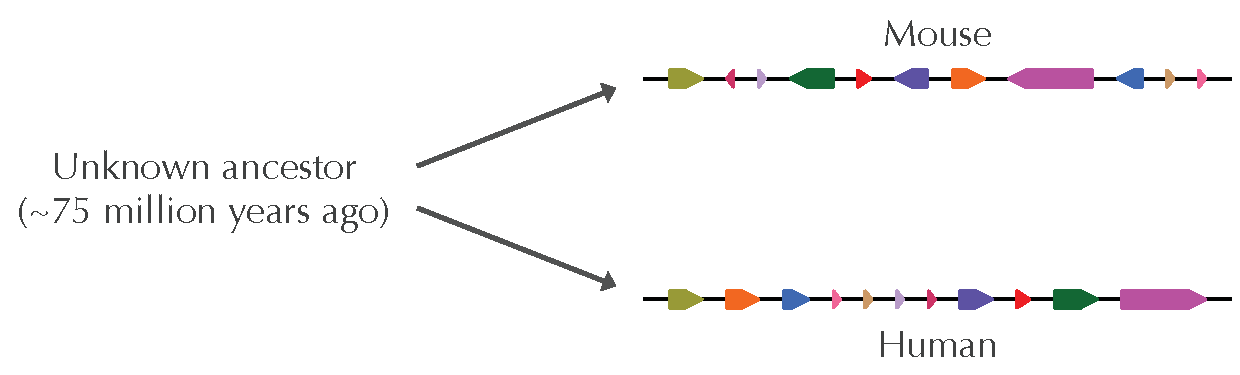
\includegraphics[width=0.88\textwidth]{images/rearrangements/mouse_and_human_synteny_blocks}
\caption{Mouse and human X chromosomes represented as 11 colored, directed segments (synteny blocks).}
\label{fig:mouse_and_human_synteny_blocks}
\end{figure}

\autoref{fig:mouse_and_human_synteny_blocks} offers a compact representation of how the human and mouse X chromosomes differ, but what does it really mean?  It turns out not only that most human genes have mouse counterparts, but also that hundreds of similar genes often line up one after another in the same order in the two species genomes. Each of the 11 colored segments in \autoref{fig:mouse_and_human_synteny_blocks} represents such a procession of similar genes and is called a \textdef{synteny block}. Later, we will explain how to construct synteny blocks and what the left and right \textdef{directions} of the blocks signify.

Synteny blocks simplify the comparison of the mouse and human X chromosomes from 150 million base pairs to only 11 units. This simplification is analogous to comparing two similar photographs. If we compare the images one pixel at a time, we may be overwhelmed by the scale of the problem; instead, we need to zoom out in order to notice higher-level patterns.  It is no accident that biologists use the term ``resolution'' to discuss the level at which genomes are analyzed.

\phantomsection
\subsection{Reversals}
\label{subsec:reversals}

You have probably been wondering how the genome changes when it undergoes a genome rearrangement. Genome rearrangements were discovered 90 years ago when Alfred Sturtevant was studying fruit fly mutants with scarlet- and peach-colored eyes as well as abnormally shaped deltoid wings. Sturtevant determined the genes coding for these traits, called \Red{scarlet}, \Orange{peach}, and \Blue{delta}, and he was amazed to find that the arrangement of these genes in \textit{Drosophila melanogaster} (\Red{scarlet}, \Orange{peach}, \Blue{delta}) differed from their arrangement in \textit{Drosophila simulans} (\Red{scarlet}, \Blue{delta}, \Orange{peach}). He immediately conjectured that the chromosomal segment containing \Orange{peach} and \Blue{delta} must have been flipped around (see \takedetour[Discovery of Genome Rearrangements]{discovery_of_genome_rearrangements}). Sturtevant had witnessed the most common form of genome rearrangement, called a \textdef{reversal}, which flips around an interval of a chromosome and inverts the directions of any synteny blocks within the interval.

\autoref{fig:transforming_mouse_into_human_7_reversals} shows a series of 7 reversals transforming the mouse X chromosome into the human X chromosome.  If this scenario is correct, then the X chromosome of the ancestor of humans and mice must be represented by one of the intermediate synteny block orderings.  Unfortunately, this series of 7 reversals offers only one of 1070 different 7-step scenarios transforming the mouse X chromosome into the human X chromosome. We have no clue which scenario is correct, or even whether the correct scenario had exactly 7 reversals.\\

\begin{qbox}[
Can you convert the mouse X chromosome into the human X chromosome using only 6 reversals?
]\end{qbox}

\begin{figure}[h]
\mySfFamily
\centering
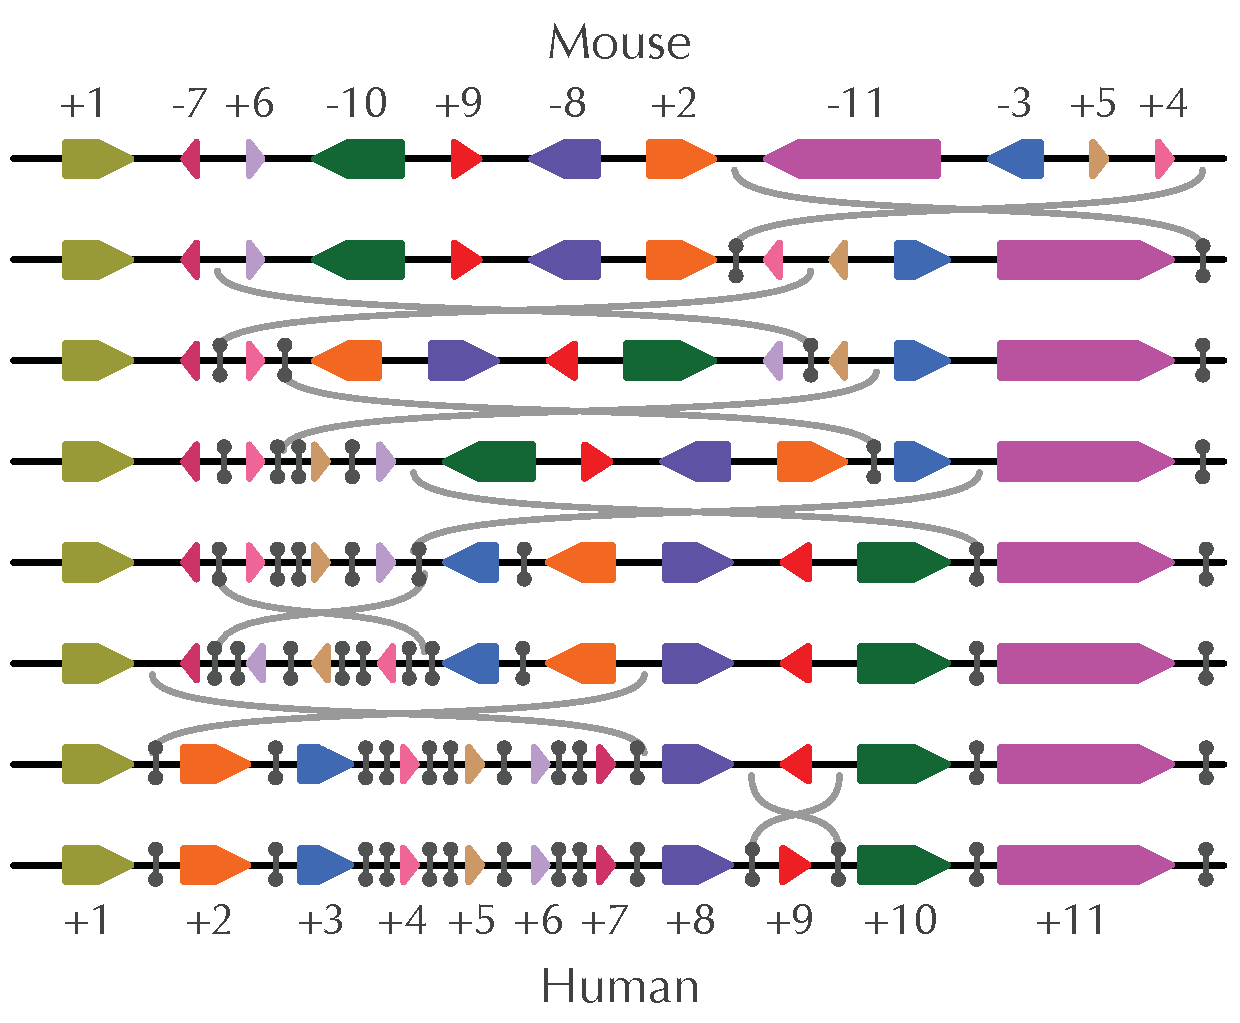
\includegraphics[width=0.8\textwidth]{images/rearrangements/transforming_mouse_into_human_7_reversals}
\caption{Transforming the mouse X chromosome into the human X chromosome with 7 reversals. Each synteny block is uniquely colored and labeled with an integer between 1 and 11; the positive or negative sign of each integer indicates the synteny block's direction (pointing right or left, respectively). Two short vertical segments delineate the endpoints of the inverted interval in each reversal. Suppose that this evolutionary scenario is correct and that, say, the 5th synteny block arrangement from the top presents the true ancestral arrangement. Then the first 4 reversals happened on the evolutionary path from mice to the human-mouse common ancestor (traveling backward in time), and the final 3 reversals happened on the evolutionary path from the common ancestor
to humans (traveling forward in time).  In this chapter, we are not interested in reconstructing the ancestral genome and thus are not concerned with whether a certain reversal travels backward or forward in time.}
\label{fig:transforming_mouse_into_human_7_reversals}
\end{figure}

\noindent Regardless of how many reversals separate the human and mouse X chromosomes, you can see that reversals must be rare genomic events.  Indeed, genome rearrangements typically cause the death or sterility of the mutated organism, thus preventing it from passing the rearrangement on to the next generation.  However, a tiny fraction of genome rearrangements may have a positive effect on survival and propagate through a species as the result of natural selection.  When a population becomes isolated from the rest of its species for long enough, the work of rearrangements can even create a new species.

\phantomsection
\subsection{Rearrangement hotspots}
\label{subsec:rearrangement_hotspots}

Geology provides a thought-provoking analogy for thinking about genome evolution.  You might like to think of genome rearrangements as ``genomic earthquakes'' that dramatically change the chromosomal architecture of an organism.  Genome rearrangements contrast with much more frequent point mutations, which work slowly and are analogous to ``genomic erosion''.

You can visualize a reversal as breaking the genome on both sides of a chromosomal interval, flipping the interval, and then gluing the resulting segments in a new order. Keeping in mind that earthquakes occur more frequently in specific locations on Earth, we wonder if a similar principle holds for reversals --- are they happening over and over again in specific genomic regions?  A fundamental question in chromosome evolution studies is whether the \textdef{breakpoints} of reversals (i.e., the the ends of the inverted intervals) occur along ``fault lines'' called \textdef{rearrangement hotspots}. If such hotspots exist in the human genome, we want to locate them and determine how they might relate to genetic disorders, which are often attributable to rearrangements.

Of course, we should rigorously define what we mean by a ``rearrangement hotspot''. Re-examining the 7-reversal scenario changing the mouse X chromosome into the human X chromosome in \autoref{fig:transforming_mouse_into_human_7_reversals}, we record the endpoints of each reversal using vertical segments. Regions affected by multiple reversals are indicated by multiple vertical segments in the human X chromosome. For example, the region adjacent to the pointed side of block 3 in \autoref{fig:transforming_mouse_into_human_7_reversals} is used as an endpoint of both the 4th and 5th reversals. As a result, we have placed two vertical lines between blocks 3 and 4 in the human X chromosome. However, just because we showed two breakpoints in this region does not imply that this region is a rearrangement hotspot, since the reversals in \autoref{fig:transforming_mouse_into_human_7_reversals} represent just one possible evolutionary scenario. Because the true rearrangement scenario is unknown, it is not immediately clear how we could determine whether rearrangement hotspots exist.\\

\phantomsection
\FloatBarrier
\section{The Random Breakage Model of Chromosome Evolution}
\label{sec:the_random_breakage_model_of_chromosome_evolution}

In 1973, Susumu Ohno proposed the \textdef{Random Breakage Model} of chromosome evolution.  This hypothesis states that the breakpoints of rearrangements are selected randomly, implying that rearrangement hotspots in mammalian genomes do not exist.  Yet this model lacked supporting evidence when it was introduced.  After all, how could we possibly determine whether rearrangement hotspots exist without knowing the exact sequence of rearrangements separating two species?\\

\begin{qbox}[
Consider the following questions.
\vspace{-1ex}
\begin{enumerate}
\item Say that a series of random reversals result in one huge synteny block covering 90\% of the genome in addition to 99 tiny synteny blocks covering the remaining 10\% of the genome.  Should we be surprised?
\vspace{-1ex}
\item What if random reversals result in 100 synteny blocks of roughly the same length? Should we be surprised?
\end{enumerate}
\vspace{-1ex}
]\end{qbox}

\noindent The idea that we wish to impress on you in the preceding questions is that we can test the Random Breakage Model by analyzing the distribution of synteny block lengths. For example, the lengths of the human-mouse synteny blocks on the X chromosome vary widely, with the largest block (block 11 in \autoref{fig:transforming_mouse_into_human_7_reversals}) taking up nearly 25\% of the entire length of the X chromosome. Is this variation in synteny block length consistent with the Random Breakage Model?\\

\begin{figure}[h]
\centering
\begin{tabular}{c}
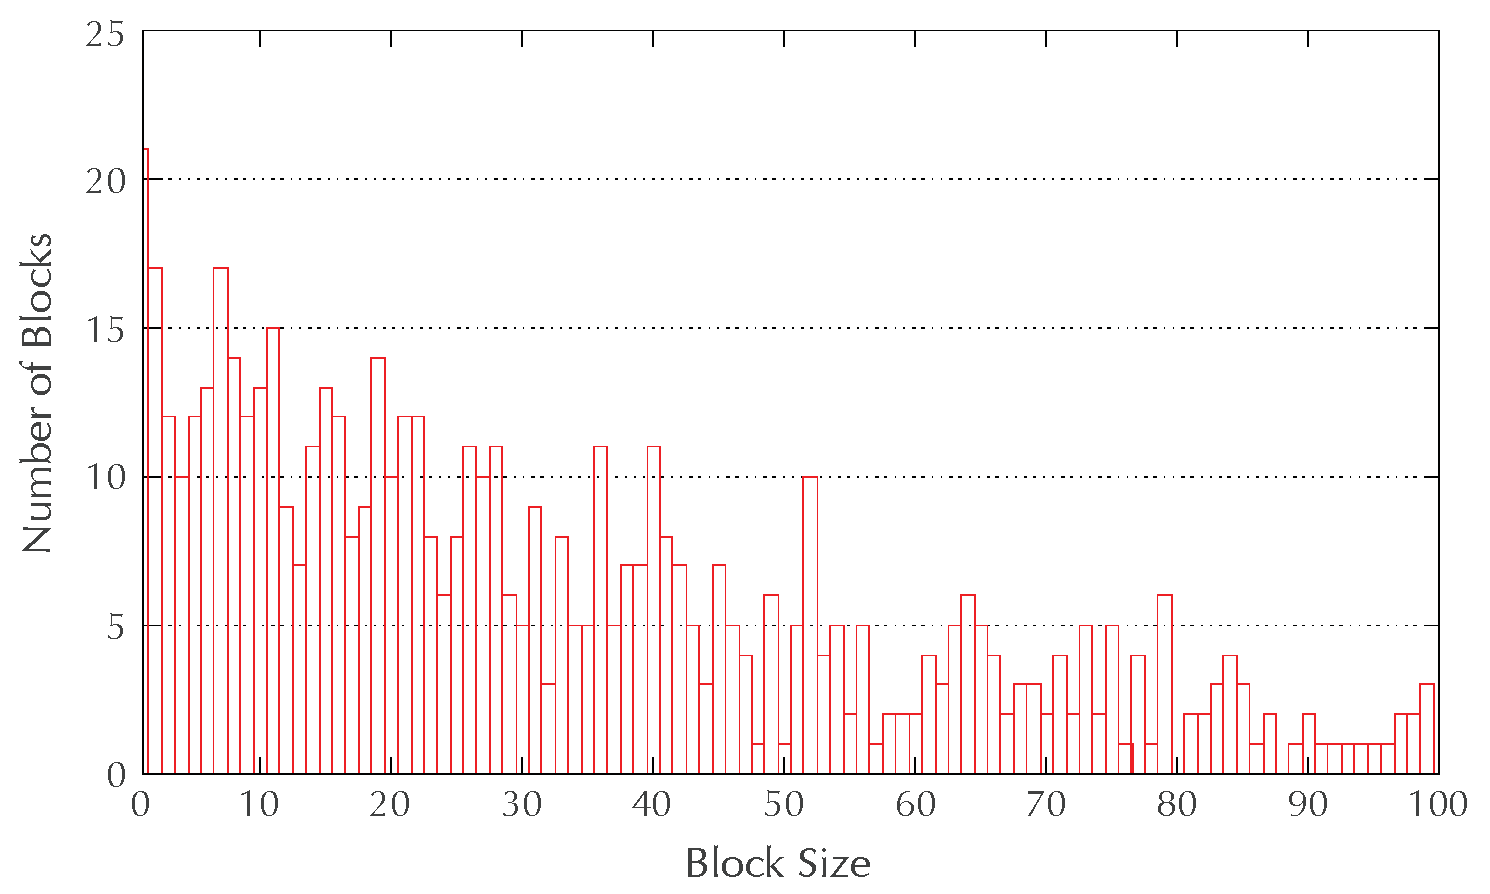
\includegraphics[width = 0.65\textwidth]{images/rearrangements/histogram_exponential_distribution_one_run}\\[2ex]
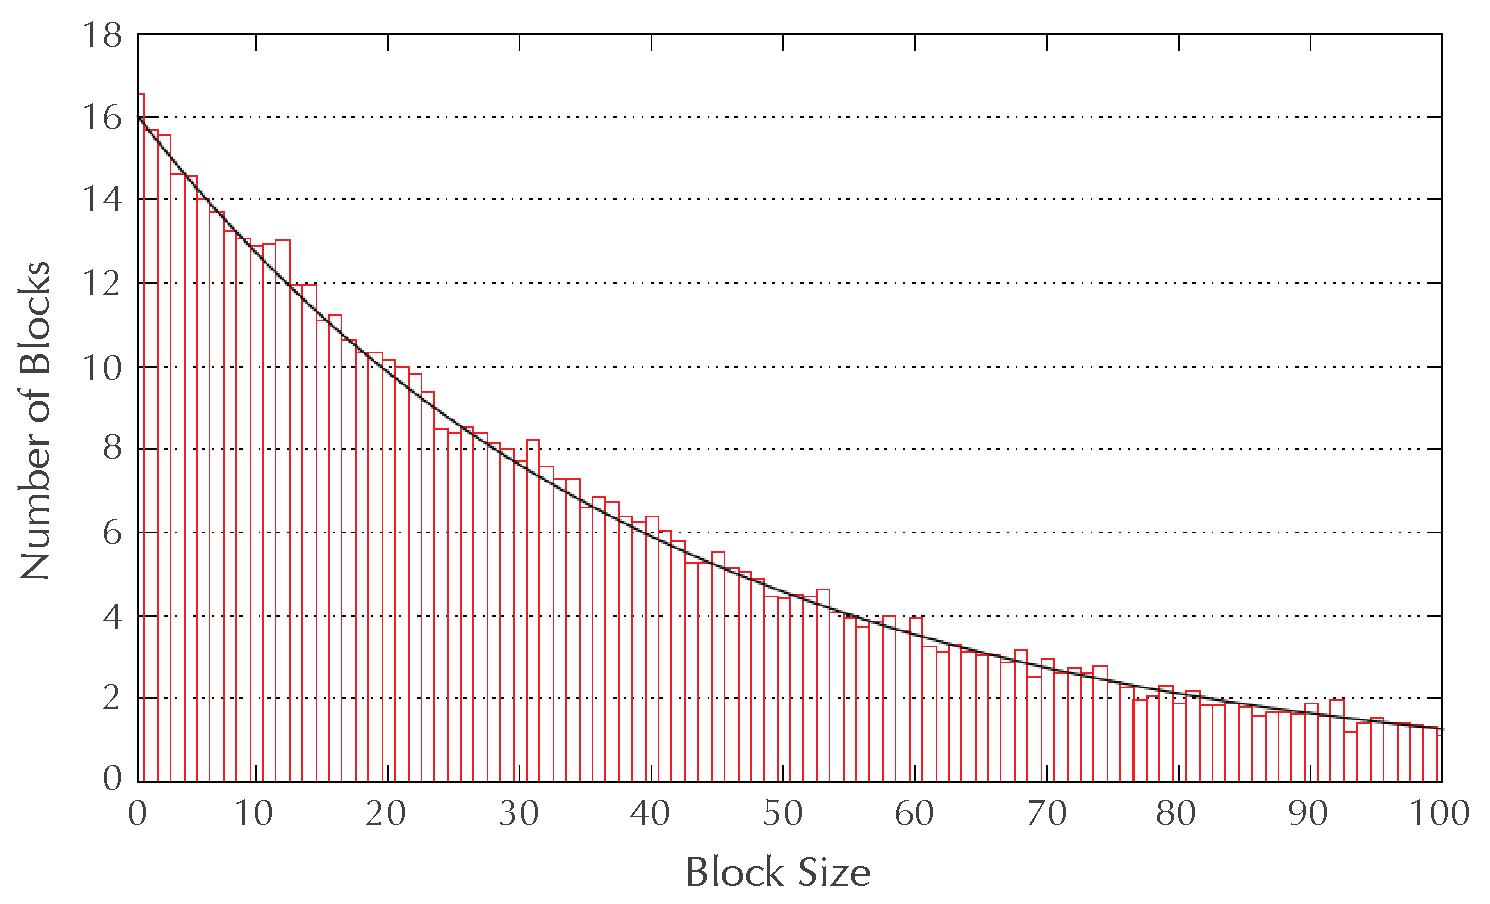
\includegraphics[width = 0.65\textwidth]{images/rearrangements/histogram_exponential_distribution_many_runs}
\end{tabular}
\caption{(Top) A histogram showing the number of blocks of each size (for a simulated genome with 25,000 genes after 320 randomly chosen reversals). Blocks having more than 100 genes are not shown. (Bottom) An average histogram of synteny block lengths for 100 simulations, fitted by the exponential distribution.}
\label{fig:histogram_exponential_distribution}
\end{figure}

In 1984, Joseph Nadeau and Benjamin Taylor asked what the expected lengths of synteny blocks should be after $N$ reversals occurring at random locations in the genome.  If we rule out the unlikely event that two random reversals cut the chromosome in exactly the same position, then $N$ random reversals cut the chromosome in $2N$ locations and produce $2N + 1$ synteny blocks. \autoref{fig:histogram_exponential_distribution} (top) depicts the result of a computational experiment in which 320 random reversals are applied to a simulated chromosome consisting of 25,000 genes, producing $2 \cdot 320+1 = 641$ synteny blocks. The average synteny block size is 25,000$/641 \approx 34$ genes, but this does not mean that all synteny blocks should have approximately 34 genes. If we select random locations for breakpoints, then some blocks may have only a few genes, whereas other blocks may contain over a hundred.  The point is that regardless of how many times we run this simulation, the resulting distributions of synteny block lengths will be similar. \autoref{fig:histogram_exponential_distribution} (bottom) averages the results of 100 such simulations and illustrates that the distribution of synteny block lengths can be approximated by a curve corresponding to an \textdef{exponential distribution} (see \takedetour[The Exponential Distribution]{the_exponential_distribution}).  The exponential distribution predicts that we should observe about seven blocks having 34 genes and one or two much larger blocks having 100 genes.

What happens when we look at the histogram for the real human and mouse synteny blocks? When Nadeau and Taylor constructed this histogram for the limited genetic data available in 1984, they observed that the lengths of blocks fit the exponential distribution well.  In the 1990s, more accurate synteny block data fit the exponential distribution even better (\autoref{fig:histogram_human_mouse_synteny_blocks}). Case closed --- even though we don't know the exact rearrangements causing our genome to evolve over the last 75 million years, these rearrangements must have followed the Random Breakage Model!\\

\begin{figure}[h]
\mySfFamily
\centering
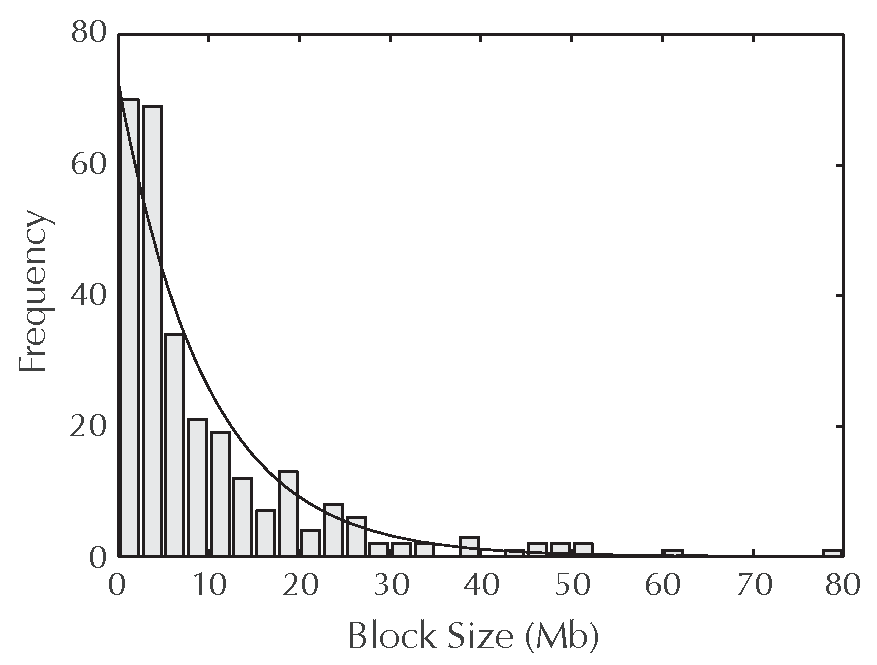
\includegraphics[width=0.45\textwidth]{images/rearrangements/histogram_human_mouse_synteny_blocks}
\caption{Histogram of human-mouse synteny block lengths (only synteny blocks longer than 1 million nucleotides are shown). The histogram is fitted by an exponential distribution.}
\label{fig:histogram_human_mouse_synteny_blocks}
\end{figure}

\begin{qbox}[
Do you agree with the logic behind this argument?
]\end{qbox}

\vspace{-2\baselineskip}

\phantomsection
\FloatBarrier
\section{Sorting by Reversals}
\label{sec:sorting_by_reversals}

We now have evidence in favor of the Random Breakage Model, but this evidence is far from conclusive.  To test this model, let's start building a mathematical model for rearrangement analysis.  We will therefore return to a problem that we hinted at the introduction, which is finding the minimum number of reversals that could transform the mouse X chromosome into the human X chromosome.\\

\begin{qbox}[
From a biological perspective, why do you think we want to find the minimum possible number of reversals?
]\end{qbox}

\noindent We ask for the minimum number of reversals in accordance with the principle of \textdef{Occam's razor}. This maxim states that when presented with some quandary, we should explain it using the simplest hypothesis that is consistent with what we already know. In this case, it seems most reasonable that evolution would take the ``shortest path'' connecting two species, i.e., the most \textdef{parsimonious} evolutionary scenario. Evolution may not always take the shortest path, but even when it does not, the number of steps in the true evolutionary scenario often comes close to the number of steps in the most parsimonious scenario.  How, then, can we find the length of this shortest path?

Genome rearrangement studies typically ignore the lengths of synteny blocks and represent chromosomes by \textdef{signed permutations}. Each block is labeled by a number, which is assigned a positive/negative sign depending on the block's direction.  The number of elements in a signed permutation is its \textdef{length}. As you can see from \autoref{fig:transforming_mouse_into_human_7_reversals}, the human and mouse X chromosomes can be represented by the following signed permutations of length 11:

\begin{center}
\tabcolsep = 0.3em
\begin{tabular}{rr @{\hskip 0em} rrrrrrrrrrrl}
\textbf{Mouse:} & ( & $+1$ & $-7$ & $+6$ & $-10$ & $+9$ & $-8$ & $+2$ & $-11$ & $-3$ & $+5$ & $+4)$\\
\textbf{Human:} & ( & $+1$ & $+2$ & $+3$ & $+4$ & $+5$ & $+6$ & $+7$ & $+8$ & $+9$ & $+10$ & $+11)$
\end{tabular}
\end{center}

\noindent In the rest of the chapter, we will refer to signed permutations as \textdef{permutations} for short. Because we assume that each synteny block is unique, we do not allow repeated numbers in permutations (e.g., $(+1$ $-2$ $+3$ $+2)$ is not a permutation).\\

\begin{exercise}[
How many permutations of length $n$ are there?
]\end{exercise}

\vspace{-0.5\baselineskip}

\noindent We can model reversals by inverting the elements within an interval of a permutation, then switching the signs of any elements within the inverted interval. For example, the cartoon in \autoref{fig:reversal_cartoon} illustrates how a reversal changes the permutation $(+1$ $+2$ $+3$ $\MathRed{+4}$ $\MathRed{+5}$ $\MathRed{+6}$ $\MathRed{+7}$ $\MathRed{+8}$ $+9$ $+10)$ into $(+1$ $+2$ $+3$ $\MathRed{-8}$ $\MathRed{-7}$ $\MathRed{-6}$ $\MathRed{-5}$ $\MathRed{-4}$ $+9$ $+10)$.  This reversal can be viewed as first breaking the permutation between +3 and +4 as well as between +8 and +9:

\begin{center}
$(+1$ $+2$ $+3)$$(\MathRed{+4}$ $\MathRed{+5}$ $\MathRed{+6}$ $\MathRed{+7}$ $\MathRed{+8})$$(+9$ $+10)$
\end{center}

\begin{figure}[t]
\centering
\begin{tabular}{c @{\hskip 2.5em} c}
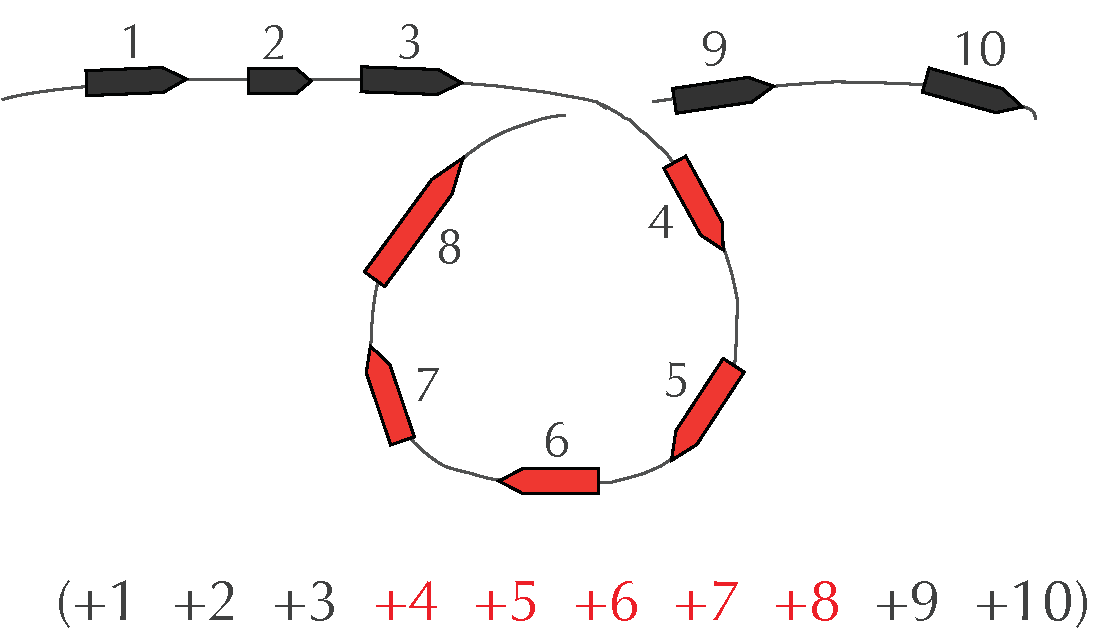
\includegraphics[width = 0.4\textwidth]{images/rearrangements/reversal_cartoon-1} & 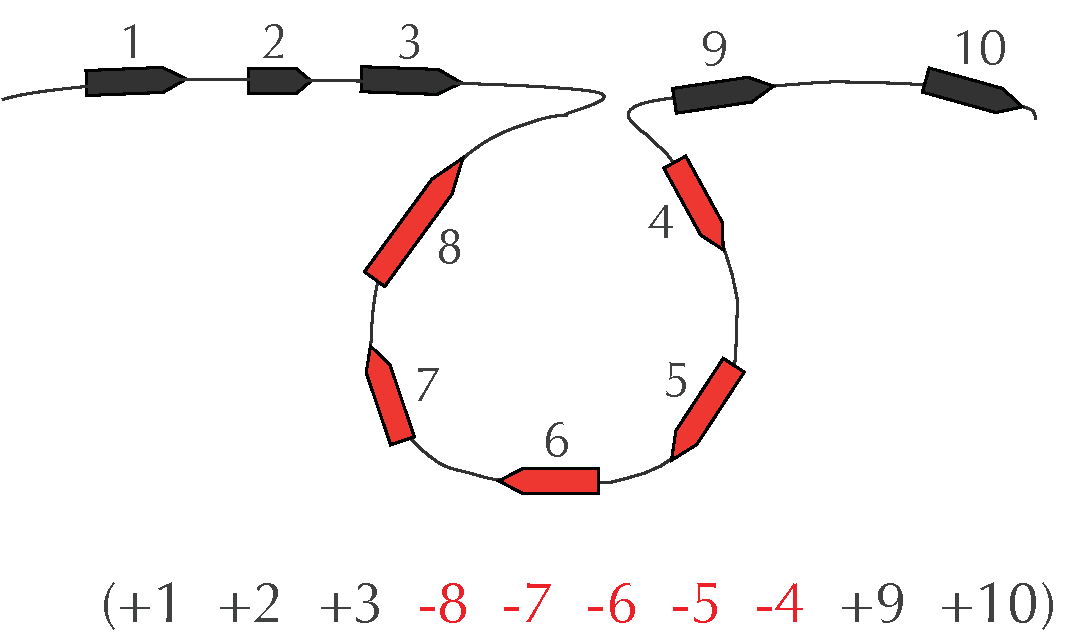
\includegraphics[width = 0.4\textwidth]{images/rearrangements/reversal_cartoon-2}
\end{tabular}
\caption{A cartoon illustrating how a reversal breaks a chromosome in two places and inverts the segment between the two breakpoints. Note that the reversal changes the sign of each element within the permutation's inverted segment.}
\label{fig:reversal_cartoon}
\end{figure}

\noindent It then inverts this middle segment:

\begin{center}
$(+1$ $+2$ $+3)$$(\MathRed{-8}$ $\MathRed{-7}$ $\MathRed{-6}$ $\MathRed{-5}$ $\MathRed{-4})$$(+9$ $+10)$
\end{center}

\noindent and finally glues the three segments back together to form a new permutation:

\begin{center}
$(+1$ $+2$ $+3$ $\MathRed{-8}$ $\MathRed{-7}$ $\MathRed{-6}$ $\MathRed{-5}$ $\MathRed{-4}$ $+9$ $+10)$
\end{center}

\fudgespace

\begin{exercise}[
How many different reversals can be applied to a permutation of length $n$?
]\end{exercise}

\noindent We define the \textdef{reversal distance} between permutations $P$ and $Q$, denoted $d_{\text{rev}}(P, Q)$, as the minimum number of reversals required to transform $P$ into $Q$.\\

\begin{problem}[Reversal Distance Problem]{Calculate the reversal distance between two permutations.}{Two permutations of equal length.}{The reversal distance between these permutations.}
\end{problem}

\vspace{-\baselineskip}

\noindent We represented the human X chromosome by $(+1$ $+2$ $+3$ $+4$ $+5$ $+6$ $+7$ $+8$ $+9$ $+10$ $+11)$; this permutation, in which blocks are ordered from smallest to largest with positive directions, is called the \textdef{identity permutation}. The reason why we used the identity permutation of length 11 to represent the human X chromosome is that when comparing two genomes, we can label the synteny blocks in one of the genomes however we like. The block labeling for which the human X chromosome is the identity permutation automatically induces the representation of the mouse chromosome as $(+1$ $-7$ $+6$ $-10$ $+9$ $-8$ $+2$ $-11$ $-3$ $+5$ $+4)$.   Of course, we could have instead encoded the mouse X chromosome as the identity permutation, which would have induced the encoding of the human X chromosome as $(+1$ $+7$ $-9$ $+11$ $+10$ $+3$ $-2$ $-6$ $+5$ $-4$ $-8)$ (\autoref{fig:x_chromosomes_different_encoding}).\\

\begin{figure}[h]
\centering
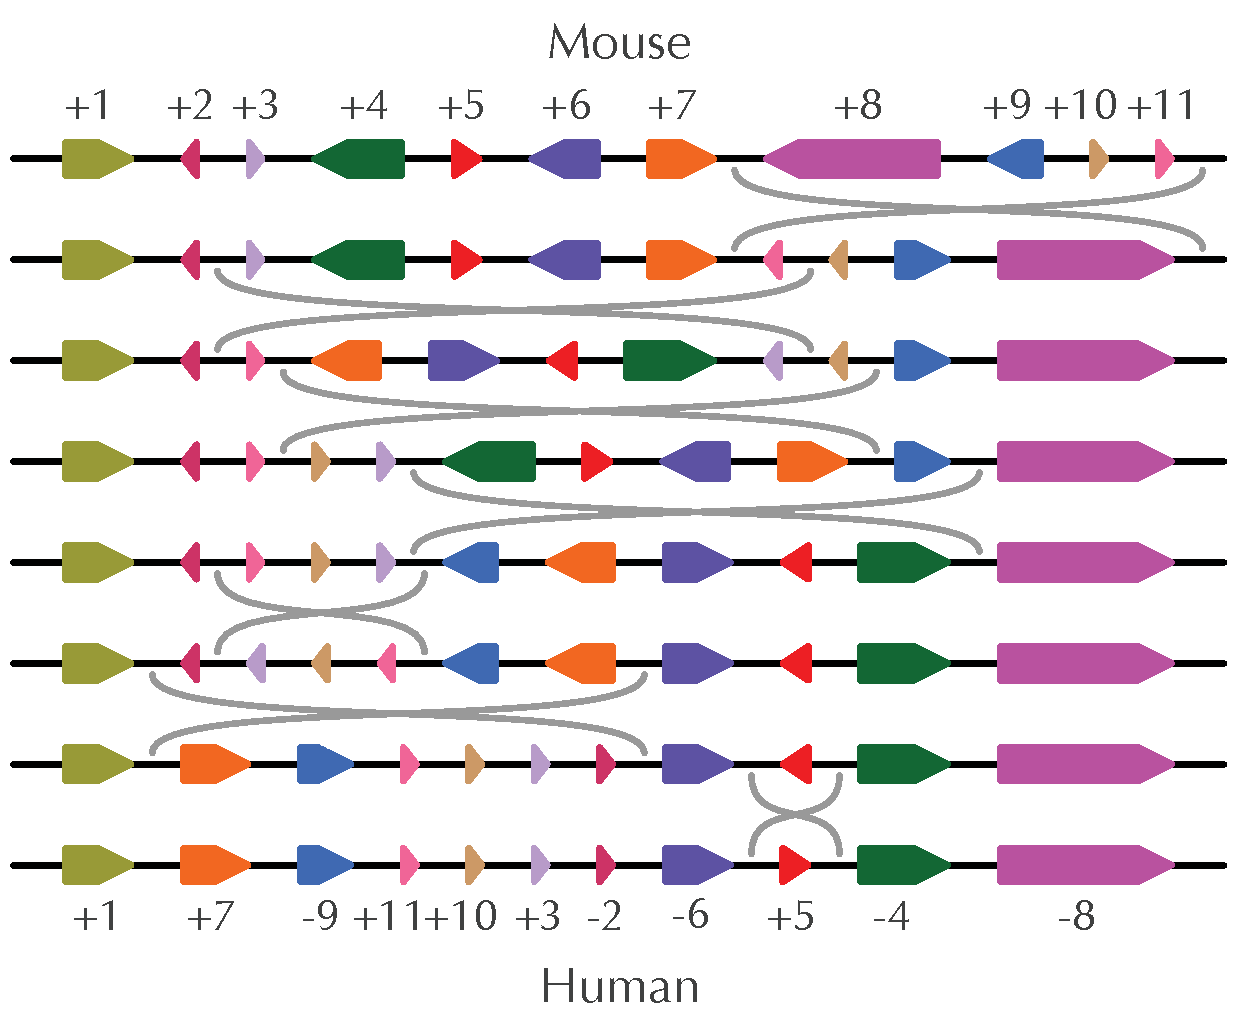
\includegraphics[width = 0.8\textwidth]{images/rearrangements/x_chromosomes_different_encoding}
\caption{Encoding the mouse X chromosome as the identity permutation implies encoding the human X chromosome as $(+1$ $+7$ $-9$ $+11$ $+10$ $+3$ $-2$ $-6$ $+5$ $-4$ $-8)$.}
\label{fig:x_chromosomes_different_encoding}
\end{figure}

\begin{qbox}[
Is the reversal distance between $(+1$ $+2$ $+3$ $+4$ $+5$ $+6$ $+7$ $+8$ $+9$ $+10$ $+11)$ and $(+1$ $-7$ $+6$ $-10$ $+9$ $-8$ $+2$ $-11$ $-3$ $+5$ $+4)$ equal to the reversal distance between $(+1$ $+2$ $+3$ $+4$ $+5$ $+6$ $+7$ $+8$ $+9$ $+10$ $+11)$ and $(+1$ $+7$ $-9$ $+11$ $+10$ $+3$ $-2$ $-6$ $+5$ $-4$ $-8)$?  In other words, does the specific labeling of synteny blocks affect the reversal distance between the two chromosomes?
]\end{qbox}

\noindent Because we have the freedom to label synteny blocks however we like, we will consider an offshoot of the Reversal Distance Problem in which permutation $Q$ is the identity permutation  $(+1$ $+2$ \ldots $+n)$. This computational problem is called \textdef{sorting by reversals}, and we denote the minimum number of reversals required to sort $P$ into the identity permutation as $d_{\text{rev}}(P)$.  The history of sorting by reversals is founded in a culinary application and involves two celebrities (see \takedetour[Bill Gates and David X. Cohen Flip Pancakes]{bill_gates_and_david_x_cohen_flip_pancakes}).\\

\begin{problem}[Sorting by Reversals Problem]{Compute the reversal distance between a permutation and the identity permutation.}{A permutation $P$.}{The reversal distance $d_{\text{rev}}(P)$.}
\end{problem}

\noindent Here is a sorting of $(+2$ $-4$ $-3$ $+5$ $-8$ $-7$ $-6$ $+1)$ using five reversals, with the inverted interval at each step shown in red:

\begin{center}
\begin{math}
\arraycolsep = 0.3em
\begin{array}{r @{\hskip 0em} r r r r r r r r @{\hskip 0em} l}
( & +2 & \MathRed{-4} & \MathRed{-3} & +5 & -8 & -7 & -6 & +1 &)\\[-0.25ex]
( & +2 & +3 & +4 & +5 & \MathRed{-8} & \MathRed{-7} & \MathRed{-6} & +1 &)\\[-0.25ex]
( & +2 & +3 & +4 & +5 & +6 & +7 & +8 & \MathRed{+1} &)\\[-0.25ex]
( & \MathRed{+2} & \MathRed{+3} & \MathRed{+4} & \MathRed{+5} & \MathRed{+6} & \MathRed{+7} & \MathRed{+8} & -1 &)\\[-0.25ex]
( & \MathRed{-8} & \MathRed{-7} & \MathRed{-6} & \MathRed{-5} & \MathRed{-4} & \MathRed{-3} & \MathRed{-2} & \MathRed{-1} &)\\[-0.25ex]
( & +1 & +2 & +3 & +4 & +5 & +6 & +7 & +8 &)
\end{array}
\end{math}
\end{center}

\begin{qbox}[
Can you sort this permutation using fewer reversals?
]\end{qbox}

\vspace{-0.5\baselineskip}

\noindent Here is a faster sorting:

\begin{center}
\begin{math}
\arraycolsep = 0.3em
\begin{array}{r @{\hskip 0em} r r r r r r r r @{\hskip 0em} l}
( & +2 & \MathRed{-4} & \MathRed{-3} & +5 & -8 & -7 & -6 & +1 &)\\[-0.25ex]
( & \MathRed{+2} & \MathRed{+3} & \MathRed{+4} & \MathRed{+5} & -8 & -7 & -6 & +1 &)\\[-0.25ex]
( & -5 & -4 & -3 & -2 & \MathRed{-8} & \MathRed{-7} & \MathRed{-6} & \MathRed{+1} &)\\[-0.25ex]
( & \MathRed{-5} & \MathRed{-4} & \MathRed{-3} & \MathRed{-2} & \MathRed{-1} & +6 & +7 & +8 &)\\[-0.25ex]
( & +1 & +2 & +3 & +4 & +5 & +6 & +7 & +8 &)
\end{array}
\end{math}
\end{center}

\begin{qbox}[
Consider the following questions.
\vspace{-1ex}
\begin{enumerate}
\item Is it possible to sort this permutation even faster?
\vspace{-1ex}
\item During sorting by reversals, the intermediate permutations in the example above are getting more and more ``ordered''. Can you come up with a quantitative measure of how ordered a permutation is?
\vspace{-1ex}
\end{enumerate}
]\end{qbox}

%\vspace{-2\baselineskip}

\phantomsection
\FloatBarrier
\section{A Greedy Algorithm for Sorting by Reversals}
\label{sec:a_greedy_algorithm_for_sorting_by_reversals}

Let's see if we can design a greedy heuristic to approximate $d_{\text{rev}}(P)$. The simplest idea is to first fix $+1$ in the first position, then fix $+2$ in the second position, and so on.  For example, element 1 is already in the correct position and has the correct sign in the mouse X chromosome, but element 2 is not in the correct position. We can keep element 1 fixed and move element 2 to the correct position by applying a single reversal.

\begin{center}
\begin{math}
\arraycolsep = 0.3em
\begin{array}{r @{\hskip 0em} r r r r r r r r r r r @{\hskip 0em} l}
( & \MathBlue{+1} & \MathRed{-7} & \MathRed{+6} & \MathRed{-10} & \MathRed{+9} & \MathRed{-8} & \MathRed{+2} & -11 & -3 & +5 & +4 &)\\[-0.25ex]
( & \MathBlue{+1} & -2 & +8 & -9 & +10 & -6 & +7 & -11 & -3 & +5 & +4 &)\\
\end{array}
\end{math}
\end{center}

\noindent One more reversal flips element 2 around so that it has the correct sign:

\begin{center}
\begin{math}
\centering
\arraycolsep = 0.3em
\begin{array}{r @{\hskip 0em} r r r r r r r r r r r  @{\hskip 0em} l}
( & \MathBlue{+1} & \MathRed{-2} & +8 & -9 & +10 & -6 & +7 & -11 & -3 & +5 & +4 &)\\[-0.25ex]
( & \MathBlue{+1} & \MathBlue{+2} & +8 & -9 & +10 & -6 & +7 & -11 & -3 & +5 & +4 &)
\end{array}
\end{math}
\end{center}

\noindent By iterating, we can successively move larger and larger elements to their correct positions in the identity permutation by following the reversals below.  The inverted interval of each reversal is still shown in red, and elements that have been placed in the correct position are shown in blue.

\begin{center}
\begin{math}
\arraycolsep = 0.2em
\begin{array}{r @{\hskip 0em} r r r r r r r r r r r @{\hskip 0em} l}
( & \MathBlue{+1} & \MathRed{-7} & \MathRed{+6} & \MathRed{-10} & \MathRed{+9} & \MathRed{-8} & \MathRed{+2} & -11 & -3 & +5 & +4 &)\\[-0.25ex]
( & \MathBlue{+1} & \MathRed{-2} & +8 & -9 & +10 & -6 & +7 & -11 & -3 & +5 & +4 &)\\[-0.25ex]
( & \MathBlue{+1} & \MathBlue{+2} & \MathRed{+8} & \MathRed{-9} & \MathRed{+10} & \MathRed{-6} & \MathRed{+7} & \MathRed{-11} & \MathRed{-3} & +5 & +4 &)\\[-0.25ex]
( & \MathBlue{+1} & \MathBlue{+2} & \MathBlue{+3} & \MathRed{+11} & \MathRed{-7} & \MathRed{+6} & \MathRed{-10} & \MathRed{+9} & \MathRed{-8} & \MathRed{+5} & \MathRed{+4} &)\\[-0.25ex]
( & \MathBlue{+1} & \MathBlue{+2} & \MathBlue{+3} & \MathRed{-4} & -5 & +8 & -9 & +10 & -6 & +7 & -11 &)\\[-0.25ex]
( & \MathBlue{+1} & \MathBlue{+2} & \MathBlue{+3} & \MathBlue{+4} & \MathRed{-5} & +8 & -9 & +10 & -6 & +7 & -11 &)\\[-0.25ex]
( & \MathBlue{+1} & \MathBlue{+2} & \MathBlue{+3} & \MathBlue{+4} & \MathBlue{+5} & \MathRed{+8} & \MathRed{-9} & \MathRed{+10} & \MathRed{-6} & +7 & -11 &)\\[-0.25ex]
( & \MathBlue{+1} & \MathBlue{+2} & \MathBlue{+3} & \MathBlue{+4} & \MathBlue{+5} & \MathBlue{+6} & \MathRed{-10} & \MathRed{+9} & \MathRed{-8} & \MathRed{+7} & -11 &)\\[-0.25ex]
( & \MathBlue{+1} & \MathBlue{+2} & \MathBlue{+3} & \MathBlue{+4} & \MathBlue{+5} & \MathBlue{+6} & \MathRed{-7} & +8 & -9 & +10 & -11 &)\\[-0.25ex]
( & \MathBlue{+1} & \MathBlue{+2} & \MathBlue{+3} & \MathBlue{+4} & \MathBlue{+5} & \MathBlue{+6} & \MathBlue{+7} & \MathBlue{+8} & \MathRed{-9} & +10 & -11 &)\\[-0.25ex]
( & \MathBlue{+1} & \MathBlue{+2} & \MathBlue{+3} & \MathBlue{+4} & \MathBlue{+5} & \MathBlue{+6} & \MathBlue{+7} & \MathBlue{+8} & \MathBlue{+9} & \MathBlue{+10} & \MathRed{-11} &)\\[-0.25ex]
( & \MathBlue{+1} & \MathBlue{+2} & \MathBlue{+3} & \MathBlue{+4} & \MathBlue{+5} & \MathBlue{+6} & \MathBlue{+7} & \MathBlue{+8} & \MathBlue{+9} & \MathBlue{+10} & \MathBlue{+11} &)\\[-0.25ex]
\end{array}
\end{math}
\end{center}

This example motivates a greedy heuristic called \textalg{GreedySorting}.  We say that element $k$ in permutation $P = (p_1 \ldots p_n)$ is \textdef{sorted} if $p_k = +k$ and \textdef{unsorted} otherwise.  For every unsorted element $k$ that is located outside the first $k$ positions in $P$, there exists a single reversal, called the \textdef{\textit{k}-sorting reversal}, which fixes the first $k - 1$ elements of $P$ and moves element $k$ to the $k$-th position.  For example, in the sorting of the mouse X chromosome shown above, the 2-sorting reversal transforms $(\MathBlue{+1}$ $\MathRed{-7}$ $\MathRed{+6}$ $\MathRed{-10}$ $\MathRed{+9}$ $\MathRed{-8}$ $\MathRed{+2}$ $-11$ $-3$ $+5$ $+4)$ into $(\MathBlue{+1}$ $-2$ $+8$ $-9$ $+10$ $-6$ $+7$ $-11$ $-3$ $+5$ $+4)$.  In this case, one additional reversal flipping $-2$ around was needed to sort element 2.

We now give the pseudocode for \textalg{GreedySorting}, which applies $k$-sorting reversals for increasing values of $k$.  Here, $|P|$ refers to the length of permutation $P$.\\

\begin{elaboration}
\begin{algorithmic}
\leftskip = \algindent %Needed to match the indentation of the text.
\Algorithm{GreedySorting}{\textvar{P}}
	\State $\textvar{approxReversalDistance} \gets 0$
	\For {$k \gets 1$ to $|P|$}
		\If {element $k$ is not sorted}
			\State apply the $k$-sorting reversal to $P$
			\State $\textvar{approxReversalDistance} \gets \textvar{approxReversalDistance} + 1$
			\If {$k$-th element of $P$ is $-k$}
				\State apply the reversal flipping the $k$-th element of $P$
				\State $\textvar{approxReversalDistance} \gets \textvar{approxReversalDistance} + 1$
			\EndIf
		\EndIf
	\EndFor
	\State \return{~\textvar{approxReversalDistance}}
\EndAlgorithm
\end{algorithmic}
\end{elaboration}
\protect\computationalproblem[Implement \textalg{GreedySorting}]{-21.68}

\noindent In the case of the mouse X chromosome, \textalg{GreedySorting} requires 11 reversals, but we already know that this permutation can be sorted with 7 reversals, which causes us to wonder: how good of a heuristic is \textalg{GreedySorting}?\\

\begin{exercise}[
What is the largest number of reversals \textalg{GreedySorting} could ever require to sort a permutation of length $n$?
]\end{exercise}

\noindent Consider the permutation $(-6$ $+1$ $+2$ $+3$ $+4$ $+5)$.  You can verify that the greedy heuristic requires ten steps to sort this permutation, and yet it can be sorted using just two reversals!

\begin{center}
\begin{math}
\arraycolsep = 0.3em
\begin{array}{r @{\hskip 0em} r r r r r r @{\hskip 0em} l}
( & \MathRed{-6} & \MathRed{+1} & \MathRed{+2} & \MathRed{+3} & \MathRed{+4} & \MathRed{+5} &)\\[-0.25ex]
( & \MathRed{-5} & \MathRed{-4} & \MathRed{-3} & \MathRed{-2} & \MathRed{-1} & +6 &)\\[-0.25ex]
( & +1 & +2 & +3 & +4 & +5 & +6 &)
\end{array}
\end{math}
\end{center}

\noindent This example demonstrates that \textalg{GreedySorting} provides a poor approximation for the reversal distance.\\

\begin{qbox}[
Can you find a \textit{lower} bound on $d_{\text{rev}}(P)$?  For example, can you show that the mouse permutation $(+1$ $-7$ $+6$ $-10$ $+9$ $-8$ $+2$ $-11$ $-3$ $+5$ $+4)$ cannot be sorted with fewer than 7 reversals?
]\end{qbox}

\phantomsection
\FloatBarrier
\section{Breakpoints}
\label{sec:breakpoints}

\phantomsection
\subsection{What are breakpoints?}
\label{subsec:what_are_breakpoints}

%\begin{center}
%\begin{math}
%\arraycolsep = 0.3em
%\begin{array}{r @{\hskip 0em} r r r r r r r r r r r r r r @{\hskip 0em} l}
%( & +3 & +4 & +5 & \MathRed{-12} & \MathRed{-8} & \MathRed{-7} & \MathRed{-6} & \MathRed{+1} & \MathRed{+2} & \MathRed{+10} & \MathRed{+9} & \MathRed{-11} & +13 & +14 &)\\
%( & \MathRed{+3} & \MathRed{+4} & \MathRed{+5} & \MathRed{+11} & \MathRed{-9} & \MathRed{-10} & \MathRed{-2} & \MathRed{-1} & +6 & +7 & +8 & +12 & +13 & +14 &)\\
%( & +1 & +2 & \MathRed{+10} & \MathRed{+9} & \MathRed{-11} & \MathRed{-5} & \MathRed{-4} & \MathRed{-3} & +6 & +7 & +8 & +12 & +13 & +14 &)\\
%( & +1 & +2 & +3 & +4 & +5 & \MathRed{+11} & \MathRed{-9} & -10 & +6 & +7 & +8 & +12 & +13 & +14 &)\\
%( & +1 & +2 & +3 & +4 & +5 & +9 & \MathRed{-11} & \MathRed{-10} & \MathRed{+6} & \MathRed{+7} & \MathRed{+8} & +12 & +13 & +14 &)\\
%( & +1 & +2 & +3 & +4 & +5 & \MathRed{+9} & \MathRed{-8} & \MathRed{-7} & \MathRed{-6} & +10 & +11 & +12 & +13 & +14 &)\\
%( & +1 & +2 & +3 & +4 & +5 & +6 & +7 & +8 & \MathRed{-9} & +10 & +11 & +12 & +13 & +14 &)\\
%( & +1 & +2 & +3 & +4 & +5 & +6 & +7 & +8 & +9 & +10 & +11 & +12 & +13 & +14 &)\\
%\end{array}
%\end{math}
%\end{center}

Consider the sorting by reversals shown in \autoref{fig:sorting_by_reversals}. We would like to quantify how each subsequent permutation is moving closer to the identity as we apply subsequent reversals. Consider the first reversal; at the right endpoint of the inverted interval, it changes the consecutive elements $(-11$ $+13)$ into the much more desirable $(+12$ $+13)$.  Less obvious is the work of the fourth reversal, which places $-11$ immediately left of $-10$ so that in the next step, the consecutive elements $(-11$ $-10)$ can be part of an inverted interval, creating the desirable consecutive elements  $(+10$ $+11)$.\\

\begin{figure}[h]
\mySfFamily
\centering
\begin{math}
\small
\arraycolsep = 0em
\begin{array}{r @{\hskip 0em} r @{\hskip0.2em} c r @{\hskip0.2em}  c r@{\hskip0.2em} c r @{\hskip0.2em} c r @{\hskip0.2em} c r @{\hskip0.2em} c r @{\hskip0.2em} c r @{\hskip0.2em} c r @{\hskip0.2em} c r @{\hskip0.2em} c r @{\hskip0.2em} c r @{\hskip0.2em} c r @{\hskip0.2em} c r @{\hskip 0.5em} c}
&&&&&&&&&&&&&&&&&&&&&&&&&&&&\textfunc{Breakpoints}(P)\\
\Black{|} & +3 & & +4 & & +5 & \Black{|} & \MathRed{-12} & \Black{|} & \MathRed{-8} & & \MathRed{-7} & & \MathRed{-6} & \Black{|} & \MathRed{+1} & & \MathRed{+2} & \Black{|} & \MathRed{+10} & \Black{|} & \MathRed{+9} & \Black{|} & \MathRed{-11} & \Black{|} & +13 & \phantom{\Black{|}}  & & 8\\
\Black{|} & \MathRed{+3} & & \MathRed{+4} & & \MathRed{+5} & \Black{|} & \MathRed{+11} & \Black{|} & \MathRed{-9} & \Black{|} & \MathRed{-10} & \Black{|} & \MathRed{-2} & & \MathRed{-1} & \Black{|} & +6 & & +7 & & +8 & \Black{|} & +12 & & +13 &  & & 7\\
 & +1 & & +2 & \Black{|} & \MathRed{+10} & \Black{|} & \MathRed{+9} & \Black{|} & \MathRed{-11} & \Black{|} & \MathRed{-5} & & \MathRed{-4} & & \MathRed{-3} & \Black{|} & +6 & & +7 & & +8 & \Black{|} & +12 & & +13 &  & & 6\\
 & +1 & & +2 & & +3 & & +4 & & +5 & \Black{|} & \MathRed{+11} & \Black{|} & \MathRed{-9} & \Black{|} & -10 & \Black{|} & +6 & & +7 & & +8 & \Black{|} & +12 & & +13 &  & & 5\\
 & +1 & & +2 & & +3 & & +4 & & +5 & \Black{|} & +9 & \Black{|} & \MathRed{-11} & & \MathRed{-10} & \Black{|} & \MathRed{+6} & & \MathRed{+7} & & \MathRed{+8} & \Black{|} & +12 & & +13 &  & & 4\\
 & +1 & & +2 & & +3 & & +4 & & +5 & \Black{|} & \MathRed{+9} & \Black{|} & \MathRed{-8} & & \MathRed{-7} & & \MathRed{-6} & \Black{|} & +10 & & +11 & & +12 & & +13 &  & & 3 \\
 & +1 & & +2 & & +3 & & +4 & & +5 & & +6 & & +7 & & +8 & \Black{|} & \MathRed{-9} & \Black{|} & +10 & & +11 & & +12 & & +13 &  & & 2\\
 & +1 & & +2 & & +3 & & +4 & & +5 & & +6 & & +7 & & +8 & & +9 & & +10 & & +11 & & +12 & & +13 &  & & 0
\end{array}
\end{math}
\caption{A sorting by reversals. The inverted interval of each reversal is shown in red, while breakpoints in each permutation are marked by vertical segments.}
\label{fig:sorting_by_reversals}
\end{figure}

The intuition that we are trying to build is that consecutive elements like $(+12$ $+13)$ are desirable because they appear in the same order as in the identity permutation.  However, consecutive elements like $(-11$ $-10)$ are also desirable, since these elements can be later inverted into the correct order.  The pairs $(+12$ $+13)$  and $(-11$ $-10)$ have something in common; the second element is equal to one more than the first element. We therefore say that consecutive elements $(p_i$ $p_{i+1})$ in permutation $P = (p_1 \ldots p_n)$ form an \textdef{adjacency} if $p_{i+1} - p_i$  is equal to 1.  By definition, for any positive element $k < n$, both $(k$~\,$k+1)$ and $(-(k+1)$ $-k)$ are adjacencies. If $p_{i+1} - p_i$  is not equal to 1, then we say that $(p_i$ $p_{i+1})$ is a \textdef{breakpoint}.

We can think about a breakpoint intuitively as a pair of consecutive elements that are ``out of order'' compared to the identity permutation $(+1$ $+2$ \ldots $+n)$.  For example, the pair $(+5$ $-12)$ is a breakpoint because +5 and -12 are not neighbors in the identity permutation. Similarly, $(-12$ $-8)$, $(-6$ $+1)$, $(+2$ $+10)$, $(+9$ $-11)$, and $(-11$ $+13)$ are clearly out of order. But $(+10$ $+9)$ is also a breakpoint (even though it is formed by consecutive integers) since its signs are out of order compared to the identity permutation (and $9-10 \neq 1)$.

We will further represent the beginning and end of permutation $P$ by adding 0 to the left of the first element and $n+1$ to the right of the last element:

\begin{center}
$(\boldsymbol{0}$ $p_1$ \ldots $p_n$ $\boldsymbol{(n+1)})$
\end{center}

\noindent As a result, there are $n+1$ pairs of consecutive elements:

\begin{center}
$(\boldsymbol{0}$ $p_1)$, $(p_1$ $p_2)$, $(p_2$ $p_3)$, \ldots, $(p_{n-1}$ $p_{n})$, $(p_n$ $\boldsymbol{(n+1)})$
\end{center}

\noindent We use $\textfunc{Adjacencies}(P)$ and $\textfunc{Breakpoints}(P)$ to denote the number of adjacencies and breakpoints of permutation $P$, respectively.  \autoref{fig:sorting_by_reversals} illustrates how the number of breakpoints changes during sorting by reversals (note that 0 and $n+1$ are placeholders and cannot be affected by a reversal).

\phantomsection
\subsection{Counting breakpoints}
\label{subsec:counting_breakpoints}

Because any pair of consecutive elements of a permutation form either a breakpoint or adjacency, we have the following identity for any permutation $P$ of length $n$:

\begin{center}
$\textfunc{Adjacencies}(P) + \textfunc{Breakpoints}(P) = n+1$.
\end{center}

\noindent This formula implies that a permutation on $n$ elements may have up to $n+1$ adjacencies.\\

\begin{qbox}[
How many permutations on $n$ elements have $n+1$ adjacencies?
]\end{qbox}

\noindent You can verify that the identity permutation $(+1$ $+2$ \ldots $+n)$ is the only permutation for which all consecutive elements are adjacencies, meaning that it has no breakpoints. Note also that the permutation $(-n$  $-(n-1)$ \ldots $-2$ $-1)$ has adjacencies for every consecutive pair of elements except for the two breakpoints $(0$ $-n)$ and $(-1$ $(n+1))$ at the ends of the permutation.\\

\begin{exercise}[
How many permutations of length $n$ have exactly $n-1$ adjacencies?
]\end{exercise}

\fudgespace

\begin{problem}[Number of Breakpoints Problem]{Find the number of breakpoints in a permutation.}{A permutation $P$.}{The number of breakpoints in $P$.}
\protect\computationalproblem[Number of Breakpoints Problem]{-4.89}
\end{problem}

\fudgespace

\begin{qbox}[
We defined a breakpoint between an arbitrary permutation and the identity permutation. Generalize the notion of a breakpoint between two arbitrary permutations, and design a linear-time algorithm for computing this number.
]\end{qbox}

\vspace{-0.5\baselineskip}

\phantomsection
\subsection{Sorting by reversals as breakpoint elimination}
\label{subsec:sorting_by_reversals_as_breakpoint_elimination}

The reversals in \autoref{fig:sorting_by_reversals} reduce the number of breakpoints from 8 to 0.  Note that the permutation becomes more and more ``ordered'' after every reversal as the number of breakpoints reduces at each step. You can therefore think of sorting by reversals as the process of breakpoint elimination --- reducing the number of breakpoints in a permutation $P$ from $\textfunc{Breakpoints}(P)$ to 0.\\

\begin{qbox}[
What is the maximum number of breakpoints that can be eliminated by a single reversal?
]\end{qbox}

\noindent Consider the first reversal in \autoref{fig:sorting_by_reversals}, which reduces the number of breakpoints from 8 to 7. On either side of the inverted interval, breakpoints and adjacencies certainly do not change; for example, the breakpoint $(0$ $+3)$ and the adjacency $(+13$ $+14)$ remain the same.  Also note that every breakpoint within the inverted interval of a reversal remains a breakpoint after the reversal. In other words, if $(p_i$  $p_{i+1})$ formed a breakpoint within the span of a reversal, i.e.,

\begin{center}
$p_{i+1} - p_i \neq 1$,
\end{center}

\noindent then these consecutive elements will remain a breakpoint after the reversal changes them into $(-p_{i+1}$ $-p_i)$:

\begin{center}
$-p_i - (-p_{i+1}) = p_{i+1} - p_i \neq 1$.
\end{center}

For example, there are five breakpoints within the span of the following reversal on the permutation $(0$ $+3$ $+4$ $+5$ $\MathRed{-12}$ $\MathRed{-8}$ $\MathRed{-7}$ $\MathRed{-6}$ $\MathRed{+1}$ $\MathRed{+2}$ $\MathRed{+10}$ $\MathRed{+9}$ $\MathRed{-11}$ $+13$ $+14$ 15):

\begin{center}
$(\MathRed{-12}$ $\MathRed{-8})$ \hspace{2em} $(\MathRed{-6}$ $\MathRed{+1})$ \hspace{2em} $(\MathRed{+2}$ $\MathRed{+10})$ \hspace{2em} $(\MathRed{+10}$ $\MathRed{+9})$ \hspace{2em} $(\MathRed{+9}$ $\MathRed{-11})$ 
\end{center}

\noindent After the reversal, these breakpoints become the following five breakpoints:

\begin{center}
$(\MathRed{+11}$ $\MathRed{-9})$ \hspace{2em} $(\MathRed{-9}$ $\MathRed{-10})$ \hspace{2em} $(\MathRed{-10}$ $\MathRed{-2})$ \hspace{2em} $(\MathRed{-1}$ $\MathRed{+6})$ \hspace{2em} $(\MathRed{+8}$ $\MathRed{+12})$ 
\end{center}

Since all breakpoints inside and outside the span of a reversal remain breakpoints after a reversal, the only breakpoints that could be eliminated by a reversal are the two breakpoints located on the boundaries of the inverted interval. The breakpoints on the boundaries of the first reversal in \autoref{fig:sorting_by_reversals} are $(+5$ $\MathRed{-12})$ and $(\MathRed{-11}$ $+13)$;  the reversal converts them into a breakpoint $(+5$ $+11)$ and an adjacency $(+12$ $+13)$, thus reducing the number of breakpoints by 1.\\

\begin{qbox}[
Can the permutation $(+3$ $+4$ $+5$ $-12$ $-8$ $-7$ $-6$ $+1$ $+2$ $+10$ $+9$ $-11$ $+13$ $+14)$, which has 8 breakpoints, be sorted with 3 reversals?
]\end{qbox}

\noindent A reversal can eliminate at most two breakpoints, so two reversals can eliminate at most four breakpoints, three reversals can eliminate at most six breakpoints, and so on.  This reasoning establishes the following theorem.

\begin{namedtheorem}[Breakpoint]
The reversal distance $d_{\text{rev}}(P)$ is always greater than or equal to $\textfunc{Breakpoints}(P)/2.$
\end{namedtheorem}

\noindent It would be nice if we could \emph{always} find a reversal that eliminates two breakpoints from a permutation, as this would imply a simple greedy algorithm for optimal sorting by reversals. Unfortunately, this is not the case; for a simple example, consider the permutation $P=$$(+2$ $+1)$, which has three breakpoints. However, you can verify that there are no reversals reducing the number of breakpoints in $P$.\\

\begin{exercise}[
How many permutations of length $n$ have the property that no reversal applied to $P$ decreases $\textfunc{Breakpoints}(P)$?
]\end{exercise}

\vspace{-1ex}

\noindent It turns out that every permutation of length $n$ can be sorted using at most $n+1$ reversals and that the permutation $(+n$ $+(n-1)$ \ldots $+1)$ requires $n+1$ reversals to sort. Since this permutation has $n+1$ breakpoints, there is a large gap between the lower bound of $(n+1)/2$ provided by the Breakpoint Theorem and the reversal distance.

You will soon see that the idea of breakpoints will help us return to our original aim of testing the Random Breakage Model.   For now, we would like to move from permutations, which can only model single chromosomes, to a more general multichromosomal model.  You may be surprised that we are moving to a seemingly more difficult model before resolving the unichromosomal case, which is already difficult. However, it turns out that our new multichromosomal model will be easier to analyze!\\

\phantomsection
\FloatBarrier
\section{Rearrangements in Tumor Genomes}
\label{sec:rearrangements_in_tumor_genomes}

As we move toward a more robust model for genome comparison, we need to incorporate rearrangements that move genes from one chromosome to another. Indeed, the genes from a single human chromosome usually have their counterparts distributed over many mouse chromosomes (and vice-versa).  We hope that there is a nagging voice in your head, wondering: \textit{How can a genome rearrangement affect multiple chromosomes?}

Although multichromosomal rearrangements have occurred during species evolution over millions of years, we can witness them during a much narrower time frame in cancer cells, which exhibit many chromosomal aberrations. Some of these mutations have no direct effect on tumor development, but many types of tumors display recurrent rearrangements that trigger tumor growth by disrupting genes or altering gene regulation. By studying these rearrangements, we can identify genes that are important for tumor growth, leading to improved cancer diagnostics and therapeutics.

\autoref{fig:Philadelphia_chromosome} presents a rearrangement involving human chromosomes 9 and 22 in \textdef{chronic myeloid leukemia (CML)}.  In this type of rearrangement, called a \textdef{translocation}, two intervals of DNA are excised from the end of chromosomes 9 and 22 and then reattached on opposite chromosomes.  One of the rearranged chromosomes is called the \textdef{Philadelphia chromosome}. This chromosome fuses together two genes called ABL and BCR that normally have nothing to do with each other.  However, when joined on the Philadelphia chromosome, these two genes create a single \textdef{chimeric gene} coding for the \textdef{ABL-BCR fusion protein}, which has been implicated in the development of CML.\\

\begin{figure}[h]
\mySfFamily
\centering
\includegraphics[width = 0.856\textwidth]{images/rearrangements/philadelphia_chromosome}
\caption{The Philadelphia chromosome is formed by a translocation affecting chromosomes 9 and 22.  It fuses together the ABL and BCR genes, forming a chimeric gene that can trigger CML.}
\label{fig:Philadelphia_chromosome}
\end{figure}

\vspace{-0.5\baselineskip}

Once scientists understood the root cause of CML, they started searching for a compound inhibiting ABL-BCR, which resulted in the introduction of a drug called \textdef{Gleevec} in 2001. Gleevec is a \textdef{targeted therapy} against CML that inhibits cancer cells but does not affect normal cells and has shown great clinical results. However, since it targets only the ABL-BCR fusion protein, Gleevec works for CML (and very few other cancers) but does not treat most other cancers. Nevertheless, the introduction of Gleevec has bolstered researchers' hopes that the search for specific rearrangements in other types of cancer may produce additional specialized cancer therapies.\\

\phantomsection
\FloatBarrier
\section{From Unichromosomal to Multichromosomal Genomes}
\label{sec:from_unichromosomal_to_multichromosomal_genomes}

\phantomsection
\subsection{Translocations, fusions, and fissions}
\label{subsec:translocations_fusions_and_fissions}

To model translocations, we represent a multichromosomal genome with $k$ chromosomes as a permutation that has been partitioned into $k$ pieces.  For example, the genome $(+1$ $+2$ $+3$ $+4$ $+5$ $+6)$$(+7$ $+8$ $+9$ $+10$ $+11)$ is made up of the two chromosomes $(+1$ $+2$ $+3$ $+4$ $+5$ $+6)$ and $(+7$ $+8$ $+9$ $+10$ $+11)$. A translocation exchanges segments of different chromosomes, e.g., a translocation of $(\MathRed{+1}$ $\MathRed{+2}$ $\MathRed{+3}$ $\MathRed{+4}$ $\MathBlue{+5}$ $\MathBlue{+6})$ and $(\MathGreen{+7}$ $\MathGreen{+8}$ $\MathPurple{+9}$ $\MathPurple{+10}$ $\MathPurple{+11})$ may result in the chromosomes $(\MathRed{+1}$ $\MathRed{+2}$ $\MathRed{+3}$ $\MathRed{+4}$ $\MathPurple{+9}$ $\MathPurple{+10}$ $\MathPurple{+11})$ and $(\MathGreen{+7}$ $\MathGreen{+8}$ $\MathBlue{+5}$ $\MathBlue{+6})$. You can think about a translocation as breaking each of the two chromosomes

\begin{center}
$(\MathRed{+1}$ $\MathRed{+2}$ $\MathRed{+3}$ $\MathRed{+4}$ $\MathBlue{+5}$ $\MathBlue{+6})$ \hspace{0.5em} $(\MathGreen{+7}$ $\MathGreen{+8}$ $\MathPurple{+9}$ $\MathPurple{+10}$ $\MathPurple{+11})$
\end{center}

\noindent into two parts:

\begin{center}
$(\MathRed{+1}$ $\MathRed{+2}$ $\MathRed{+3}$ $\MathRed{+4})$ \hspace{0.5em} $(\MathBlue{+5}$ $\MathBlue{+6})$ \hspace{2em} $(\MathGreen{+7}$ $\MathGreen{+8})$ \hspace{0.5em} $(\MathPurple{+9}$ $\MathPurple{+10}$ $\MathPurple{+11})$
\end{center}

\noindent and then gluing the resulting segments into two new chromosomes:

\begin{center}
$(\MathRed{+1}$ $\MathRed{+2}$ $\MathRed{+3}$ $\MathRed{+4}$$\MathPurple{+9}$ $\MathPurple{+10}$ $\MathPurple{+11})$ \hspace{0.5em} $(\MathGreen{+7}$ $\MathGreen{+8}$ $\MathBlue{+5}$ $\MathBlue{+6})$
\end{center}

Rearrangements in multichromosomal genomes are not limited to reversals and translocations. They also include chromosome \textdef{fusions}, which merge two chromosomes into a single chromosome, as well as \textdef{fissions}, which break a single chromosome into two chromosomes. For example, $(\MathRed{+1}$ $\MathRed{+2}$ $\MathRed{+3}$ $\MathRed{+4}$ $\MathBlue{+5}$ $\MathBlue{+6})$  and $(\MathGreen{+7}$ $\MathGreen{+8}$ $\MathPurple{+9}$ $\MathPurple{+10}$ $\MathPurple{+11})$ can be fused into the single chromosome $(\MathRed{+1}$ $\MathRed{+2}$ $\MathRed{+3}$ $\MathRed{+4}$ $\MathBlue{+5}$ $\MathBlue{+6}$ $\MathGreen{+7}$ $\MathGreen{+8}$ $\MathPurple{+9}$ $\MathPurple{+10}$ $\MathPurple{+11})$; a subsequent fission of this chromosome could result in the two chromosomes $(\MathRed{+1}$ $\MathRed{+2}$ $\MathRed{+3}$ $\MathRed{+4})$ and $(\MathBlue{+5}$ $\MathBlue{+6}$ $\MathGreen{+7}$ $\MathGreen{+8}$ $\MathPurple{+9}$ $\MathPurple{+10}$ $\MathPurple{+11})$. Five million years ago, shortly after the human and chimpanzee lineages split, a fusion of two chromosomes (called 2A and 2B) in one of our ancestors created human chromosome 2 and reduced our chromosome count from 24 to 23.\\

\begin{qbox}[
\emph{A priori}, it could just as easily be the case that the human-chimpanzee ancestor had an intact chromosome 2, and that a fission split these two chromosomes into chimpanzee chromosomes 2A and 2B. How would you choose between the two scenarios? Hint: gorillas and orangutans, like chimpanzees, also have 24 chromosomes.
]\end{qbox}

\vspace{-0.5\baselineskip}

\phantomsection
\subsection{From a permutation to a graph}
\label{subsec:from_a_permutation_to_a_graph}

We will henceforth assume that all chromosomes in a genome are circular. This assumption represents a slight distortion of biological reality, as mammalian chromosomes are linear.  However, circularizing a linear chromosome by joining its endpoints will simplify the subsequent analysis without affecting our conclusions.

We now have a multichromosomal genomic model, along with four types of rearrangements (reversals, translocations, fusions, and fissions) that can transform one genome into another. To model genomes with circular chromosomes, we will use a graph.  First represent each synteny block by a directed black edge indicating its direction, and then link black edges corresponding to adjacent synteny blocks with a colored edge. \autoref{fig:genome_graph} shows each circular chromosome as an \textdef{alternating cycle} of red and black edges. In this model, the human genome can be represented using 280 human-mouse synteny blocks spread over 23 alternating cycles.\par

\begin{figure}[h]
\mySfFamily
\centering
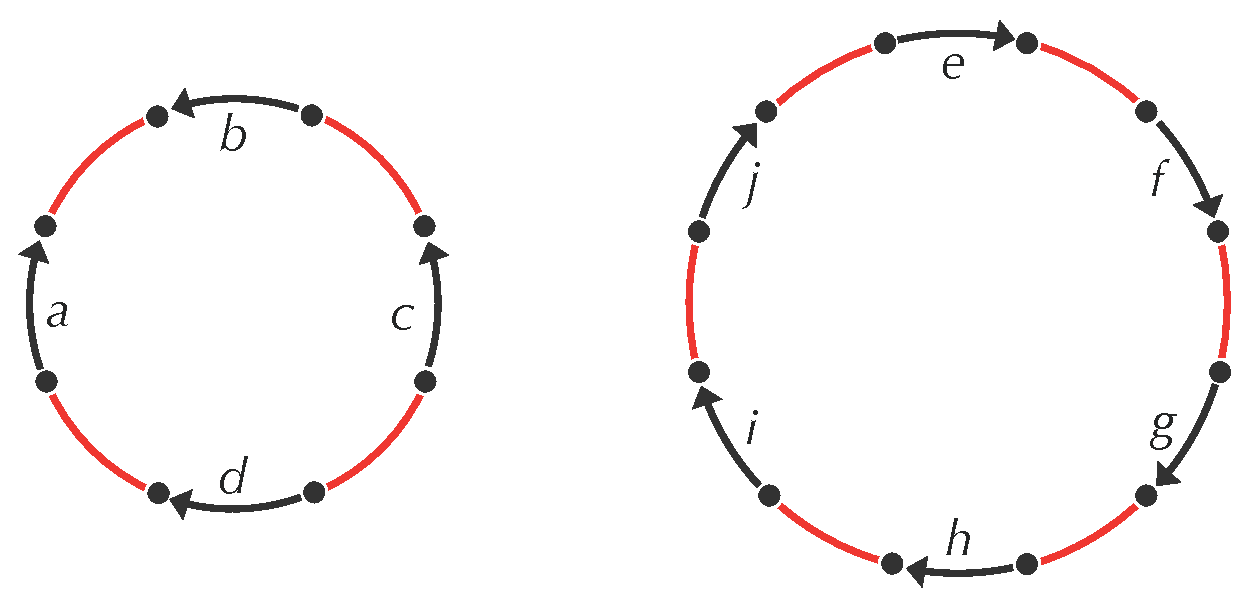
\includegraphics[width = 0.7\textwidth]{images/rearrangements/genome_graph}
\caption{A genome with two circular chromosomes, $(+a$ $-b$ $-c$ $+d)$ and $(+e$ $+f$ $+g$ $+h$ $+i$ $+j)$.  Black directed edges represent synteny blocks, and red undirected edges connect adjacent synteny blocks. A circular chromosome with $n$ elements can be written in $2n$ different ways; the chromosome on the left can be written as $(+a$ $-b$ $-c$ $+d)$, $(-b$ $-c$ $+d$ $+a)$, $(-c$ $+d$ $+a$ $-b)$, $(+d$ $+a$ $-b$ $-c)$, $(-a$ $-d$ $+c$ $+b)$  $(-d$ $+c$ $+b$ $-a)$, $(+c$ $+b$ $-a$ $-d)$, and $(+b$ $-a$ $-d$ $+c)$.}
\label{fig:genome_graph}
\end{figure}

\vspace{\baselineskip}

\begin{qbox}[
Let $P$ and $Q$ be genomes consisting of linear chromosomes, and let $P^{*}$ and $Q^{*}$ be the circularized versions of these genomes. Can you convert a given series of  reversals/translocations/fusions/fissions transforming $P$ into $Q$ into a series of rearrangements transforming $P^{*}$ into $Q^{*}$?  What about the reverse operation --- can you convert a series of rearrangements transforming $P^{*}$ into $Q^{*}$ into a series of rearrangements transforming $P$ into $Q$?
]\end{qbox}

\vspace{-0.5\baselineskip}

\phantomsection
\subsection{2-breaks}
\label{subsec:two-breaks}

We now focus on one of the chromosomes in a multi-chromosomal genome and consider a reversal transforming the circular chromosome $P=(+a$ $-b$ $-c$ $+d)$ into $Q=(+a$ $-b$ $-d$ $+c)$. We can draw $Q$ in a variety of ways, depending on how we choose to arrange its black edges. \autoref{fig:two_equivalent_drawings} shows two such equivalent representations.

\begin{figure}[h]
\mySfFamily
\centering
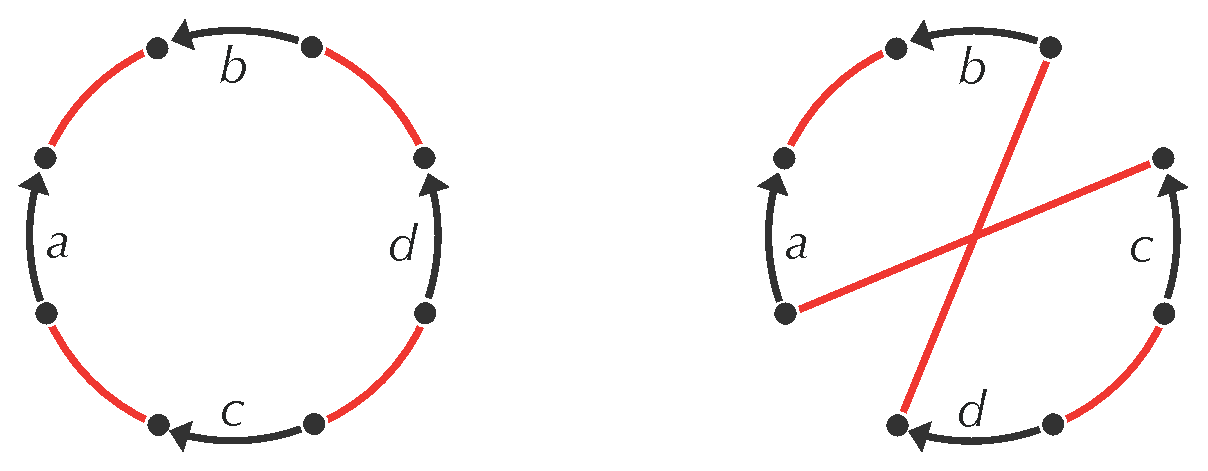
\includegraphics[width = 0.7\textwidth]{images/rearrangements/two_equivalent_drawings}
\caption{Two equivalent drawings of the circular permutation $Q=(+a$ $-b$ $-d$ $+c)$.}
\label{fig:two_equivalent_drawings}
\end{figure}

Although the first drawing of $Q$ in \autoref{fig:two_equivalent_drawings} is its most natural representation, we will use the second representation because its black edges are arranged around the circle in exactly the same order as they appear in the natural representation of $P=(+a$ $-b$ $-c$ $+d)$.  As illustrated in \autoref{fig:genome_reversal}, keeping the black edges fixed allows us to visualize the effect of the reversal.  As you can see, the reversal deletes (``breaks'') two red edges in $P$ (connecting $b$ to $c$ and $d$ to $a$) and replaces them with two new red edges (connecting $b$ to $d$ and $c$ to $a$).\\

\begin{figure}[h]
\mySfFamily
\centering
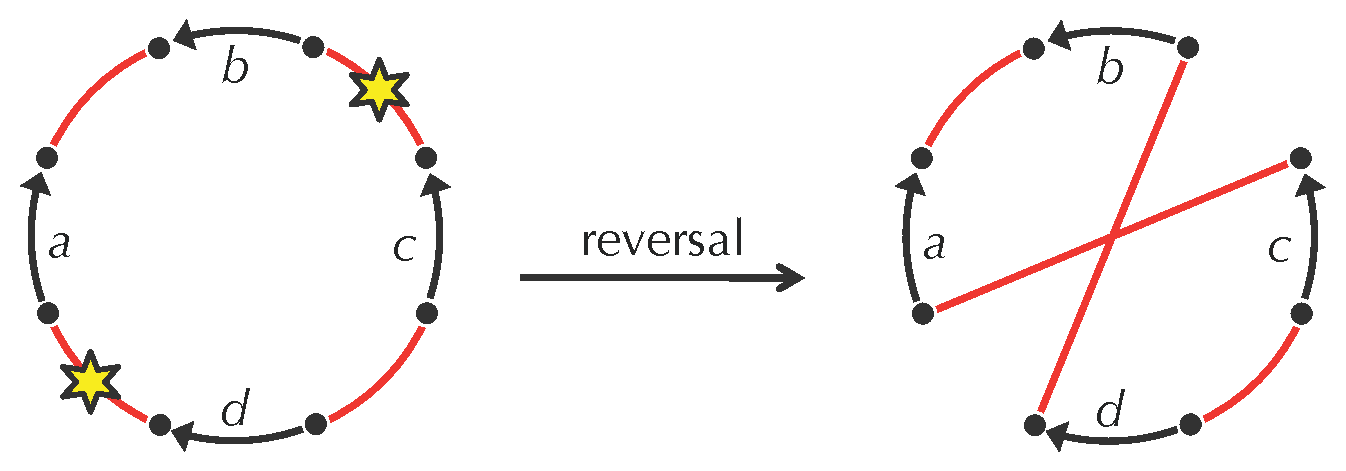
\includegraphics[width = 0.8\textwidth]{images/rearrangements/genome_reversal}
\caption{A reversal transforms $P=(+a$ $-b$ $-c$ $+d)$ into $Q=(+a$ $-b$ $-d$ $+c)$.  We have arranged the black edges of $Q$ so that they have the same orientation and position as the black edges in the natural representation of $P$.  The reversal can be viewed as deleting the two red edges labeled by stars and replacing them with two new red edges on the same four nodes.}
\label{fig:genome_reversal}
\end{figure}

\autoref{fig:fission_and_fusion} illustrates a fission of genome $P=(+a$ $-b$ $-c$ $+d)$ into $Q = (+a$ $-b) (-c$ $+d)$; reversing this operation corresponds to a fusion of the two chromosomes of $Q$ to yield $P$. Both the fusion and the fission operations, like the reversal, correspond to deleting two edges in one genome and replacing them with two new edges in the other genome.

\begin{figure}[h]
\mySfFamily
\centering
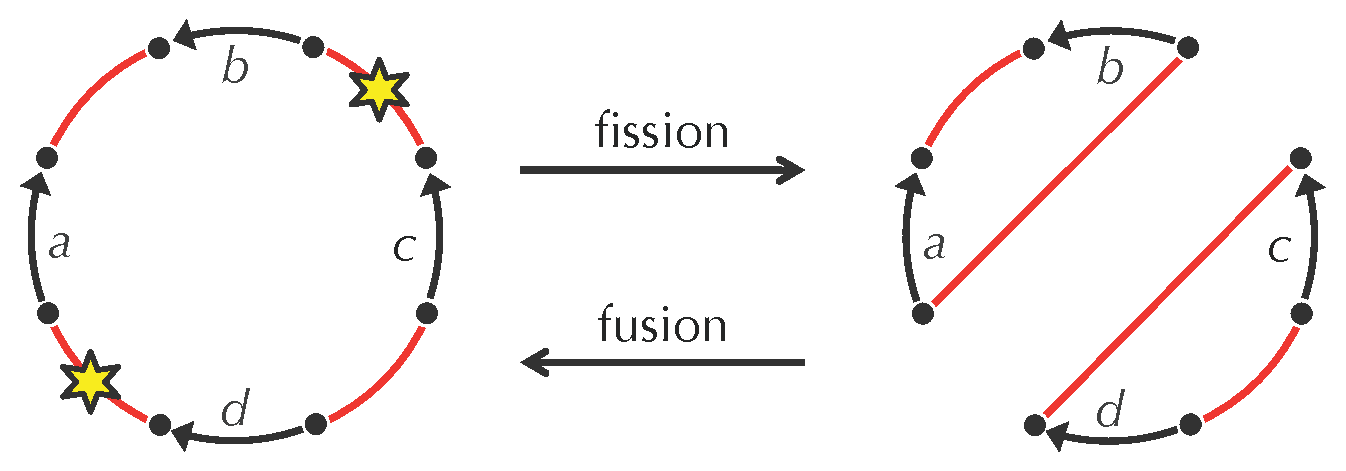
\includegraphics[width = 0.8\textwidth]{images/rearrangements/fission_and_fusion}
\caption{A fission of the single chromosome $P = (+a$ $-b$ $-c$ $+d)$ into the genome $Q = (+a$ $-b)(-c$ $+d)$.  We have again arranged the black edges of $Q$ so that they have the same position and orientation as in the natural representation of $P$.  The inverse operation is a fusion, transforming the two chromosomes of $Q$ into a single chromosome by breaking two red edges of $Q$ and replacing them with two other edges.}
\label{fig:fission_and_fusion}
\end{figure}

A translocation involving two linear chromosomes can also be mimicked by circularizing these chromosomes and then replacing two red edges with two different red edges, as shown in \autoref{fig:translocation}. We have therefore found a common theme uniting the four different types of rearrangements. They all can be viewed as breaking two red edges of the genome graph and replacing them with two new colored edges on the same four nodes.  For this reason, we define the general operation on the genome graph in which two red edges are replaced with two new red edges on the same four nodes as a \textdef{2-break}.

\begin{figure}[h]
\mySfFamily
\centering
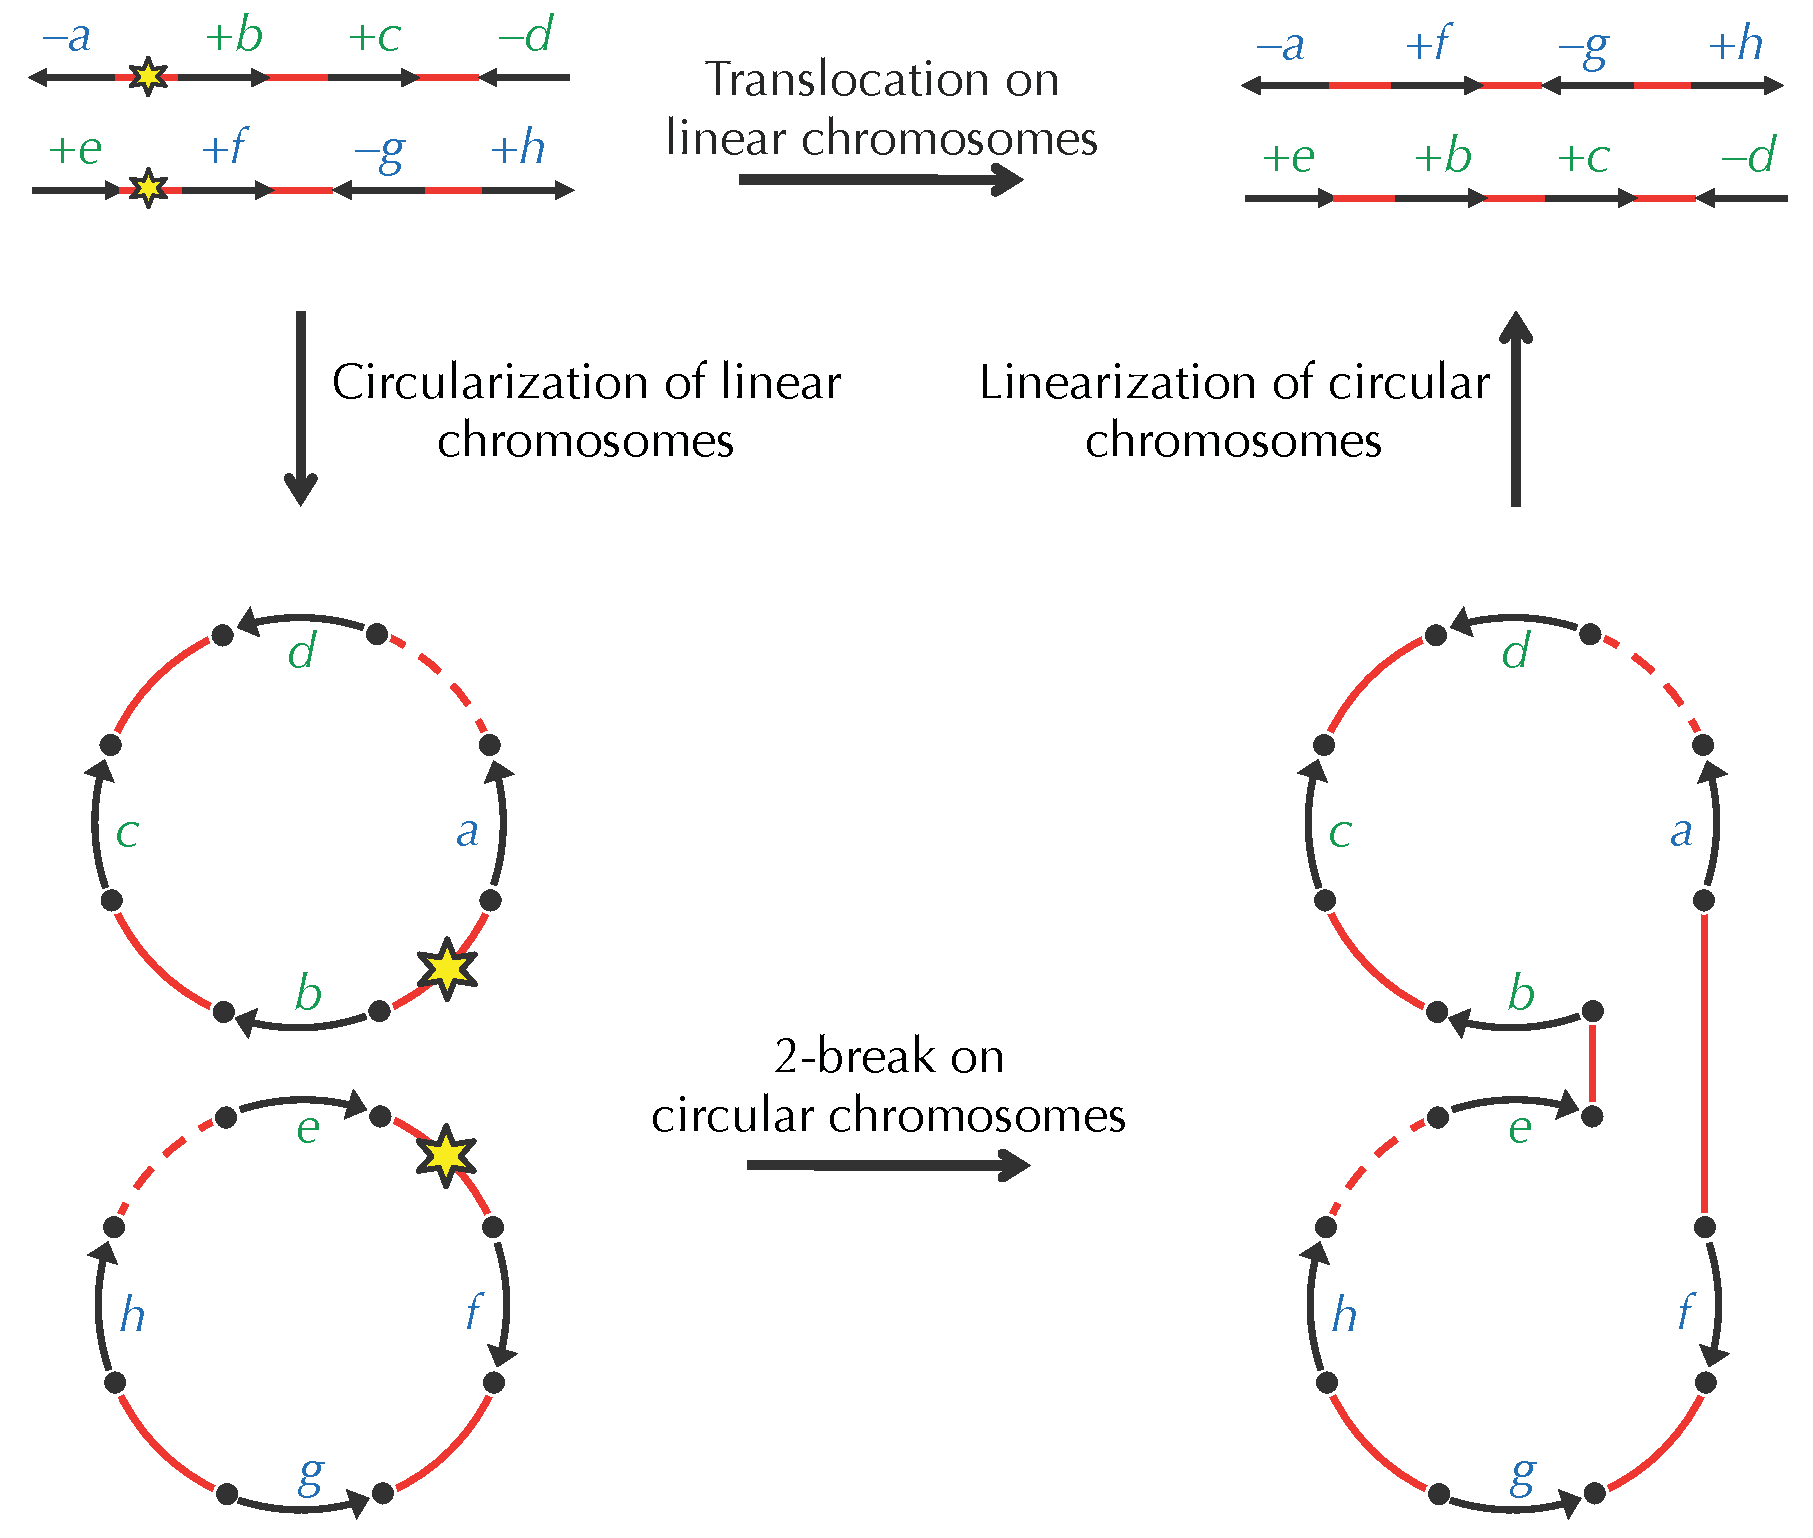
\includegraphics[width = 0.856\textwidth]{images/rearrangements/translocation}
\caption{A translocation of linear chromosomes $(\MathBlue{-a}$ $\MathGreen{+b}$ $\MathGreen{+c}$ $\MathGreen{-d})$  and  $(\MathGreen{+e}$ $\MathBlue{+f}$ $\MathBlue{-g}$ $\MathBlue{+h})$ transforms them into linear chromosomes $(\MathBlue{-a}$ $\MathBlue{+f}$ $\MathBlue{-g}$ $\MathBlue{+h})$ and $(\MathGreen{+e}$ $\MathGreen{+b}$ $\MathGreen{+c}$ $\MathGreen{-d})$. This translocation can also be accomplished by first circularizing the chromosomes, then applying a 2-break to the new chromosomes, and finally converting the resulting circular chromosomes into two linear chromosomes.}
\label{fig:translocation}
\end{figure}

We would like to find a shortest sequence of 2-breaks transforming genome $P$ into genome $Q$, and we refer to the number of operations in this shortest sequence as the \textdef{2-break distance} between $P$ and $Q$, denoted $d(P,Q)$.\\

\begin{problem}[2-Break Distance Problem]{Find the 2-break distance between two genomes.}{Two genomes with circular chromosomes on the same set of synteny blocks.}{The 2-break distance between these genomes.}
\end{problem}

\noindent To compute the 2-break distance, we will return to the notion of breakpoints to construct a graph for comparing two genomes.\\

\phantomsection
\FloatBarrier
\section{Breakpoint Graphs}
\label{sec:breakpoint_graphs}

Consider the genomes $\red{P}=(+a$ $-b$ $-c$ $+d)$ and $\blue{Q} =(+a$ $+c$ $+b$ $-d)$ (\autoref{fig:breakpoint_graph}, left). Note that we have used red for the colored edges of $\red{P}$ and blue for the colored edges of $\blue{Q}$. As before, we rearrange the black edges of $\blue{Q}$ so that they are arranged exactly as in $\red{P}$ (\autoref{fig:breakpoint_graph}, middle). If we superimpose the graphs of $\red{P}$ and $\blue{Q}$, then we obtain the tri-colored \textdef{breakpoint graph} $\textfunc{BreakpointGraph}(\red{P}, \blue{Q})$ (\autoref{fig:breakpoint_graph}, right).

\begin{figure}[h]
\mySfFamily
\centering
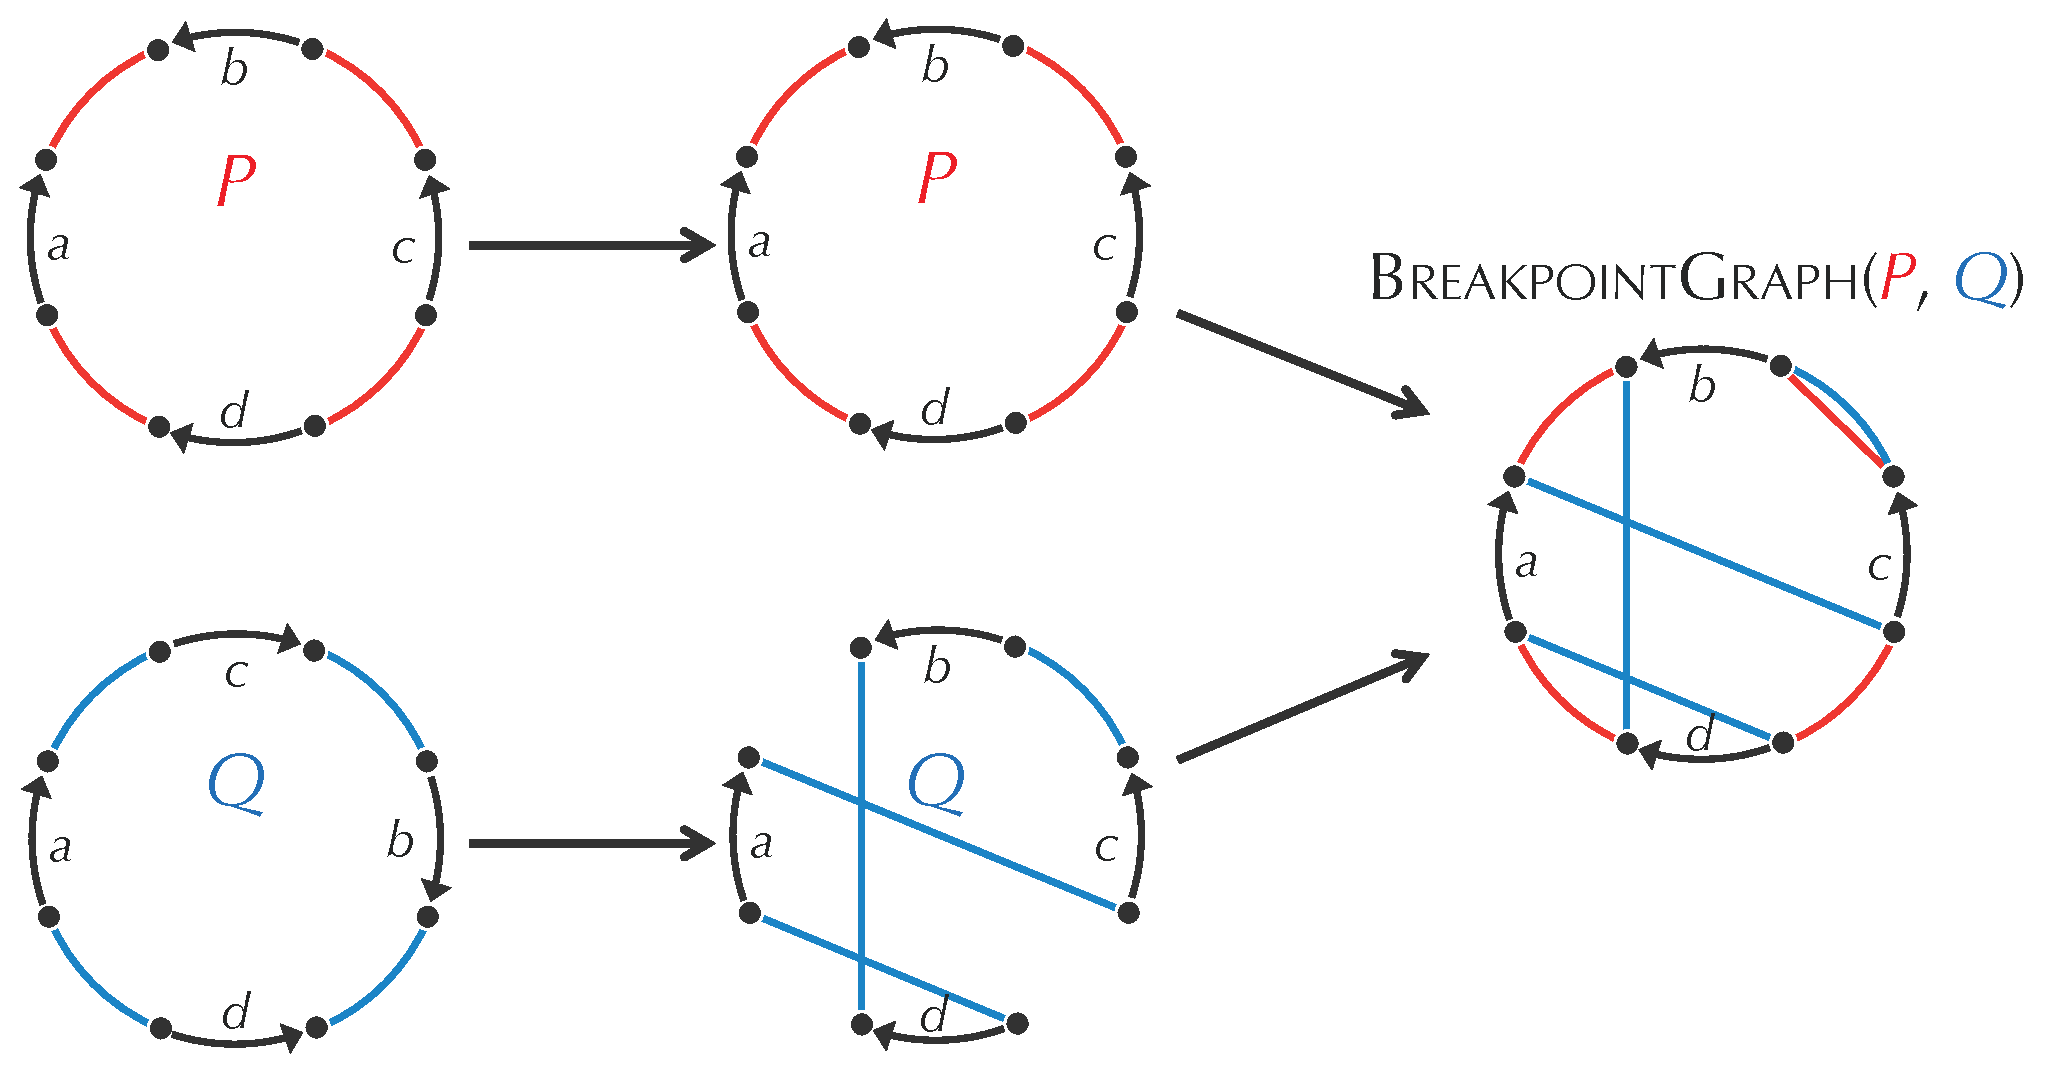
\includegraphics[width = 0.856\textwidth]{images/rearrangements/breakpoint_graph}
\caption{(Left) A red-black genome $\red{P} = (+a ~{-b} ~ {-c} ~ +d)$ and a blue-black genome $\blue{Q} = (+a ~ +c ~ +b ~ {-d})$. (Middle) Rearranging the black edges of $\blue{Q}$ so that they are arranged the same as in $\red{P}$. (Right) The breakpoint graph $\textfunc{BreakpointGraph}(\red{P}, \blue{Q})$, formed by superimposing the graphs of $\red{P}$ and $\blue{Q}$.}
\label{fig:breakpoint_graph}
\end{figure}

Note that the red and black edges in the breakpoint graph form genome $\red{P}$, and the blue and black edges form genome $\blue{Q}$. Moreover, the red and blue edges in the breakpoint graph form a collection of red-blue alternating cycles.\\

\begin{qbox}[
Prove that the red and blue edges in any breakpoint graph form alternating cycles.  Hint: How many red and blue edges meet at each node of the breakpoint graph?
]\end{qbox}

\noindent We denote the number of red-blue alternating cycles in $\textfunc{BreakpointGraph}(\red{P}, \blue{Q})$ as $\textfunc{Cycles}(\red{P}, \blue{Q})$. For $\red{P}=(+a$ $-b$ $-c$ $+d)$ and $\blue{Q} = (+a$ $+c$ $+b$ $-d)$, $\textfunc{Cycles}(\red{P}, \blue{Q}) = 2$, as shown in \autoref{fig:breakpoint_graph_alternating_cycles} (left). In what follows, we will be focusing on the red-blue alternating cycles in breakpoint graphs and often omit the black edges.

\begin{figure}[h]
\mySfFamily
\centering
\begin{tabular}{c @{\hskip 5em} c}
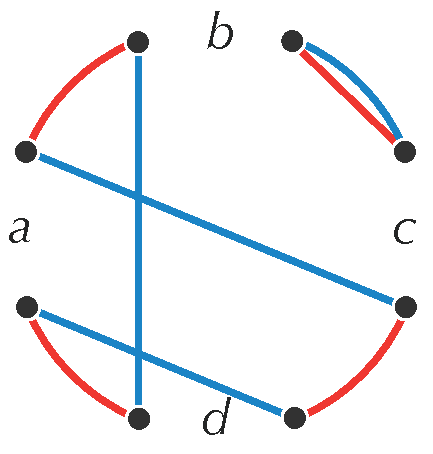
\includegraphics[width = 0.2\textwidth]{images/rearrangements/breakpoint_graph_alternating_cycles} & 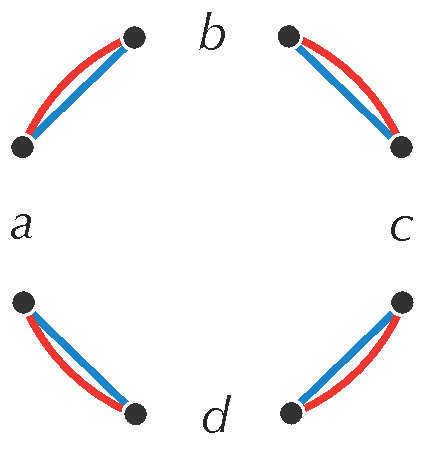
\includegraphics[width = 0.2\textwidth]{images/rearrangements/trivial_breakpoint_graph}
\end{tabular}
\caption{(Left) The red-blue alternating cycles in $\textfunc{BreakpointGraph}(\red{P}, \blue{Q})$ for $\red{P}=(+a$ $-b$ $-c$ $+d)$ and $\blue{Q} = (+a$ $+c$ $+b$ $-d)$. (Right) The trivial breakpoint graph $\textfunc{BreakpointGraph}(\red{P}, \blue{P})$, formed by two copies of the genome $P = (+a$  $-b$ $-c$ $+d)$. The breakpoint graph of \emph{any} genome with itself consists only of trivial (i.e., length 2) alternating cycles.}
\label{fig:breakpoint_graph_alternating_cycles}
\end{figure}

Although \autoref{fig:breakpoint_graph} illustrates the construction of the breakpoint graph for single-chromosomal genomes, the breakpoint graph can be constructed for genomes with multiple chromosomes in exactly the same way (\autoref{fig:breakpoint_graph_multiple_chromosomes}).\\

\begin{figure}[h]
\mySfFamily
\centering
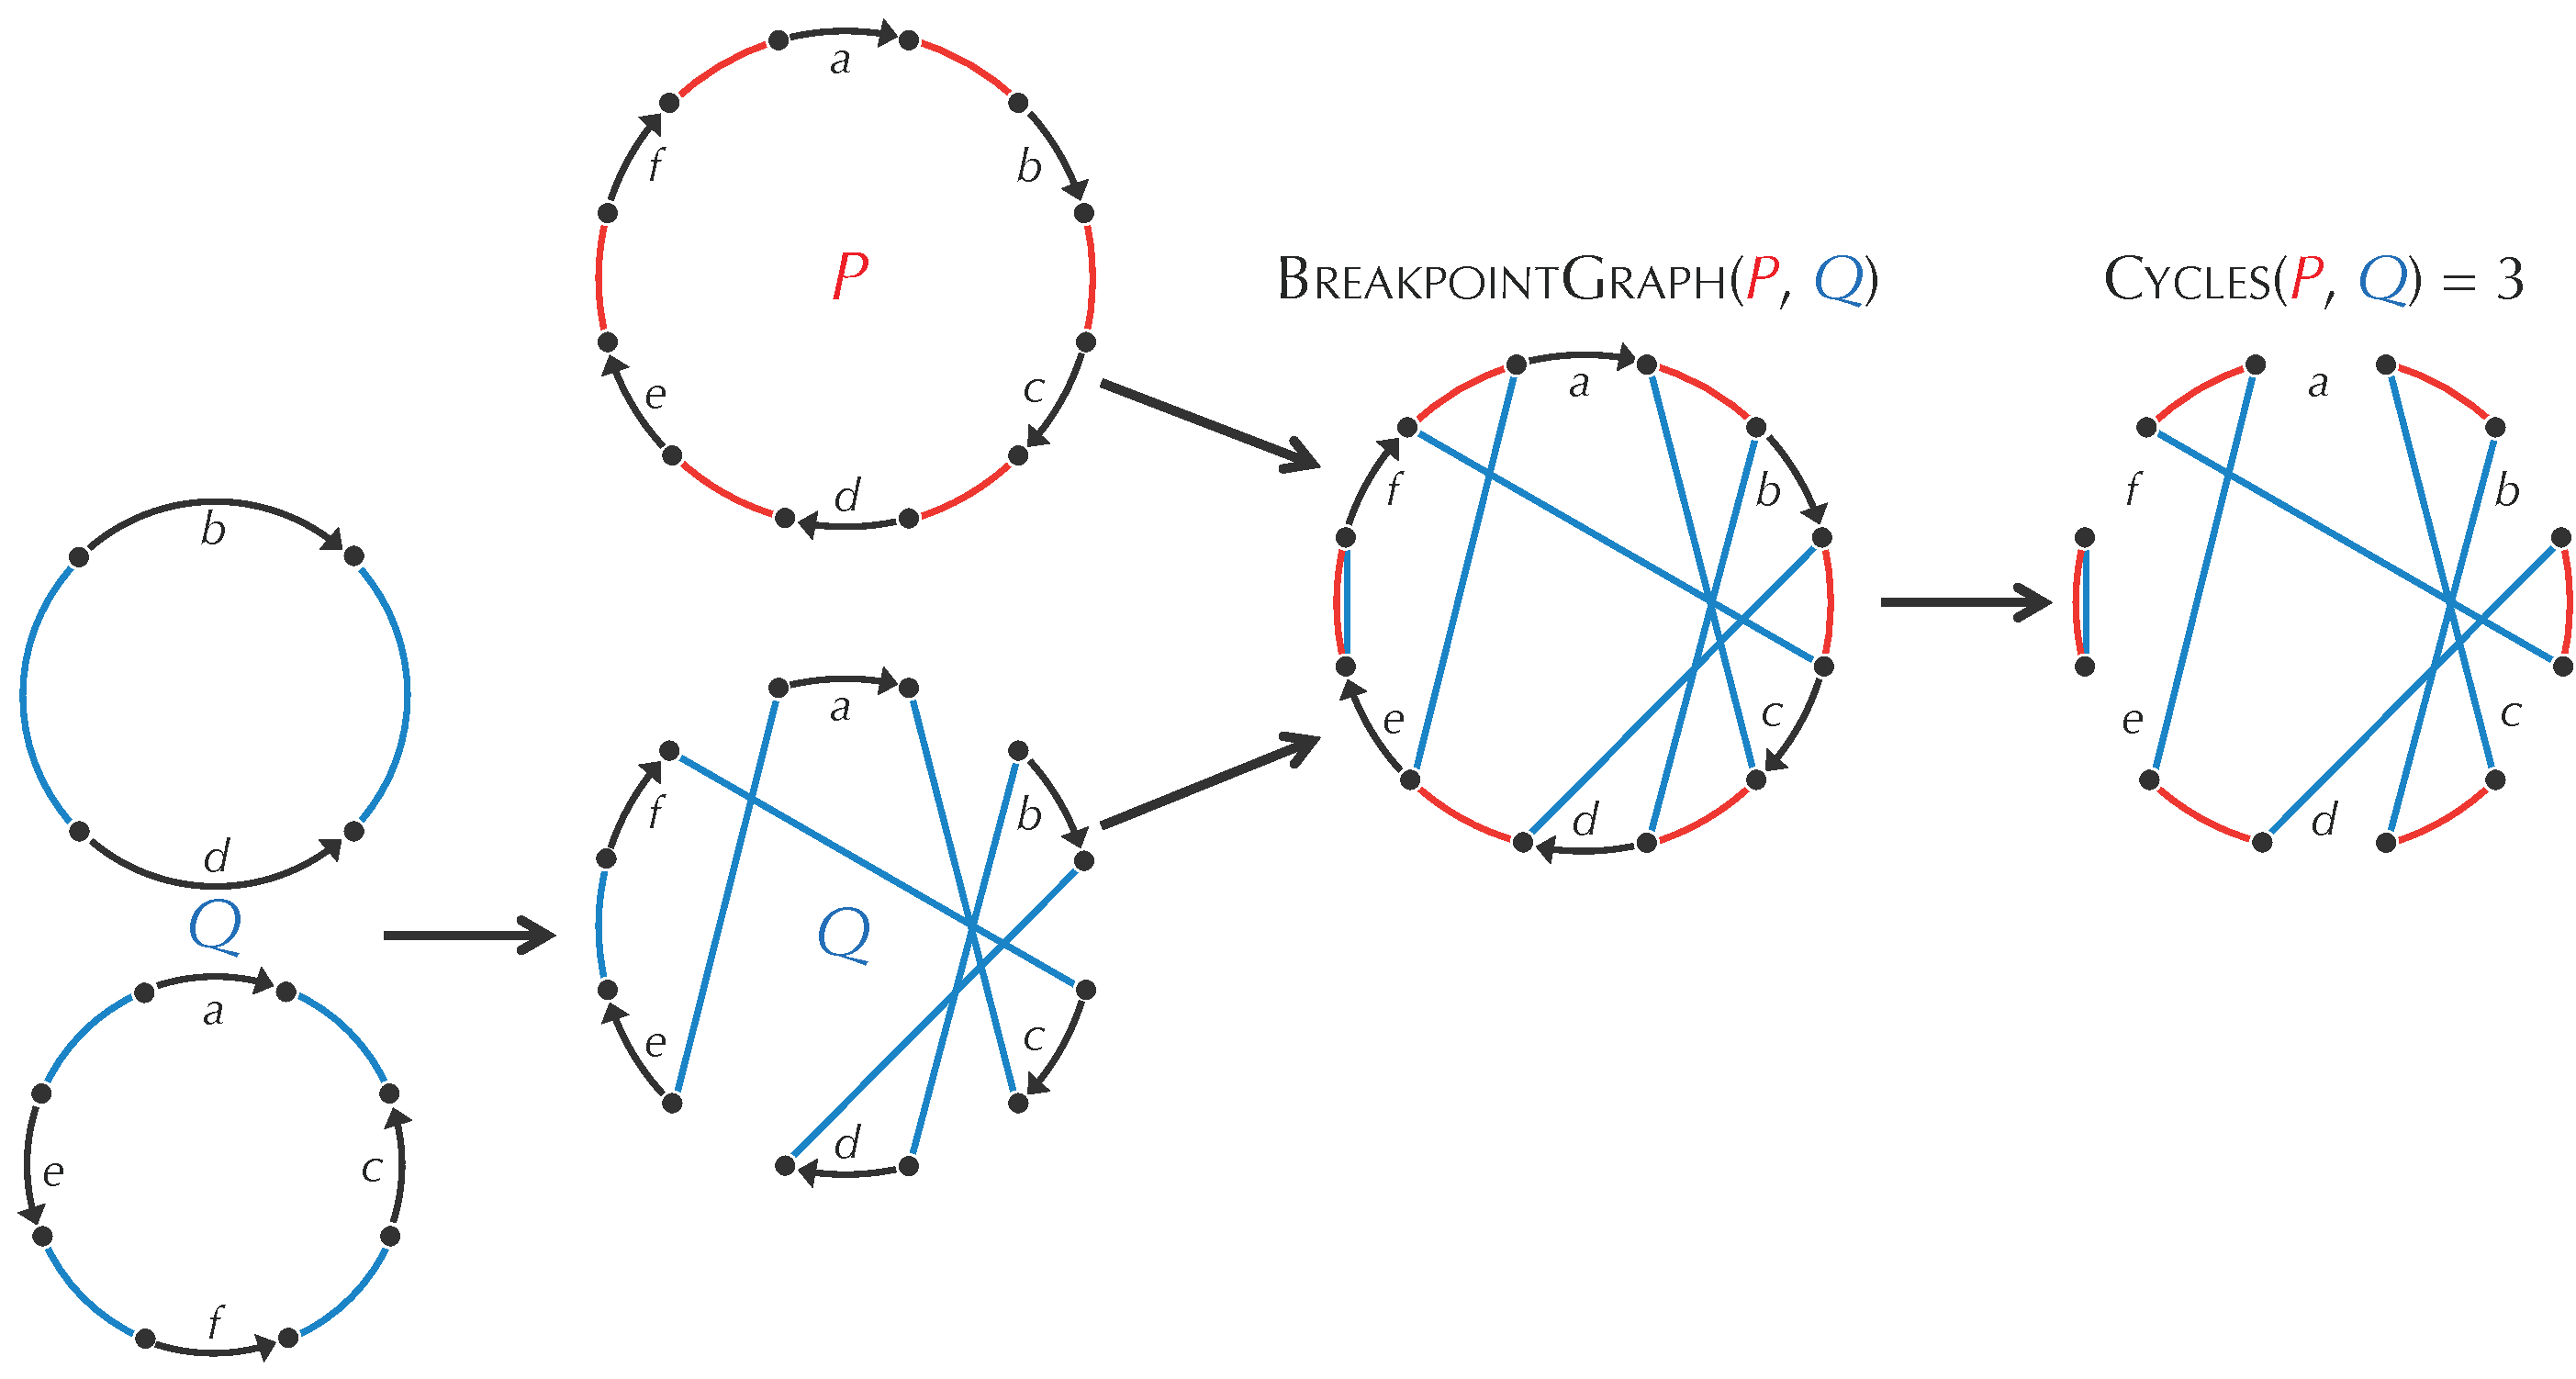
\includegraphics[width = 0.856\textwidth]{images/rearrangements/breakpoint_graph_multiple_chromosomes}
\caption{The construction of $\textfunc{BreakpointGraph}(\red{P}, \blue{Q})$ for the unichromosomal genome $\red{P} = (+a$ $+b$ $+c$ $+d$ $+e$ $+f)$ and the two-chromosome genome $\blue{Q} = (+a$  $-c$ $-f$ $-e)(+b$ $-d)$. At the bottom, to illustrate the construction of the breakpoint graph, we first rearrange the black edges of $\blue{Q}$ so that they are drawn the same as in $\red{P}$.}
\label{fig:breakpoint_graph_multiple_chromosomes}
\end{figure}

\begin{qbox}[
Given genome $\red{P}$, which genome $\blue{Q}$ maximizes $\textfunc{Cycles}(\red{P}, \blue{Q})$?
]\end{qbox}

\vspace{-0.5\baselineskip}

\noindent We denote the number of synteny blocks shared by genomes $\red{P}$ and $\blue{Q}$ as $\textfunc{Blocks}(\red{P}, \blue{Q})$.  As shown in \autoref{fig:breakpoint_graph_alternating_cycles} (right), when $\red{P}$ and $\blue{Q}$ are identical, their breakpoint graph consists of $\textfunc{Blocks}(\red{P}, \blue{Q})$  cycles of length 2, each containing one red and one blue edge. We refer to cycles of length 2 as \textdef{trivial cycles} and the breakpoint graph formed by identical genomes as the \textdef{trivial breakpoint graph}.

%\begin{figure}[h]
%\mySfFamily
%\centering
%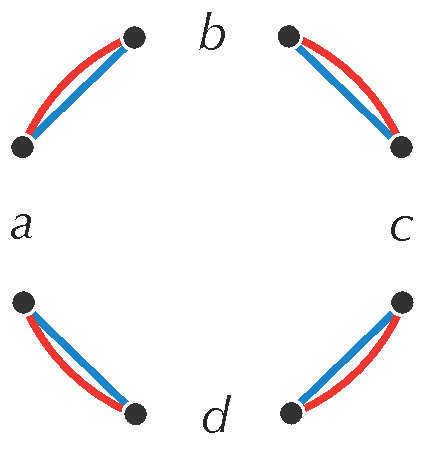
\includegraphics[width = 0.2\textwidth]{images/rearrangements/trivial_breakpoint_graph}
%\caption{The trivial breakpoint graph $\textfunc{BreakpointGraph}(\red{Q}, \blue{Q})$ formed by two copies of the genome $Q = (+a$  $-b$ $-c$ $+d)$.}
%\label{fig:trivial_breakpoint_graph}
%\end{figure}

You are likely wondering how the breakpoint graph is useful. We can view a 2-break transforming $\red{P}$ into $\red{P'}$ as an operation on $\textfunc{BreakpointGraph}(\red{P}, \blue{Q})$ that yields $\textfunc{BreakpointGraph}(\red{P'}\hspace{-0.1em}, \blue{Q})$ (\autoref{fig:2_break_breakpoint_graph}).

By extension, we can view a series of 2-breaks transforming $\red{P}$ into $\blue{Q}$ as a series of 2-breaks transforming $\textfunc{BreakpointGraph}(\red{P}, \blue{Q})$ into $\textfunc{BreakpointGraph}(\red{Q}, \blue{Q})$, the trivial breakpoint graph (\autoref{fig:2_break_series}).  \autoref{fig:2_break_series_example} illustrates a transformation of a breakpoint graph with $\textfunc{Cycles}(\red{P}, \blue{Q}) = 2$ into a trivial breakpoint graph with $\textfunc{Cycles}(\red{Q}, \blue{Q}) = 4$ using two 2-breaks.\par

\begin{figure}[h]
\mySfFamily
\centering
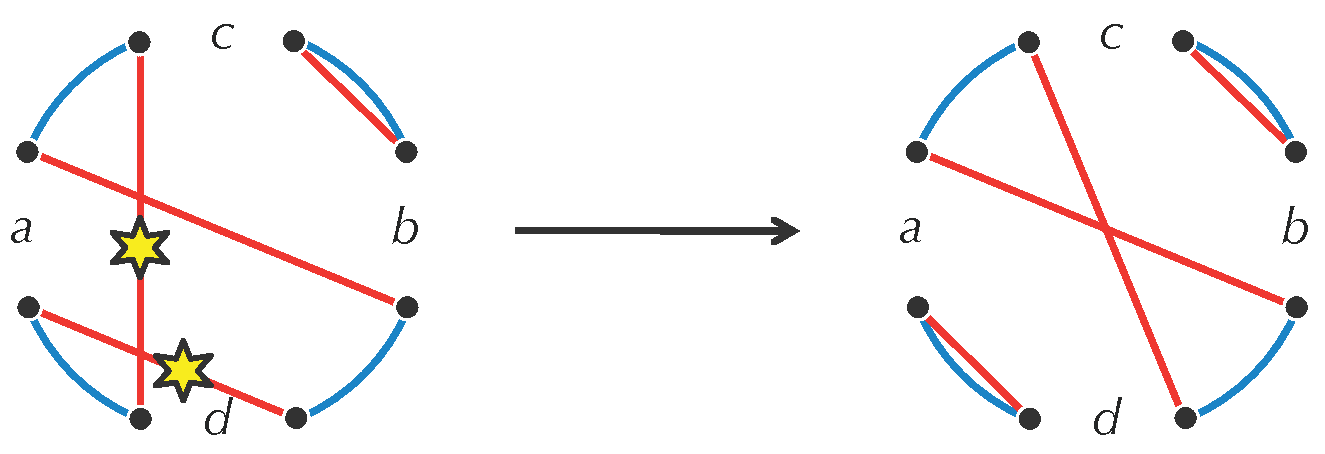
\includegraphics[width = 0.6\textwidth]{images/rearrangements/2-break_breakpoint_graph}
\caption{A 2-break transforming genome $\red{P}$ into genome $\red{P'}$ also transforms $\textfunc{BreakpointGraph}(\red{P}, \blue{Q})$ into  $\textfunc{BreakpointGraph}(\red{P'}\hspace{-0.1em}, \blue{Q})$ for any permutation $\blue{Q}$.}
\label{fig:2_break_breakpoint_graph}
\end{figure}

\begin{figure}[h]
\mySfFamily
\centering
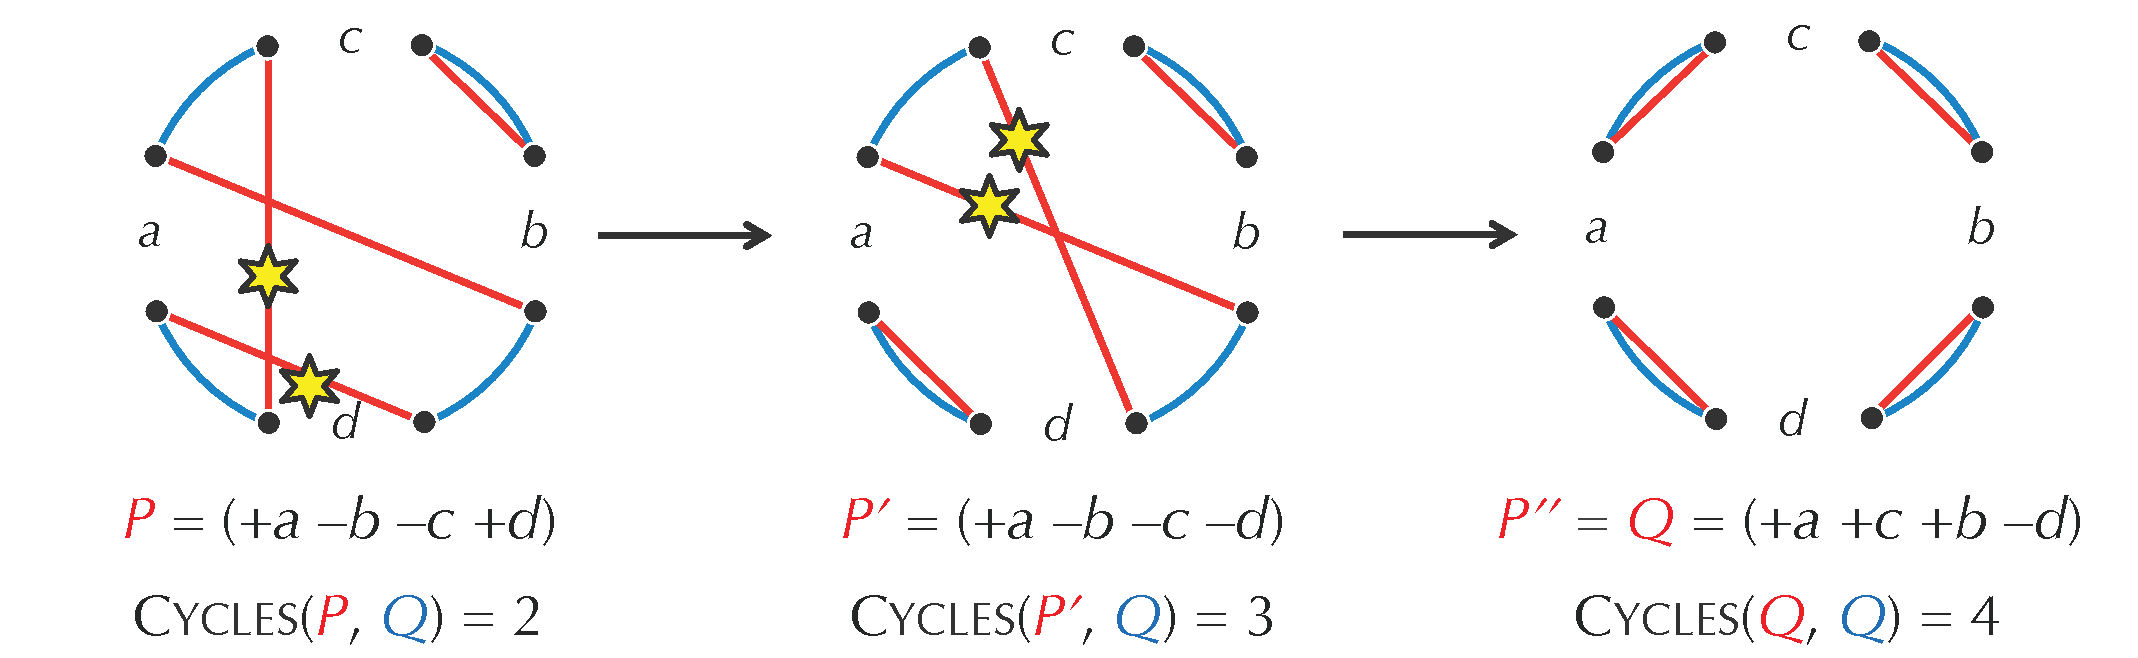
\includegraphics[width = 0.856\textwidth]{images/rearrangements/2-break_series}
\caption{Every 2-break transformation of $\red{P}$ into $\blue{Q}$ corresponds to a transformation of $\textfunc{BreakpointGraph}(\red{P}, \blue{Q})$ into $\textfunc{BreakpointGraph}(\red{Q}, \blue{Q})$. In the example shown, the number of red-blue cycles in the graph increases from $\textfunc{Cycles}(\red{P}, \blue{Q}) = 2$ to $\textfunc{BreakpointGraph}(\red{Q}, \blue{Q}) = \textfunc{Blocks}(\red{Q}, \blue{Q}) = 4$.}
\label{fig:2_break_series}
\end{figure}

\begin{figure}[h]
\mySfFamily
\centering
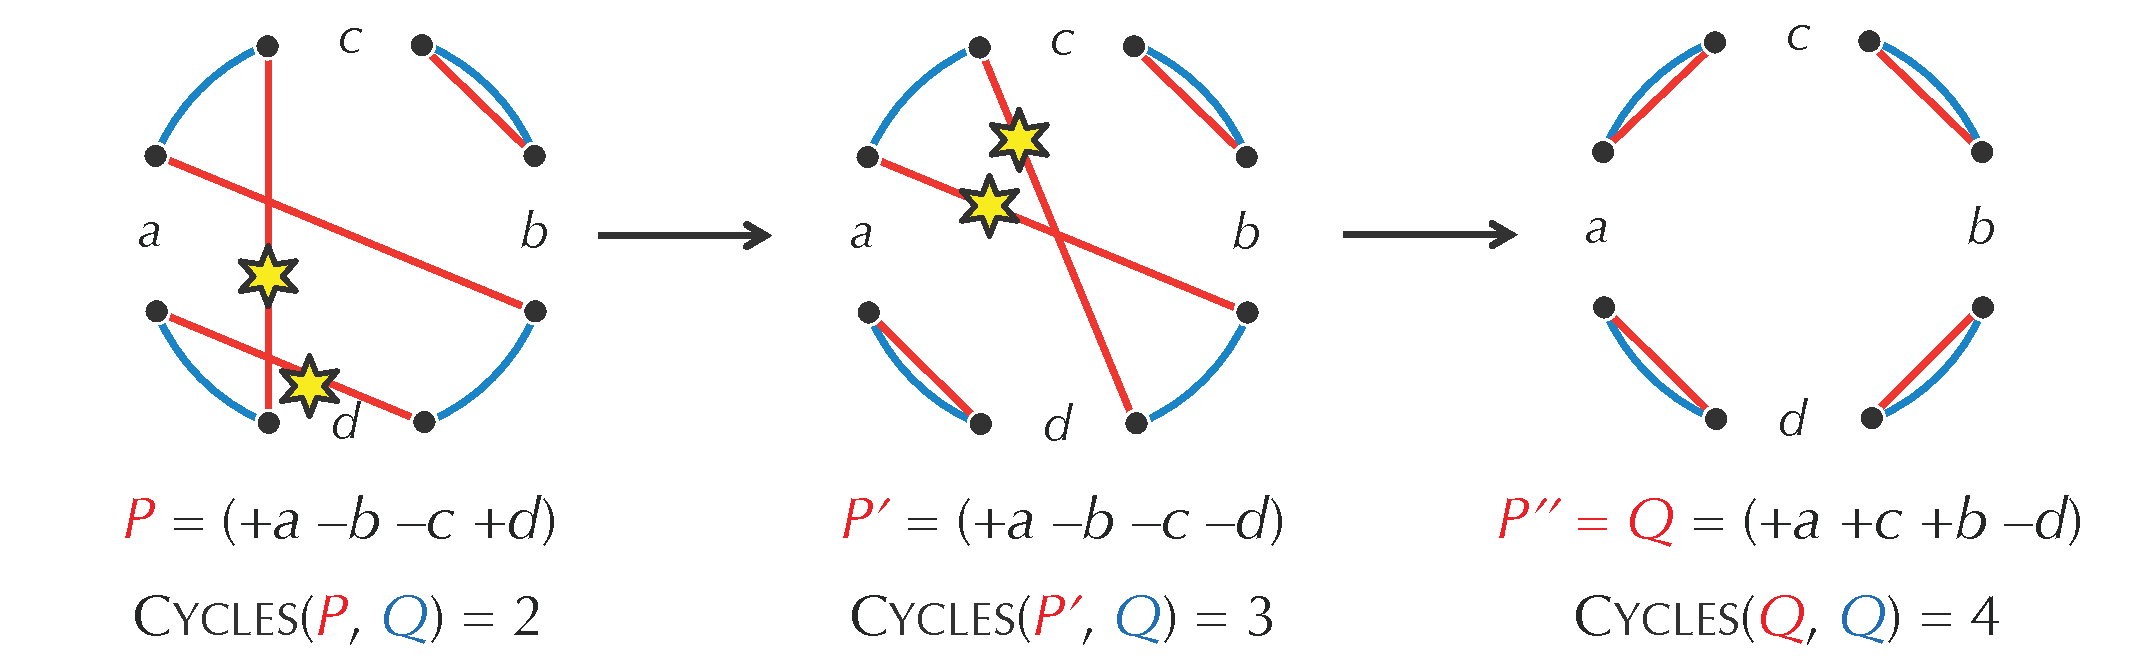
\includegraphics[width = 0.856\textwidth]{images/rearrangements/2-break_series_example}
\caption{The transformation $\red{P} \rightarrow \red{P'} \rightarrow \red{Q}$ induces a transformation of the breakpoint graph $\textfunc{BreakpointGraph}(\red{P}, \blue{Q})$ with 2 alternating cycles into the trivial breakpoint graph.  Stars indicate red edges that are replaced in a 2-break.}
\label{fig:2_break_series_example}
\end{figure}



Since every transformation of $\red{P}$ into $\blue{Q}$ transforms  $\textfunc{BreakpointGraph}(\red{P}, \blue{Q})$ into the trivial breakpoint graph $\textfunc{BreakpointGraph}(\red{Q}, \blue{Q})$, any sorting by 2-breaks increases the number of red-blue cycles by

\begin{center}
$\textfunc{Cycles}(\red{Q}, \blue{Q}) - \textfunc{Cycles}(\red{P}, \blue{Q}) = \textfunc{Blocks}(\red{P}, \blue{Q}) - \textfunc{Cycles}(\red{P}, \blue{Q})$.
\end{center}

\fudgespace

\begin{qbox}[
How much can each individual 2-break contribute to this increase? In other words, if $\red{P'}$ is obtained from $\red{P}$ by a 2-break, how much bigger can $\textfunc{Cycles}(\red{P'}, \blue{Q}) $ be than $\textfunc{Cycles}(\red{P}, \blue{Q})$?
]\end{qbox}

\phantomsection
\FloatBarrier
\section{Computing the 2-Break Distance}
\label{sec:computing_the_2-break_distance}

The Breakpoint Theorem stated that a reversal applied to a linear chromosome $P$ can reduce $\textfunc{Breakpoints}(P)$ by at most 2.  We now prove that a 2-break applied to a multichromosomal genome $P$ can increase $\textfunc{Cycles}(P, Q)$ by at most 1, i.e., for any 2-break transforming $P$ into $P'$, and for any genome $Q$, $\textfunc{Cycles}(P', Q)$ cannot exceed $\textfunc{Cycles}(P, Q) + 1$.

\begin{namedtheorem}[Cycle]
For genomes $P$ and $Q$, any 2-break applied to $P$ can increase $\textfunc{Cycles}(P, Q)$ by at most 1. 
\end{namedtheorem}

\begin{proof}
\autoref{fig:cycle_theorem_proof} presents three cases that illustrate how a 2-break applied to $P$ can affect the breakpoint graph. Each 2-break affects two red edges that either belong to the same cycle or to two different cycles in $\textfunc{BreakpointGraph}(P, Q)$. In the former case, the 2-break either does not change $\textfunc{Cycles}(P, Q)$, or it increases it by 1. In the latter case, it decreases $\textfunc{Cycles}(P, Q)$ by 1.
\end{proof}

\begin{figure}[h]
\mySfFamily
\centering
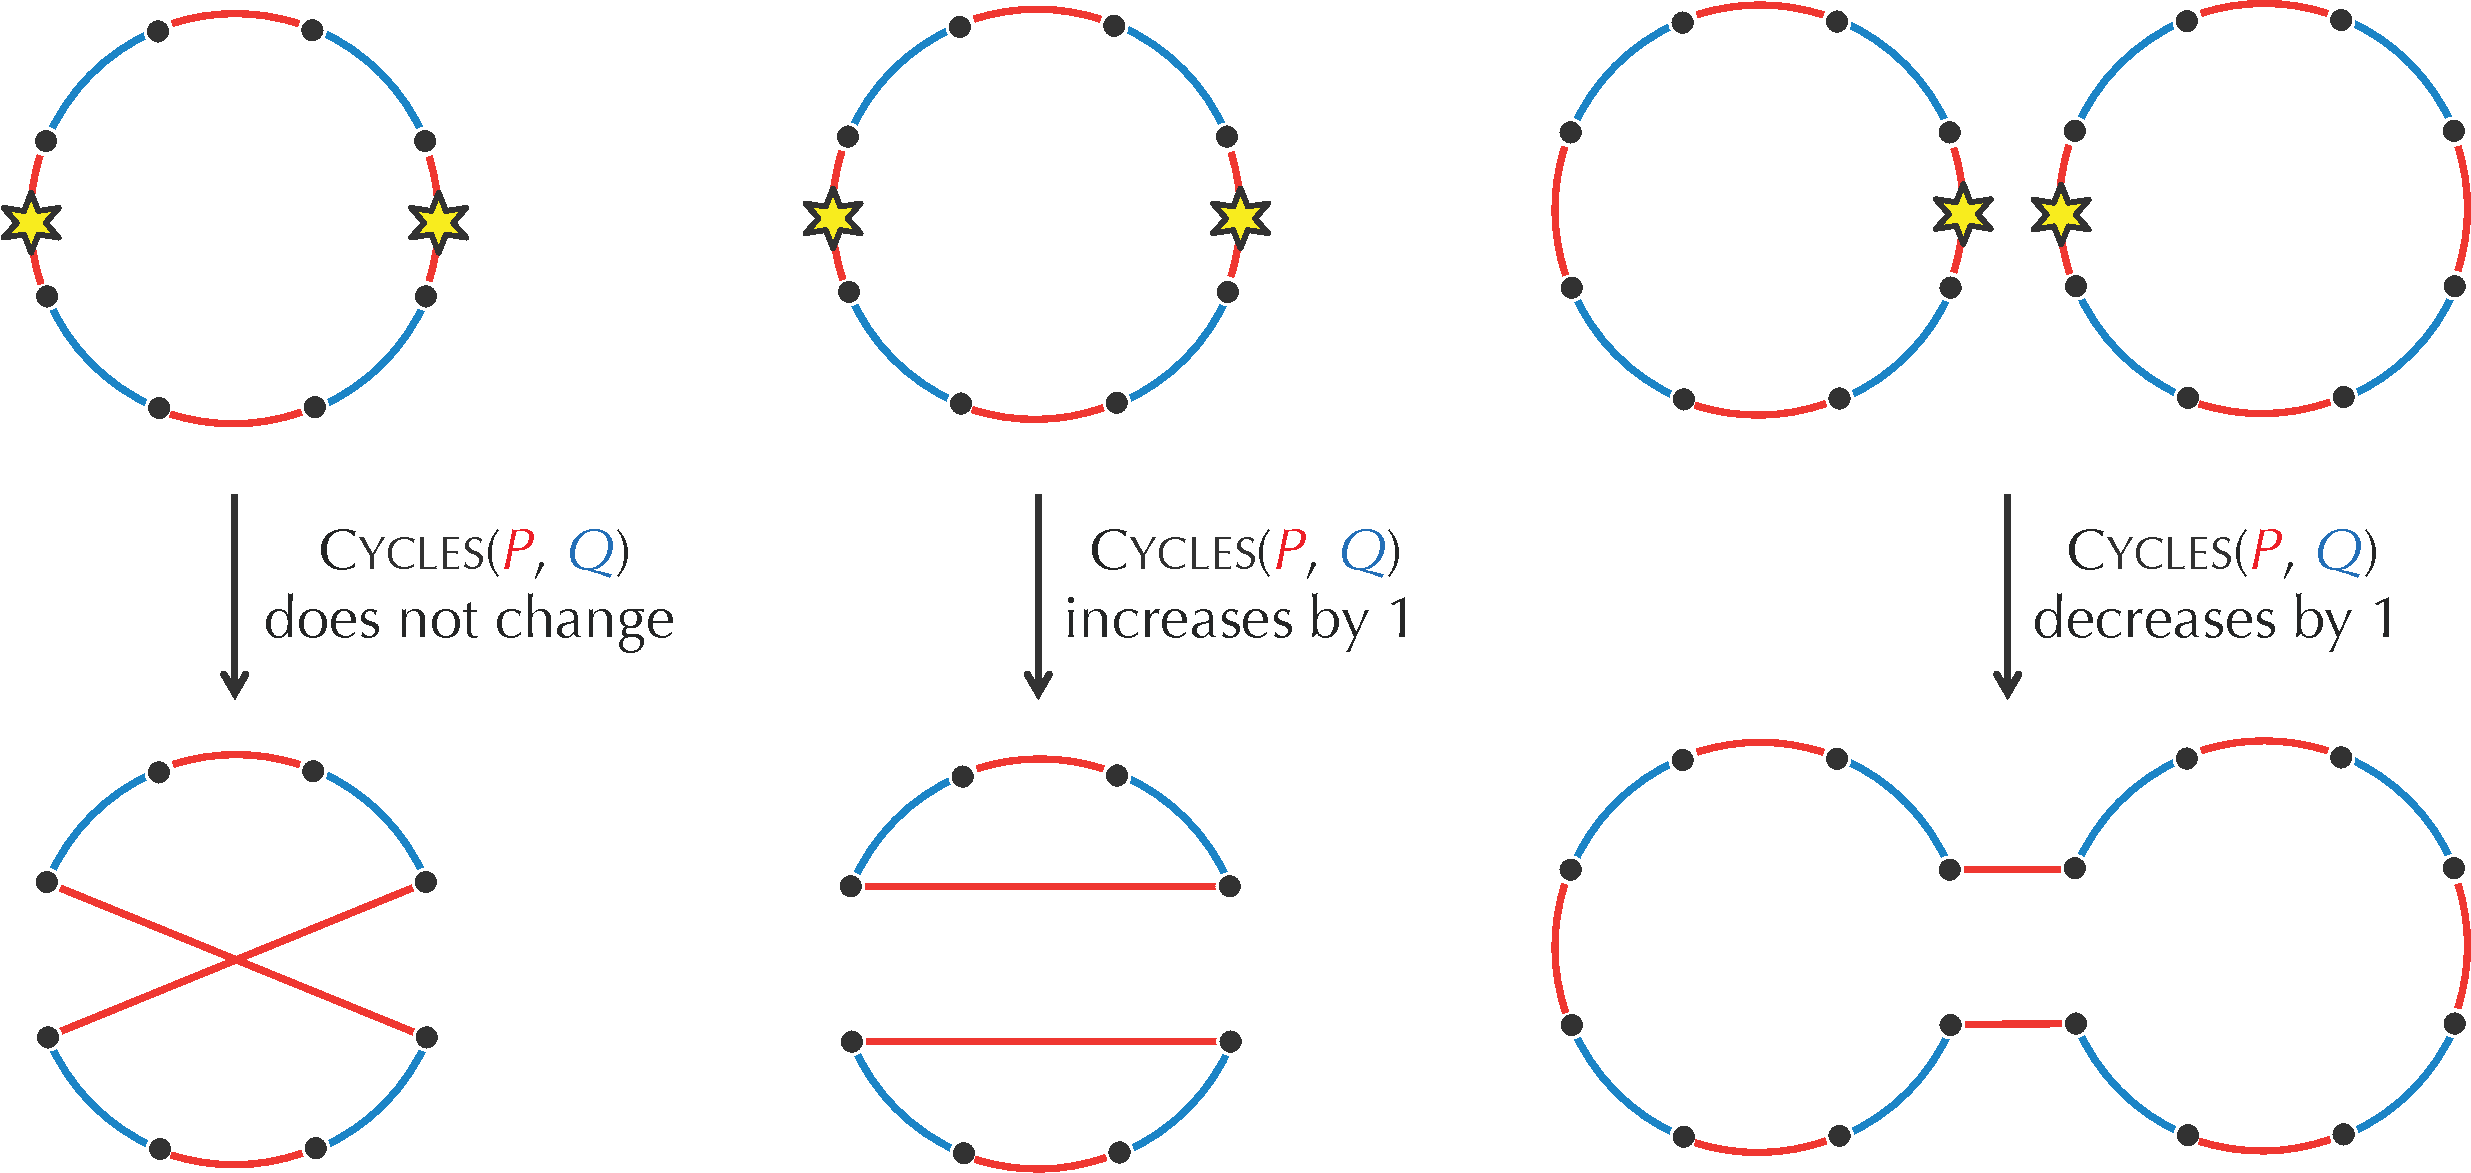
\includegraphics[width = 0.856\textwidth]{images/rearrangements/cycle_theorem_proof}
\caption{Three cases illustrating how a 2-break can affect the breakpoint graph.}
\label{fig:cycle_theorem_proof}
\end{figure}

Although the preceding proof is short and intuitive, it is not a formal proof, but rather an invitation to examine \autoref{fig:cycle_theorem_proof}. If you are interested in a more rigorous mathematical argument, please read the next proof.

\begin{proof}
A 2-break adds 2 new red edges and thus forms at most \textbf{2} new cycles (containing two new red edges) in $\textfunc{BreakpointGraph}(P, Q)$.  At the same time, it breaks 2 red edges and thus removes at least \textbf{1} old cycle (containing two old edges) from $\textfunc{BreakpointGraph}(P, Q)$.  Thus, the number of red-blue cycles in the breakpoint graph increases by at most $\textbf{2} - \textbf{1} = 1$, implying that $\textfunc{Cycles}(P, Q)$ increases by at most 1.
\end{proof}

Recall that there are permutations for which the number of breakpoints cannot be reduced, a fact that defeated our hopes for a greedy algorithm for sorting by reversals that reduces the number of breakpoints at each step. In the case of 2-breaks (on genomes with circular chromosomes), we now know that each 2-break can increase $\textfunc{Cycles}(P, Q)$ by at most 1. But is it \emph{always} possible to find a 2-break that increases $\textfunc{Cycles}(P, Q)$ by 1? The answer, perhaps surprisingly, is yes.

\begin{namedtheorem}[2-Break Distance]
The 2-break distance between genomes $P$ and $Q$ is equal to $\textfunc{Blocks}(P, Q) - \textfunc{Cycles}(P, Q)$.
\end{namedtheorem}

\begin{proof}
Recall that every sorting by 2-breaks must increase the number of alternating cycles by $\textfunc{Blocks}(P, Q) - \textfunc{Cycles}(P, Q)$. The Cycle Theorem implies that each 2-break increases the number of cycles in the breakpoint graph by at most 1.  This immediately implies in turn that $d(P, Q)$ is \emph{at least} $\textfunc{Blocks}(P, Q) - \textfunc{Cycles}(P, Q)$. If $P$ is not equal to $Q$, there must be a non-trivial cycle in $\textfunc{Blocks}(P, Q)$, i.e., a cycle with more than 2 edges. As shown in \autoref{fig:cycle_theorem_proof} (middle), any non-trivial cycle in the breakpoint graph can be split into two cycles by a 2-break, implying that we can always find a 2-break increasing the number of red-blue cycles by 1. Therefore, $d(P,Q)$ is equal to $\textfunc{Blocks}(P, Q) - \textfunc{Cycles}(P, Q)$.
\end{proof}

\protect\computationalproblem[2-Break Distance Problem]{0.8}
Armed with this theorem, you should be ready to design an algorithm solving the 2-Break Distance Problem. Furthermore, having proved the formula $d(P,Q) = \textfunc{Blocks}(P, Q) - \textfunc{Cycles}(P, Q)$ for the 2-break distance between genomes with multiple circular chromosomes, we wonder whether we can find an analogous formula for the reversal distance between single linear chromosomes.\par

\vspace{\baselineskip}

\begin{qbox}[
Compute the 2-break distance between the circularized human and mouse X chromosomes. Can you transform a series of 2-breaks for circularized chromosomes into a series of reversals sorting the linear X chromosomes?
]\end{qbox}

\noindent Perhaps surprisingly, a fast algorithm for sorting permutations by reversals does exist, yielding an exact formula for the reversal distance!  Although this sorting algorithm relies on the notion of breakpoints, it is unfortunately too complicated to present here (see \takedetour[Similar Problems with Different Fates]{similar_problems_with_different_fates}).

The breakpoint graph constructed on the 280 human-mouse synteny blocks contains 35 alternating cycles, so that the 2-break distance between these genomes is $280 - 35 = 245$.  Again, we don't know exactly how many 2-breaks happened in the last 75 million years, but we are certain that there were \emph{at least} 245 steps. Remember this fact, since it will prove important in the next section.\\

\phantomsection
\FloatBarrier
\section{Rearrangement Hotspots in the Human Genome}
\label{sec:rearrangement_hotspots_in_the_human_genome}

\phantomsection
\subsection{The Random Breakage Model meets the 2-Break Distance Theorem}
\label{subsec:the_random_breakage_model_meets_the_2-break_distance_theorem}

You have probably anticipated from the beginning of the chapter that we would eventually argue against the Random Breakage Model.  But it may still be unclear to you how the 2-break distance could possibly be used to do so.

\begin{namedtheorem}[Rearrangement Hotspots]
There are rearrangement hotspots in the human \linebreak genome. 
\end{namedtheorem}

\begin{proof}
Recall that if the Random Breakage Model is correct, then $N$ reversals applied to a linear chromosome will produce approximately $2N + 1$ synteny blocks, since the probability is very low that two nearby locations in the genome will be used as the breakage point of more than one reversal. Similarly, $N$ random 2-breaks applied to circular chromosomes will produce $2N$ synteny blocks. Since there are 280 human-mouse synteny blocks, there must have been approximately $\left. 280 \middle/ 2 = 140 \right.$ 2-breaks on the evolutionary path between humans and mice. However, the 2-Break Distance Theorem tells us that there were at least 245 2-breaks on this evolutionary path.\\

\begin{qbox}[
Is $245 \approx 140$?
]\end{qbox}

\vspace{-0.5\baselineskip}

\noindent Since 245 is much larger than 140, we have arrived at a contradiction, implying that one of our assumptions is incorrect! But the only assumption we made in this proof was ``\emph{If the Random Breakage Model is correct\ldots}'' Thus, this assumption must have been wrong.
\end{proof}

This argument, which is not a mathematical proof, is nevertheless logically solid.  It offers an example of a \textdef{proof by contradiction}, in which we begin by assuming the statement that we intend to disprove and then demonstrate how this assumption leads to a contradiction. As a result of the Rearrangement Hotspots Theorem, we conclude that there was breakpoint reuse on the human-mouse evolutionary path.  This breakpoint reuse was extensive, as quantified by the large ratio between the actual 2-break distance and what the 2-break distance would have been under the Random Breakage Model ($\left. 245 \middle/ 140 = 1.75 \right.$).

Of course, our arguments need to be made statistically sound in order to ensure that the discrepancy between the Random Breakage Model's prediction and the 2-break distance is significant.  After all, even though genomes are large, there is still a small chance that randomly chosen 2-breaks might occasionally break a genome more than once in a small interval.  Unfortunately, the necessary statistical analysis is beyond the scope of this chapter.

\phantomsection
\subsection{The Fragile Breakage Model}
\label{subsec:the_fragile_breakage_model}

But wait --- what about Nadeau and Taylor's argument in favor of the Random Breakage Model?  We certainly cannot ignore that the lengths of the human-mouse synteny blocks resemble an exponential distribution.\\

\begin{qbox}[
Can you find anything wrong with Nadeau and Taylor's logic?
]\end{qbox}

\noindent The Nadeau and Taylor argument in favor of the Random Breakage Model exemplifies a classic logic fallacy.  It is true that if breakage is random, then the histogram of synteny block lengths should follow the exponential distribution. But it is a completely different statement to conclude that just because synteny block lengths follow the exponential distribution, breakage must have been random.  The distribution of synteny block lengths certainly provides support for the Random Breakage Model, but it does not prove that it is correct.

Nevertheless, any alternative hypothesis we put forth for the Random Breakage Model must account for the observation that the distribution of synteny block lengths for the human and mouse genomes is approximately exponential.\\

\begin{qbox}[
Can you propose a different model of chromosome evolution that explains rearrangement hotspots and is consistent with the exponential distribution of synteny block lengths?
]\end{qbox}

\noindent The contradiction of the Random Breakage Model led to an alternative \textdef{Fragile Breakage Model} of chromosome evolution, which was proposed in 2003.  This model states that every mammalian genome is a mosaic of long solid regions, which are rarely affected by rearrangements, as well as short \textdef{fragile regions} that serve as rearrangement hotspots and that account only for a small fraction of the genome.  For humans and mice, these fragile regions make up approximately 3\% of the genome.

If we once again follow Occam's razor, then the most reasonable way to allow for exponentially distributed synteny block lengths is if the fragile regions themselves are distributed randomly in the genome. Indeed, \emph{randomly} selecting breakpoints within \emph{randomly} distributed fragile regions is not unlike randomly selecting the endpoints of a rearrangement throughout the entire genome.  Yet although we now have a model that fits our observations, many questions remain. For example, it is unclear where fragile regions are located, or what causes genomic fragility in the first place.\\

\begin{qbox}[
Consider the following statement: ``The exponential distribution of synteny block lengths and extensive breakpoint re-use imply that the Fragile Breakage Model must be true.'' Is this argument logically sound?
]\end{qbox}

\noindent The point we are driving at by asking the preceding question is that we will never be able to prove a scientific theory like the Fragile Breakage Model in the same way that we have proved one of the mathematical theorems in this chapter. In fact, many biological theories are based on arguments that a mathematician would view as fallacious; the logical framework used in biology is quite different from that used in mathematics. To take an historical example, neither Darwin nor anyone else has ever proved that evolution by natural selection is the only --- or even the most likely --- explanation for how life on Earth evolved!

We have already given many reasons to biology professors to send us to Biology 101 boot camp, but now we will probably be rounded up and imprisoned with Intelligent Design proponents. However, not even Darwinism is unassailable; in the 20th Century, this theory was revised into Neo-Darwinism, and there is little doubt that it will continue to evolve.\\

\phantomsection
\FloatBarrier
\section{Epilogue: Synteny Block Construction}
\label{sec:synteny_block_construction}

Throughout our discussion of genome rearrangements, we assumed that we were given synteny blocks in advance.  In this section, we will explain how to construct synteny blocks from genomic sequences.

\phantomsection
\subsection{Genomic dot-plots}
\label{subsec:genomic_dot-plots}

Biologists sometimes visualize repeated $k$-mers within a string as a collection of points in the plane; a point with coordinates $(x,y)$ represents identical $k$-mers occurring at positions $x$ and $y$ in the string.  The top panels in \autoref{fig:genomic_dot_plots} present two of these \textdef{genomic dot plots}.  Of course, since DNA is double-stranded, we should expand the notion of repeated $k$-mers to account for repeats occurring in the complementary strand. In the bottom left panel of \autoref{fig:genomic_dot_plots}, blue points $(x,y)$ indicate that the $k$-mers starting at positions $x$ and $y$ of the string are reverse complementary.

\phantomsection
\subsection{Finding shared \emph{k}-mers}
\label{subsec:finding_shared_k-mers}

Recalling that a synteny block is defined by many similar genes occurring in the same order in two genomes, let's first find the positions of all $k$-mers that are shared by the human and mouse X chromosomes. If we choose $k$ to be sufficiently large (e.g., $k = 30$), then it is rather unlikely that shared $k$-mers represent spurious similarities. A more likely explanation is that they come from related genes (or shared repeats) in the human and mouse genomes.

Formally, we say that a $k$-mer is \textdef{shared} by two genomes if either the $k$-mer or its reverse complement appears in each genome. Below are four pairs of 3-mers (shown in bold) that are shared by \textnucl{AAACTCATC} and \textnucl{TTTCAAATC}; note that the second pair of 3-mers are reverse complements of each other.

\begin{figure}[p]
\mySfFamily
\centering
\begin{tabular}{c @{\hskip 2em} c}
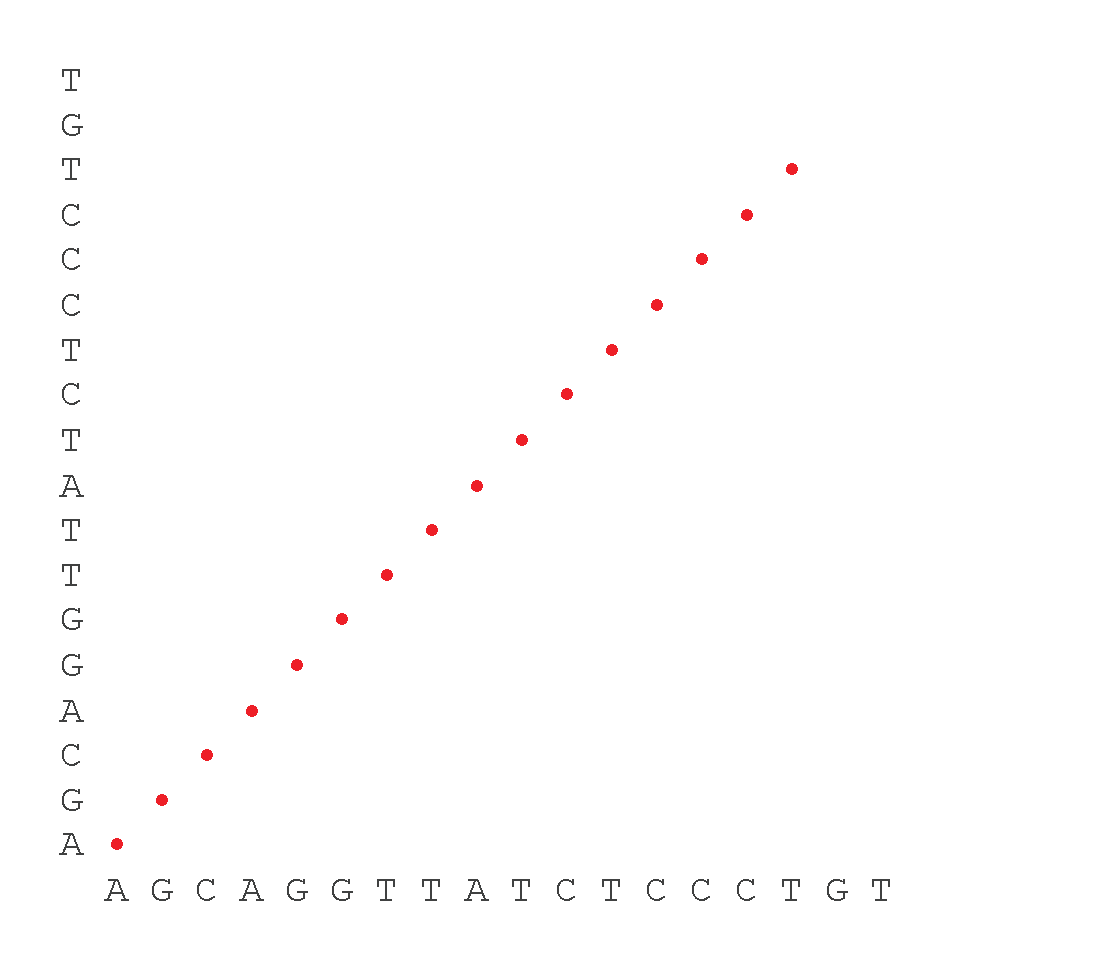
\includegraphics[width = 0.4\textwidth]{images/rearrangements/genomic_dot_plots-1} & 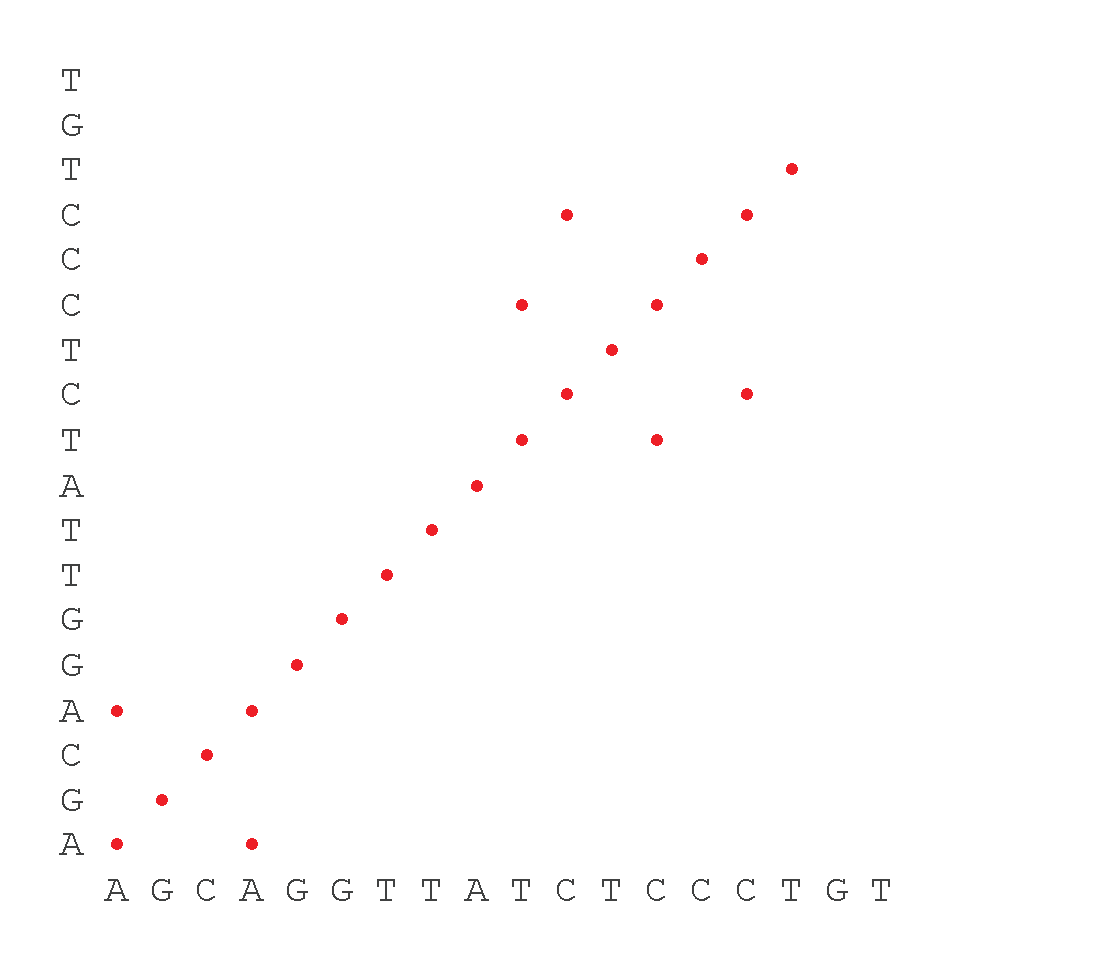
\includegraphics[width = 0.4\textwidth]{images/rearrangements/genomic_dot_plots-2}\\[3ex]
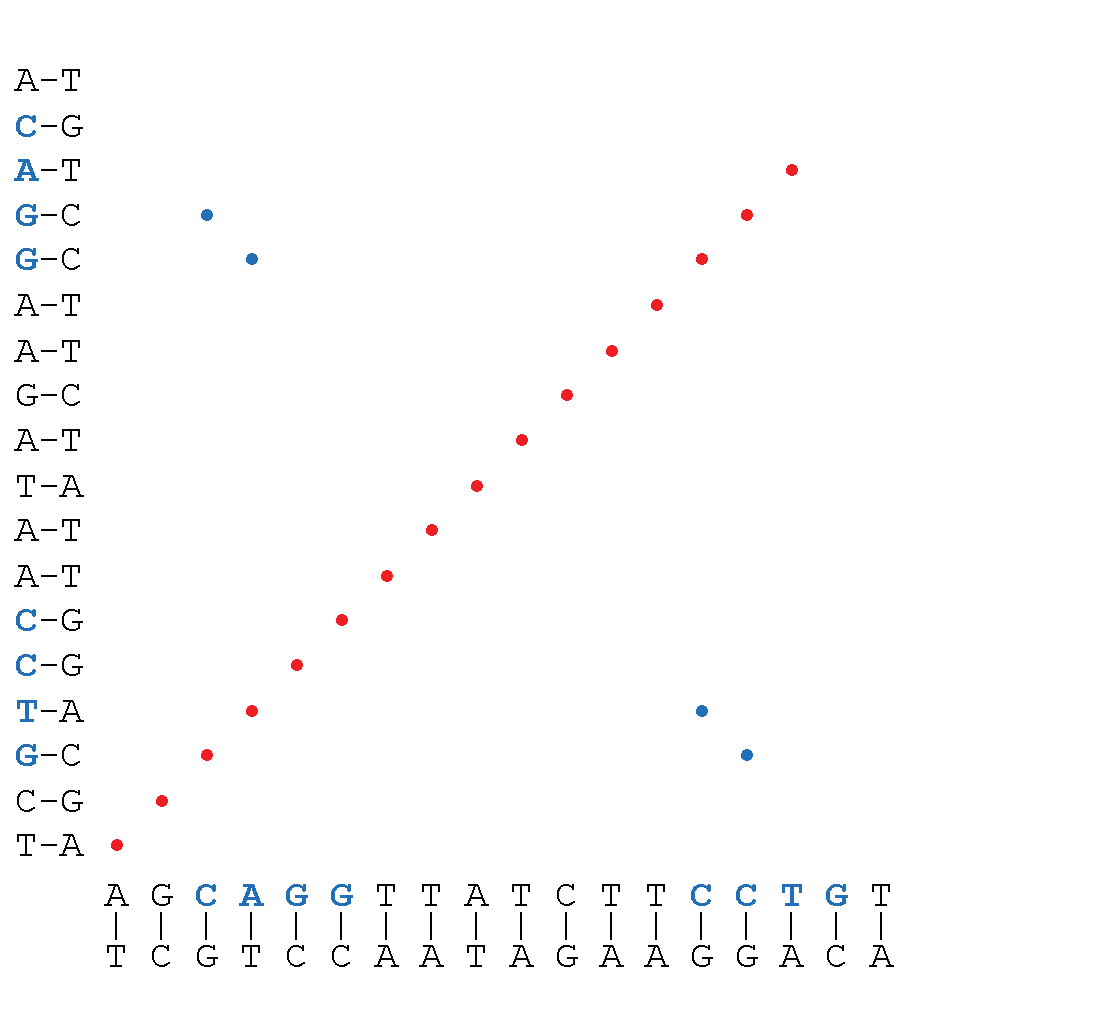
\includegraphics[width = 0.4\textwidth]{images/rearrangements/genomic_dot_plots-3} & 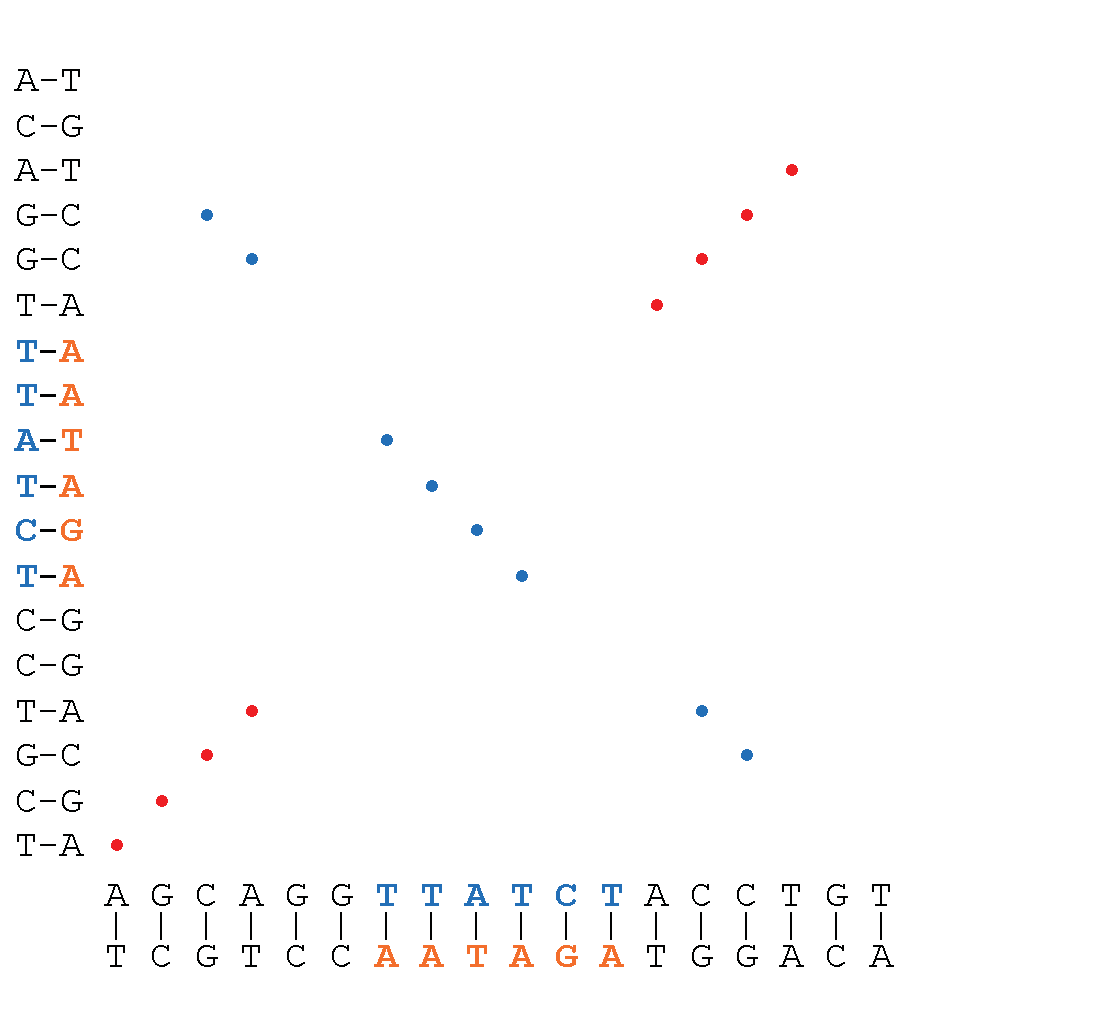
\includegraphics[width = 0.4\textwidth]{images/rearrangements/genomic_dot_plots-4}
\end{tabular}
\caption{A visualization of repeated $k$-mers within the string \textnucl{AGCAGGTTATCTCCCTGT} for $k=3$ (top left) and $k=2$ (top right). (Bottom left) We add blue points to the plot shown in in the upper left corner to indicate reverse complementary $k$-mers.  For example, \textnucl{CCT} and \textnucl{AGG} are reverse complementary 3-mers in \textnucl{AGCAGGTTATCTTCCTGT}. (Bottom right): Genomic dot-plot showing shared 3-mers between \textnucl{\black{AGCAGG}\Blue{TTATCT}\black{CCCTGT}} and \textnucl{\black{AGCAGG}\Orange{AGATAA}\black{CCCTGT}}.  The latter sequence resulted from the former sequence by a reversal of the segment \textnucl{\Blue{TTATCT}}. Each point $(x, y)$ corresponds to a $k$-mer shared by the two genomes.  Red points indicate identical shared $k$-mers, whereas blue points indicate reverse complementary $k$-mers. Note that the dot-plot has four ``noisy'' blue points in the diagram: two in the upper left corner, and two in the bottom right corner. You will also notice that red dots can be connected into line segments with slope 1 and blue dots can be connected into line segments with slope -1. The resulting three synteny blocks (\textnucl{\Red{AGCAGG}}, \textnucl{\Blue{TTATCT}}, and \textnucl{\Red{CCCTGT}}) correspond to three diagonals (each formed by four points) in the dot-plot.}
\label{fig:genomic_dot_plots}
\end{figure}

\begin{center}
\mySfFamily
\tabcolsep = 1em
\begin{tabular}{l l l l}
\textnucl{\phantom{xxxx}}0 & 0 \textnucl{\phantom{xxxx}} & \textnucl{\phantom{xxxx}4} & \textnucl{\phantom{xxxxxx}}6\\[-0.25ex]
\textnucl{\phantom{xxxx}\Red{AAA}CTCATC} & \textnucl{\Blue{AAA}CTCATC} & \textnucl{AAAC\Red{TCA}TC\phantom{xx}} & \textnucl{AAACTC\Red{ATC}}\\
\textnucl{TTTC\Red{AAA}TC\phantom{xxxx}} & \textnucl{\Blue{TTT}CAAATC} & \textnucl{\phantom{xx}TT\Red{TCA}AATC} & \textnucl{TTTCAA\Red{ATC}}\\
\textnucl{\phantom{xxxx}}4 & 0 & \textnucl{\phantom{xxxx}}2 & \textnucl{\phantom{xxxxxx}}6
\end{tabular}
\end{center}

\noindent We can further generalize the genomic dot plot to analyze the shared $k$-mer content of two genomes.  We color the point $(x,y)$ red if the two genomes share a $k$-mer at respective positions $x$ and $y$; we color $(x, y)$ blue if the two genomes have reverse complementary $k$-mers at these starting positions.  See \autoref{fig:genomic_dot_plots} (bottom right).\\

\begin{exercise}[
Find all shared 2-mers of \textnucl{AAACTCATC} and \textnucl{TTTCAAATC}.
]\end{exercise}

\begin{problem}[Shared \textit{k}-mers Problem]{Given two strings, find all their shared \textit{k}-mers.}{An integer $k$ and two strings.}{All $k$-mers shared by these strings, in the form of ordered pairs $(x, y)$.}
\protect\computationalproblem[Shared \textit{k}-mers Problem]{-4.89}
\end{problem}

\noindent Since downloading long human and mouse chromosomes is time-consuming, we will instead solve the Shared $k$-mers Problem for the bacteria \textit{E. coli} and \textit{S. enterica}, which we have already encountered in previous chapters.\\

\begin{exercise}[Answer the following questions regarding counting shared $k$-mers.
\begin{enumerate}
\vspace{-1ex}
\item Compute the expected number of 30-mers shared by two random strings, each a billion nucleotides long.
\vspace{-1ex}
\item How many shared 30-mers do the \textit{E. coli} and \textit{S. enterica} genomes have?
\end{enumerate}
\vspace{-1ex}
]\end{exercise}

\noindent In previous chapters, we have worked with the genomes for the bacteria \textit{E. coli} and \textit{S. enterica}, each of which is about 5 million nucleotides long.  It can be shown that the expected number of shared 30-mers between two random 5 million nucleotide-long sequences is approximately $\left. 2 \cdot (5 \cdot 10^6)^2 \middle/ 4^{30}\right. \approx 1/20,000$.

Yet solving the Shared $k$-mers Problem for \textit{E. coli} and \textit{S. enterica} yields over 200,000 pairs $(x,y)$ corresponding to shared 30-mers. The surprisingly large number of shared 30-mers indicates that \textit{E. coli} and \textit{S. enterica} are close relatives that have retained many similar genes inherited from their common ancestor. However, these genes may be arranged in a different order in the two species: how can we infer synteny blocks from these genomes' shared $k$-mers? The genomic dot-plot plot for \textit{E. coli} and \textit{S. enterica} is shown in \autoref{fig:e-coli_dot-plot}.\par

\begin{figure}[h]
\mySfFamily
\centering
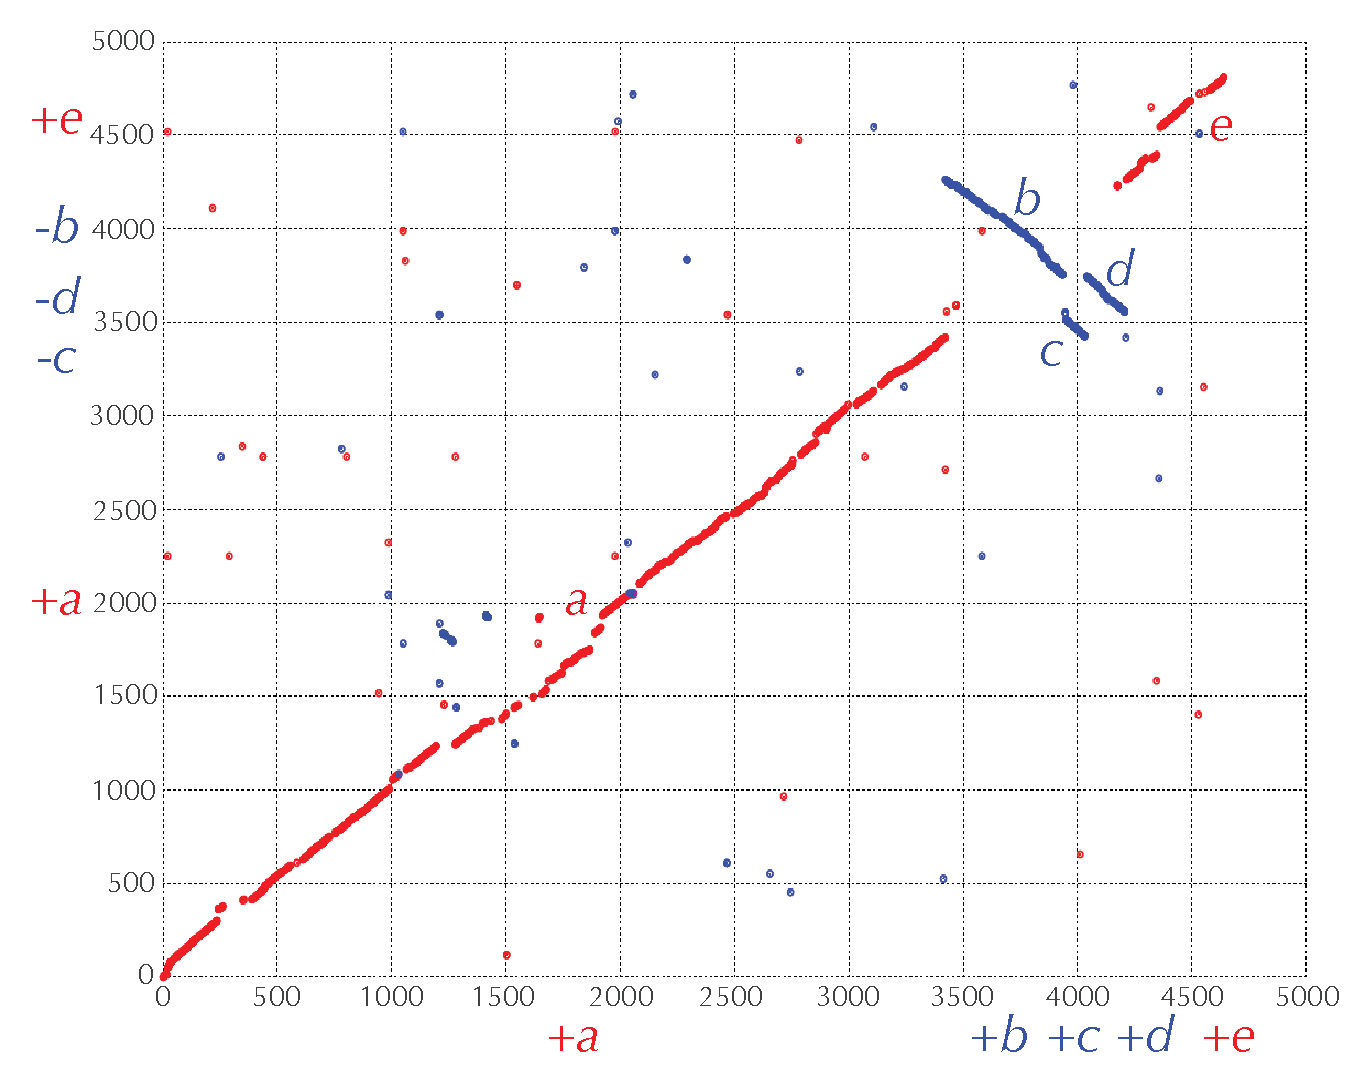
\includegraphics[width = 0.856\textwidth]{images/rearrangements/e-coli_dot-plot}
\caption{Genomic dot-plot of \textit{E. coli} (horizontal axis) and \textit{S. enterica} (vertical axis) for $k = 30$. Each point $(x, y)$ corresponds to a $k$-mer shared by the two genomes.  Red points indicate identical shared $k$-mers, whereas blue points indicate reverse complementary $k$-mers.  Each axis is measured in kilobases (thousands of base pairs).}
\label{fig:e-coli_dot-plot}
\end{figure}

\begin{qbox}[
Can you see the synteny blocks in the genomic dot-plot in \autoref{fig:e-coli_dot-plot}?
]\end{qbox}

\phantomsection
\subsection{From shared \emph{k}-mers to synteny blocks}
\label{subsec:from_shared_k-mers_to_synteny_blocks}

The genomic dot-plot in \autoref{fig:e-coli_dot-plot} indicates five regions of similarity in the form of points that clump together into approximately diagonal segments.  These segments are labeled by \red{\textit{a}}, \blue{\textit{b}}, \blue{\textit{c}}, \blue{\textit{d}}, and \red{\textit{e}} according to the order in which they appear in the \textit{E. coli} genome; we ignore smaller diagonals such as the short blue diagonal starting around position 1.3 million in \textit{E. coli} and around position 1.9 million in \textit{S. enterica}. For example, while \red{\textit{a}} corresponds to a long diagonal segment of slope 1 that covers approximately the first 3.5 million positions in both genomes, \blue{\textit{b}} corresponds to a shorter diagonal segment of slope -1 that starts shortly before position 3.5 million in \textit{E. coli} and shortly after position 4 million in \textit{S. enterica}. Although \blue{\textit{b}} appears small in \autoref{fig:e-coli_dot-plot}, don't be fooled by the scale of the figure; \blue{\textit{b}} is over 100,000 nucleotides long and contains nearly 100 genes.

The segments \red{\textit{a}}, \blue{\textit{b}}, \blue{\textit{c}}, \blue{\textit{d}}, and \red{\textit{e}} give us the synteny blocks that we have been looking for. If we project these blocks onto the $x$- and $y$-axes, then the ordering of blocks on each axis corresponds to the ordering of synteny blocks in the respective bacterium.  The ordering of synteny blocks in \textit{E. coli} (plotted on the $x$-axis) is $(\red{+a}$ $\blue{+b}$ $\blue{+c}$ $\blue{+d}$ $\red{+e})$, and the ordering in \textit{S. enterica} (y-axis) is $(\red{+a}$ $\blue{-c}$ $\blue{-d}$ $\blue{-b}$ $\red{+e})$.  Note that the blue letters in \textit{S. enterica} are assigned a negative sign because these blocks were constructed from reverse complementary $k$-mers. \autoref{fig:e-coli_dot-plot} also illustrates what the directions of blocks are --- they respectively correspond to diagonals in the dot-plot with slope 1 (blocks with a ``+'' sign) and  slope -1 (blocks with a ``-'' sign).

We have therefore represented two bacterial genomes using just five synteny blocks.  Of course, this simplification required us to throw out some noisy points in the genome plot, corresponding to tiny regions of similarity that did not surpass a threshold length in order to be considered synteny blocks.

We are now ready to construct the 11 human-mouse synteny blocks originally presented in \autoref{fig:mouse_and_human_synteny_blocks} (page \pageref{fig:mouse_and_human_synteny_blocks}), but since the human and mouse X chromosomes are rather long, we will instead provide you with all positions $(x,y)$ where they share significant similarities. \autoref{fig:synteny_blocks} (top left) presents the resulting genomic dot-plot for the human and mouse X chromosomes, where each dot represents a long similar region rather than a shared $k$-mer. Our eyes immediately find 11 diagonals in this plot corresponding to the human-mouse X chromosome synteny blocks --- problem solved! We state this problem as the Finding Synteny Blocks Problem.\\

\begin{figure}[p]
\mySfFamily
\centering
\begin{tabular}{c @{\hskip 2em} c}
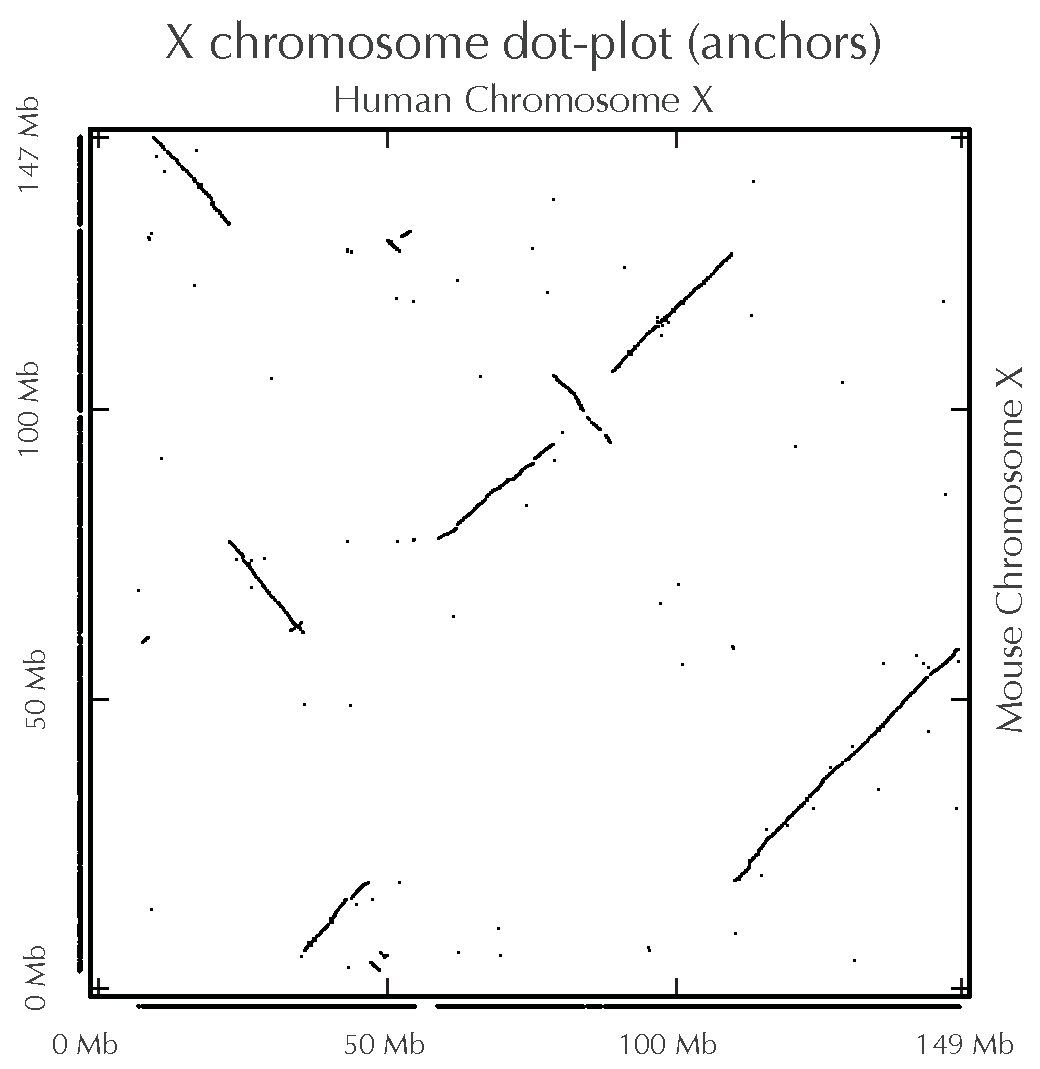
\includegraphics[width = 0.43\textwidth]{images/rearrangements/synteny_blocks-1} & 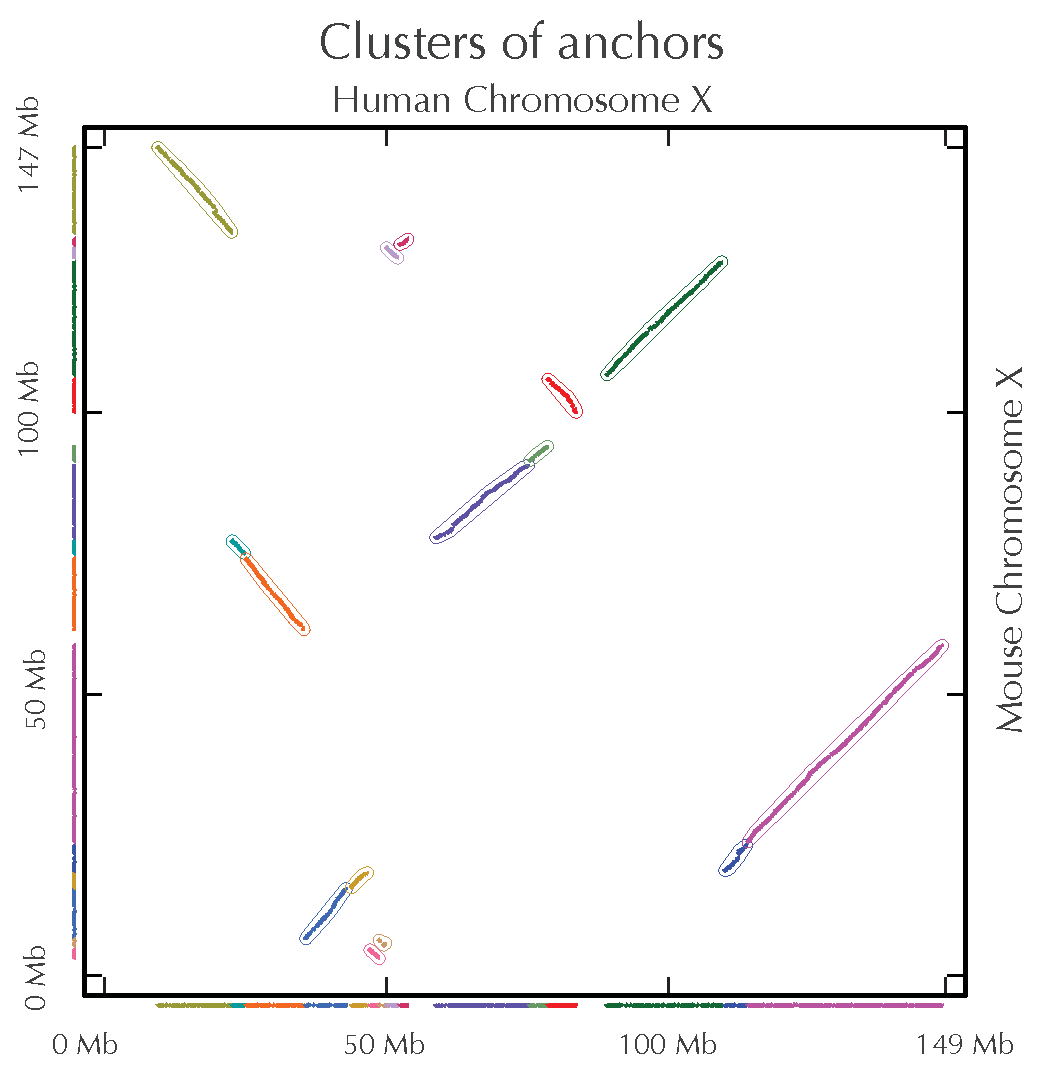
\includegraphics[width = 0.43\textwidth]{images/rearrangements/synteny_blocks-2}\\[3ex]
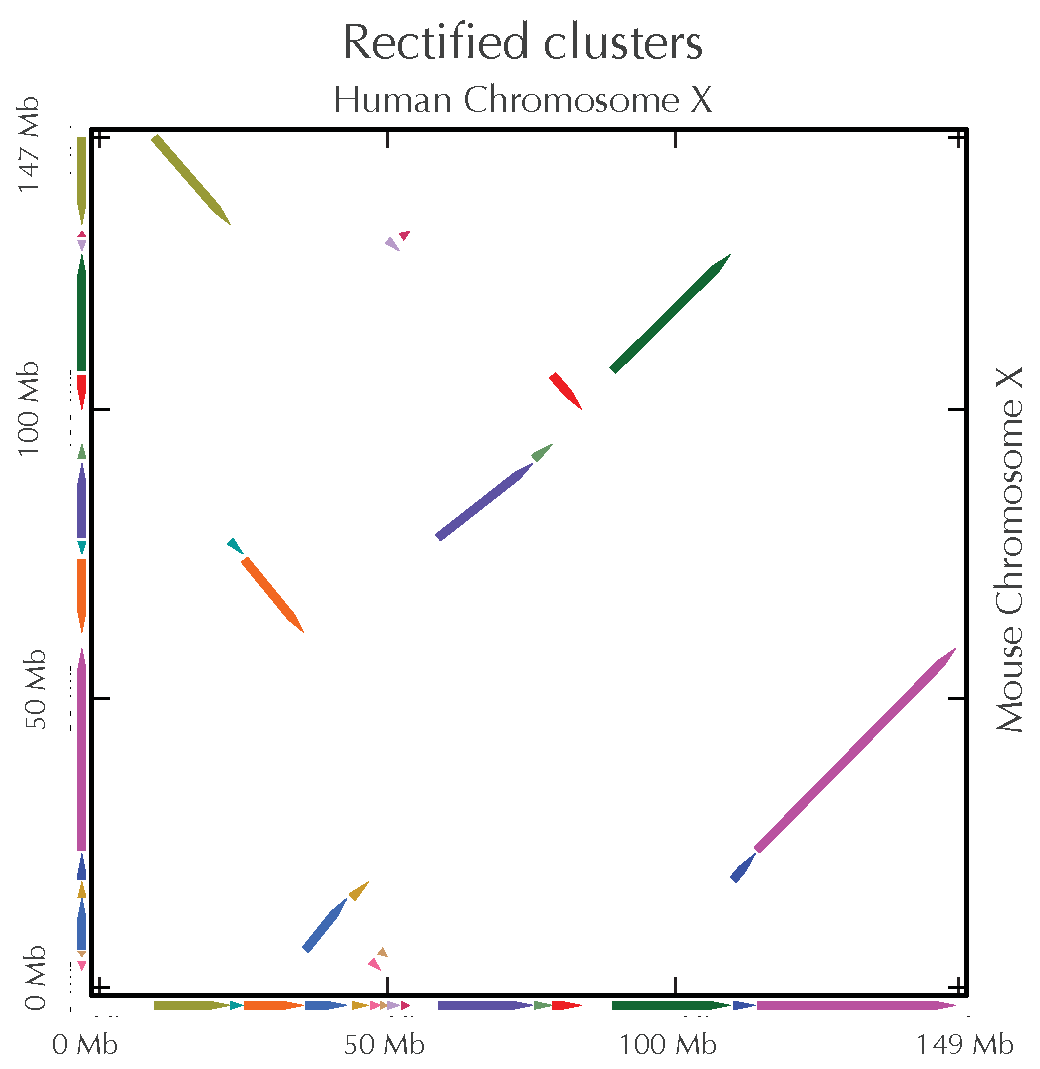
\includegraphics[width = 0.43\textwidth]{images/rearrangements/synteny_blocks-3} & 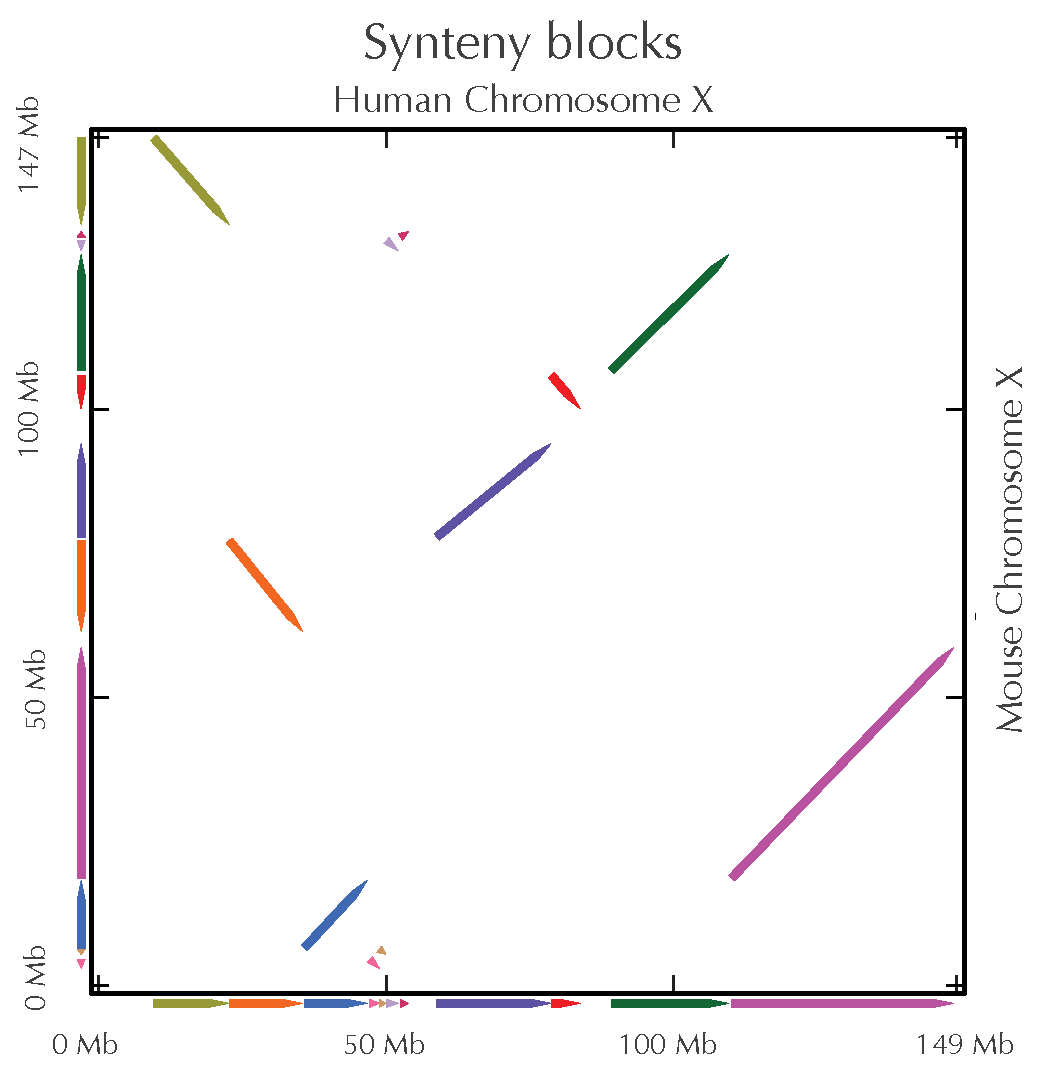
\includegraphics[width = 0.43\textwidth]{images/rearrangements/synteny_blocks-4}\\[3ex]
\end{tabular}
\caption{From local similarities to synteny blocks. (Top left) The genomic dot-plot for the human and mouse X chromosomes, representing all positions $(x,y)$ where they share significant similarities.  In contrast with \autoref{fig:e-coli_dot-plot}, we do not distinguish between red and blue dots. (Top right) Clusters (connected components) of points in the genomic dot-plot are formed by constructing the synteny graph.  (Bottom left) Rectified clusters from the synteny graph transform each cluster into an exact diagonal of slope $\pm 1$. (Bottom right) Aggregated synteny blocks.  Projection of the synteny blocks to the $x$-and $y$-axes results in the arrangements of synteny blocks in the respective human and mouse genomes $(+1$ $+2$ $+3$ $+4$ $+5$ $+6$ $+7$ $+8$ $+9$ $+10$ $+11)$ and  $(+1$ $-7$ $+6$  $-10$  $+9$  $-8$  $+2$ $-11$ $-3$ $+5$ $+4)$.}
\label{fig:synteny_blocks}
\end{figure}

\begin{problem}[Finding Synteny Blocks Problem]{Find diagonals in the genomic dot-plot.}{A set of points \textvar{DotPlot} in the plane.}{A set of diagonals in \textvar{DotPlot} representing synteny blocks.}
\end{problem}

\noindent Unfortunately, it remains unclear how to write a program to do what our eyes found to be so easy; we hope you have already noticed that the Finding Synteny Blocks Problem is not a well-formulated computational problem. As we have mentioned, the diagonals in \autoref{fig:synteny_blocks} (top left) are not perfect. Moreover, there are many gaps within diagonals that cannot be seen by the human eye but will become apparent if we zoom into the genome plot. It is thus absolutely unclear what method the human brain is using to transform the dots into the 11 diagonals in the genomic dot-plot.\\

\begin{qbox}[
How can we translate the brain's tendency to construct the diagonals that you see in \autoref{fig:synteny_blocks} (top left) into an algorithm that a computer can understand?
]\end{qbox}

\vspace{-0.5\baselineskip}

\phantomsection
\subsection{Synteny blocks as connected components in graphs}
\label{subsec:synteny_blocks_as_connected_components_in_graphs}

The reason why you can easily see the synteny blocks in a genomic dot-plot is that your brain is good at \textdef{clustering} nearby points in an image.  To mimic this process with a computer, we therefore need a precise notion of clustering. Given a set of points \textvar{DotPlot} in the plane as well as a parameter \textit{maxDistance}, we will construct the (undirected) \textdef{synteny graph} $\textfunc{SyntenyGraph}(\textvar{DotPlot}, \textvar{maxDistance})$ by connecting two points in \textvar{DotPlot} with an edge if the distance between them does not exceed \textvar{maxDistance}.

Every graph can be divided into disjoint connected subgraphs called \textdef{connected components}.  The connected components in $\textfunc{SyntenyGraph}(\textvar{DotPlot}, \textvar{maxDistance})$ represent candidate synteny blocks between the two genomes (\autoref{fig:synteny_graph}).  When we construct the synteny graph for the human and mouse X chromosomes, we find a huge number of small connected components (the exact number depends on our choice of the \textvar{maxDistance} parameter). However, we will ignore these small connected components, since they may represent spurious similarities. We thus introduce a parameter called \textvar{minSize} representing the minimum number of points in a connected component that we will consider as forming a synteny block.  Our goal is to return all connected components having at least \textvar{minSize} nodes.\\

\begin{figure}[h]
\mySfFamily
\centering
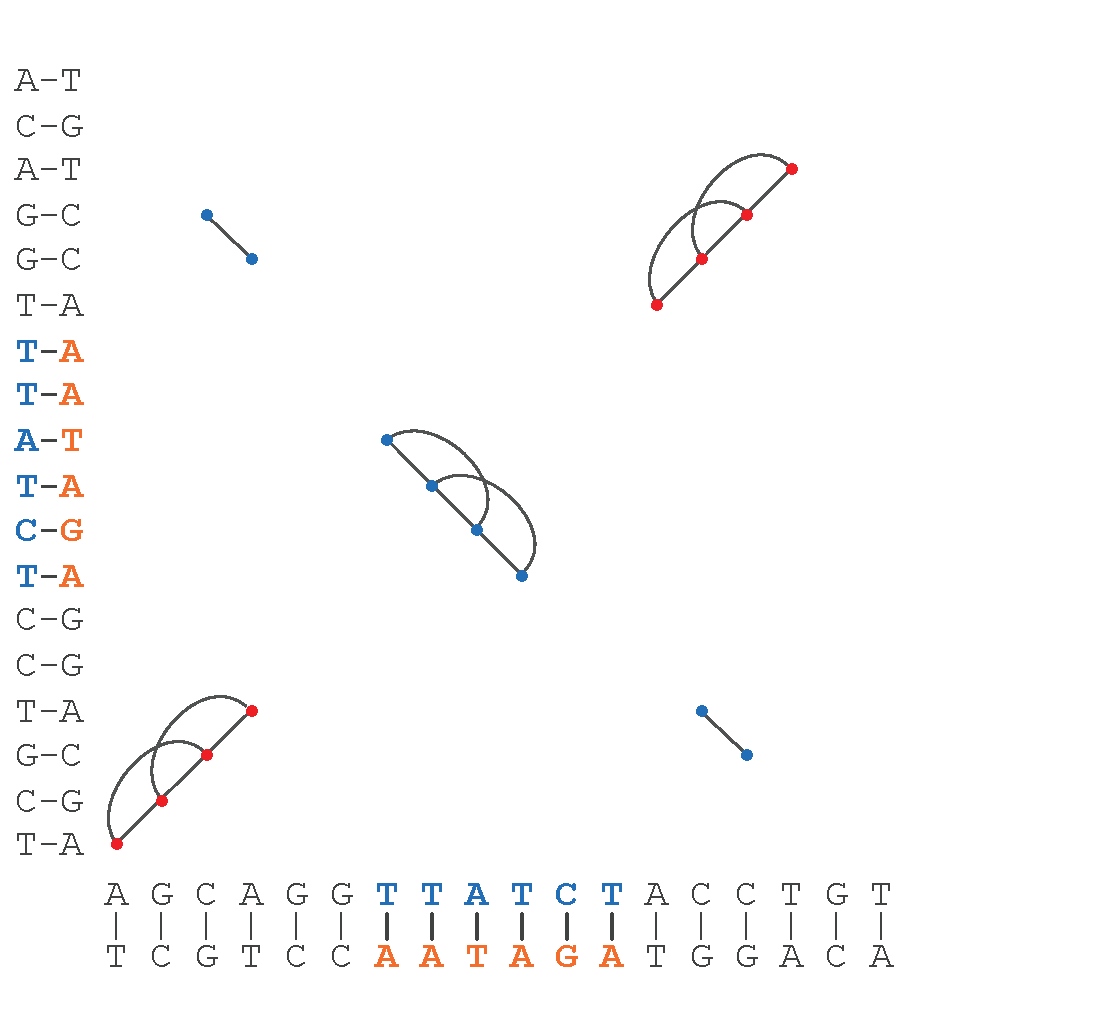
\includegraphics[width = 0.6\textwidth]{images/rearrangements/synteny_graph}
\caption{The graph $\textfunc{SyntenyGraph}(\textvar{DotPlot}, 4)$ constructed from the genomic dot-plot of \textnucl{\black{AGCAGG}\Blue{TTATCT}\black{CCCTGT}} and \textnucl{\black{AGCAGG}\Orange{AGATAA}\black{CCCTGT}}  for $k = 3$.  Note that the three synteny blocks (all of which have four nodes) correspond to diagonals in the genomic dot-plot.  We ignore the two smaller, noisy synteny blocks.}
\label{fig:synteny_graph}
\end{figure}

\begin{elaboration}
\begin{algorithmic}
\leftskip = \algindent %Needed to match the indentation of the text.
\Algorithm{SyntenyBlocks}{\textvar{DotPlot}, \textvar{maxDistance}, \textvar{minSize}}
	\State construct $\textfunc{SyntenyGraph}(\textvar{DotPlot}, \textvar{maxDistance})$
	\State find the connected components in $\textfunc{SyntenyGraph}(\textvar{DotPlot}, \textvar{maxDistance})$
	\State \output connected components of at least \textvar{minSize} nodes as candidate\\ \hspace{4.7em}synteny blocks
\EndAlgorithm
\end{algorithmic}
\end{elaboration}
%\protect\computationalproblem[e]{Find Synteny Blocks}{-27.5}

\fudgespace

\noindent As \autoref{fig:synteny_blocks} (top right) illustrates, \textalg{SyntenyBlocks} has a tendency to partition a single diagonal (as perceived by the human eye) into multiple diagonals due to gaps that exceed the parameter \textvar{maxDistance}. However, this partitioning is not a problem, since the broken diagonals can be combined later into a single (aggregated) synteny block. \par

\vspace{\baselineskip}

\begin{qbox}[
We have defined synteny blocks as large connected components in $\textfunc{SyntenyGraph}(\textvar{DotPlot}, \textvar{maxDistance})$ but have not described how to determine where these synteny blocks are located in the original genomes. Using \autoref{fig:synteny_blocks} as a hint, design an algorithm for finding this information.
]\end{qbox}

\noindent You should now be ready to solve the challenge problem and discover that the choice of parameters is one of the dark secrets of bioinformatics research.\\

\begin{finalchallenge}[Analyze Rearrangements Between X Chromosomes]{
Construct the synteny blocks for the human and mouse X chromosomes and compute the 2-break distance between the circularized human and mouse X chromosomes using the synteny blocks that you constructed. How does this distance change depending on the parameters \textvar{maxDistance} and \textvar{minSize}?
}\end{finalchallenge}

\phantomsection
\FloatBarrier
\section{Open Problem: Can Rearrangements Shed Light on Bacterial Evolution?}
\label{sec:rearrangements_open_problem}

Although there exist efficient algorithms for analyzing \emph{pairwise} genome rearrangements, constructing rearrangement scenarios for \emph{multiple} genomes remains an open problem. For example, we now know how to find a most parsimonious rearrangement scenario transforming the mouse X chromosome into the human X chromosome. However, the problem of finding a most parsimonious rearrangement scenario for the human, mouse and rat X chromosomes (let alone for their entire genomes) is a more difficult problem. The difficulties further amplify when we attempt to reconstruct a rearrangement history for dozens of mammalian genomes. To address this challenge, we start from the simpler (but still unsolved) case of bacterial genomes.

Let \textvar{Tree} be a tree (i.e., a connected acyclic undirected graph) with nodes labeled by some genomes. In the case of bacterial genomes, we assume that every node (genome) is labeled by a circular permutation on $n$ elements. Given an edge $e$ connecting nodes $v$ and $w$ in \textvar{Tree}, we define $\textfunc{Distance}(v, w)$ as the 2-break distance between genomes $v$ and $w$.  The \textdef{tree distance} $\textfunc{Distance}(\textvar{Tree})$ is the sum 

\begin{center}
$\sum\limits_{\text{all edges }(v, w)\text{ in \textvar{Tree}}}{\textfunc{Distance}(v, w)}$.
\end{center}

Given a set of genomes $P_1, \ldots ,P_n$ and an evolutionary tree \textvar{Tree} with $n$ leaves labeled by $P_1, \ldots ,P_n$, the Ancestral Genome Reconstruction Problem attempts to reconstruct  genomes at the internal nodes of the tree such that $\textfunc{Distance}(\textvar{Tree})$ is minimized across all possible reconstructions of genomes at internal nodes.\\

\begin{problem}[Ancestral Genome Reconstruction Problem]{Given a tree with leaves labeled by genomes, reconstruct ancestral genomes that minimize the tree distance.}{A tree \textvar{Tree} with each leaf labeled by a genome.}{Genomes \textvar{AncestralGenomes} assigned to the internal nodes of \textvar{Tree} such that $\textfunc{Distance}(\textvar{Tree})$ is minimized across all possible choices of \textvar{AncestralGenomes}.}
\end{problem}

\noindent In the case when \textvar{Tree} is not given, we need to infer it from the genomes.\\

\begin{problem}[Multiple Genome Rearrangement Problem]{Given a set of genomes, reconstruct a tree with leaves labeled by these genomes and minimum tree distance.}{A set of genomes.}{A tree \textvar{Tree} with leaves labeled by these genomes and internal nodes labeled by (unknown) genomes \textvar{AncestralGenomes} such that $\textfunc{Distance}(\textvar{Tree})$ is minimal among all possible choices of \textvar{Tree} and \textvar{AncestralGenomes}.}
\end{problem}

\noindent While many algorithms have been proposed for the Multiple Genome Rearrangement Problem, they have mainly been applied to analyze mammalian evolution (see \cite{ma_2008} and \cite{alekseyev_pevzner_2009} for some examples).  However, there have been hardly any applications of the Multiple Genome Rearrangement Problem for analyzing bacterial evolution. The fact that bacterial genomes are approximately 1000 times smaller than mammalian genomes does not make this problem 1000 times easier. In fact, there are unique challenges and opportunities in bacterial evolutionary research.

Consider 100 genomes from three closely related bacterial genera, \textit{Salmonella}, \textit{Shigella}, and \textit{Escherichia}, whose various species are responsible for dysentery, typhoid fever, and a variety of foodborne illnesses.  After you construct synteny blocks shared by all these genomes, you will see that there are relatively few (usually fewer than 10) rearrangements between every pair of genomes. However, solving the Multiple Genome Rearrangement Problem even in the case of closely related genomes presents a formidable challenge, and nobody has been able to construct a rearrangement scenario for more than a couple dozen --- let alone 100! --- species yet.

After you solve this puzzle, you will be able to address the question of whether there are fragile regions in bacterial genomes. Answering this question for a pair of bacterial genomes, like we did for the human and mouse genomes, may not be possible because there are typically fewer than 10 rearrangements between them. But answering this question for 100 bacterial genomes may be possible if we witness the same breakage occurring independently on many branches of the evolutionary tree. However, you will need to develop algorithms to analyze fragile regions in multiple (rather than pairwise) genomes.

After you construct the evolutionary tree, you will also be in a position to analyze the question of what triggers rearrangements. While many authors have discussed the causes of fragility, this question remains open, with no shortage of hypotheses. \cite{zhao_bourque_2009} demonstrated that many rearrangements are flanked by \textdef{matching duplications}, a pair of long similar regions located within a pair of breakpoint regions corresponding to a rearrangement event. However, they limited their study to mammalian evolution, and it remains unclear what triggers rearrangements in bacteria; can you answer this question?\\

\phantomsection
\FloatBarrier
\section{Detours}
\label{sec:detours_rearrangements}

\phantomsection
\begin{detour}[Why is the gene content of mammalian X chromosomes so conserved?]{why_is_the_gene_content_of_mammalian_x_chromosomes_so_conserved}

While mammalian X chromosomes are enriched in genes related to sexual reproduction, most of the approximately 1000 genes on the X chromosome have nothing to do with gender. Ideally, they should be expressed (i.e., transcribed and eventually translated) in roughly the same quantities in females and males.  But since females have two X chromosomes and males have only one, it would seem that all the genes on the X chromosome should have twice the expression level in females.  This imbalance would lead to a problem in the complex cellular system of checks and balances underlying gene expression.

The need to balance gene expression in males and females led to the evolution of special mechanisms of \textdef{dosage compensation}, or the inactivation of one X chromosome in females to equalize gene expression between the sexes. Because of dosage compensation, the gene content of the X chromosome is highly conserved between mammalian species because if a gene jumps off the X chromosome, then its expression may double, thus creating a genetic imbalance.
\end{detour}

\phantomsection
\begin{detour}[Discovery of genome rearrangements]{discovery_of_genome_rearrangements}
\textdef{Genetic maps}, which show the positions of genes along chromosomes, were used by Thomas Hunt Morgan's lab at Columbia as early as 1913.  An amazing thing happened in 1921 when Morgan's student Alfred Sturtevant created genetic maps for two different species of \textit{Drosophila}. It was clear just by looking at the maps that an entire genomic interval had been inverted in one species as compared to another! The only reasonable explanation was that a reversal had flipped this chromosomal interval around. Sturtevant posited that this had happened when the chromosome became tangled on itself and formed a loop.

Another breakthrough occurred with the discovery that the salivary glands of \textit{Drosophila} contain \textdef{polytene cells}.  In normal cellular division, each daughter cell receives one copy of the genome.  However, in the nuclei of polytene cells, DNA replication occurs repeatedly in the absence of cell division.  The resulting chromosomes then knit themselves together into much larger ``superchromosomes'' called \textdef{polytene chromosomes}.

Polytene chromosomes serve a practical purpose for the fruit fly, which uses the extra DNA to boost the production of gene transcripts, producing lots of sticky saliva. But the human value of polytene chromosomes is perhaps greater.  When Sturtevant and his collaborator, Theodosius Dobzhansky, looked at polytene chromosomes under a microscope, they were able to witness the work of rearrangements  firsthand in tangled mutant chromosomes. In 1938, Sturtevant and Dobzhansky published a milestone paper with an evolutionary tree presenting a rearrangement scenario with 17 reversals for various species of \textit{Drosophila}. Their drawing was the first evolutionary tree in history to be constructed based on molecular data.

%\begin{figure}[h]
%\mySfFamily
%\centering
%\textbf{THIS FIGURE IS DEFINITELY COPYRIGHTED}
%\caption{Evolutionary tree of various \textit{Drosophila} species based on their gene arrangements. Two species connected by an edge in the tree differ by a single reversal.}
%\label{fig:drosophila_phylogeny}
%\end{figure}
\end{detour}

\phantomsection
\begin{detour}[The exponential distribution]{the_exponential_distribution}
A \textdef{Bernoulli trial} is a random experiment with two possible outcomes, ``success'' (having probability $p$) and ``failure'' (having probability $1-p$). The \textdef{geometric distribution} is the probability distribution underlying the random variable $X$ representing the number of Bernoulli trials needed to obtain the first success:

\begin{center}
$\mathrm{Pr}(X = k) = (1-p)^{k-1}p$.
\end{center}

A \textdef{Poisson process} is a continuous-time stochastic process counting the number of events in a given time interval, if we assume that the events occur independently at a constant rate. For example, the Poisson process offers a good model of time points for passengers arriving to a large train station.  If we assume that the number of passengers arriving during a very small time interval $\epsilon$ is $\lambda \cdot \epsilon$ (where $\lambda$ is a constant), then we are interested in the probability $F(X)$ that nobody will arrive to the station during a time interval $X$. The \textdef{exponential distribution} describes the time between events in a Poisson process.\\

\begin{qbox}[
Do you see any similarities between the Poisson process and the Bernoulli trials or between the exponential and geometric distributions? 
]\end{qbox}

\noindent The exponential distribution is merely the continuous analogue of the geometric distribution. More precisely, the Poisson process is characterized by a \textdef{rate parameter} $\lambda$, such that the number of events $k$ in the time interval $[X, X+\epsilon]$ follows the \textdef{Poisson probability distribution}:

\begin{center}
$\left. e^{-\lambda \cdot \epsilon}(\lambda \cdot \epsilon)^k \middle/ k!\right.$
\end{center}

\noindent The \textdef{probability density function} of the exponential distribution is  $\lambda e^{-\lambda \cdot X}$ (compare with the geometric distribution shown in \autoref{fig:probability_density_functions}).\\

\begin{figure}[h]
\centering
\begin{tabular}{c @{\hskip3em} c}
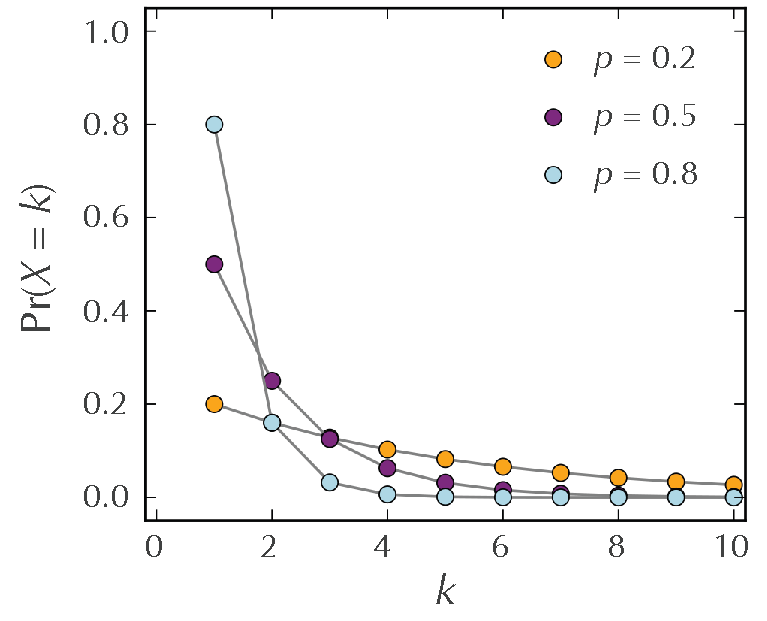
\includegraphics[width = 0.4\textwidth, valign = b]{images/rearrangements/geometric_distribution} & 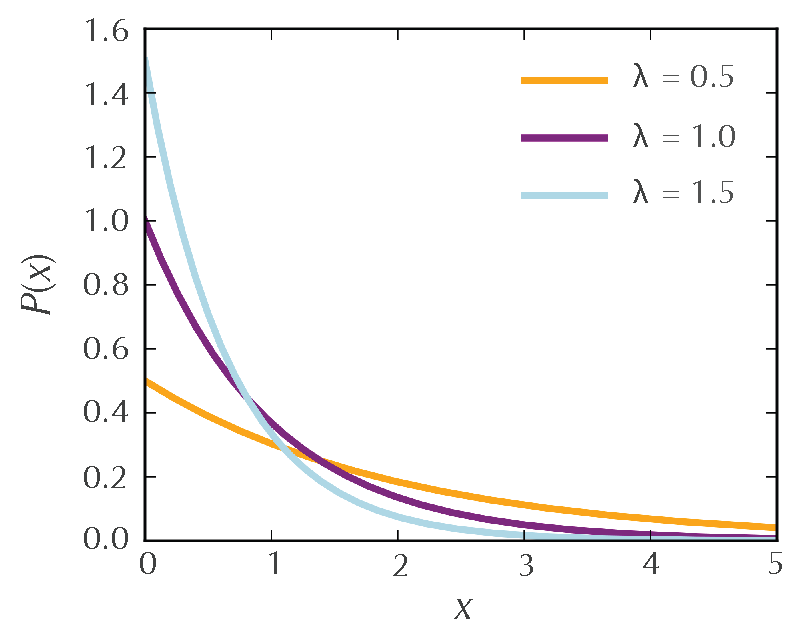
\includegraphics[width = 0.42\textwidth, valign = b]{images/rearrangements/exponential_distribution}\\
\end{tabular}
\caption{The probability density functions of the geometric (left) and exponential (right) distributions, each provided for three different parameter values.  Courtesy Skbkekas (Wikipedia user).}
\label{fig:probability_density_functions}
\end{figure}

\end{detour}

%\phantomsection
%\begin{detour}[Occam's Razor]{occams_razor}
%William of Ockham was an influential philosopher in the 14th Century. The principle of Occam's razor states that one should proceed to simpler theories until simplicity can be traded for greater explanatory power. Though the principle is attributed to Occam, Ptolemy (c. AD 90 -- c. AD 168) stated, ``We consider it a good principle to explain the phenomena by the simplest hypothesis possible.''  Thomas Aquinas (1225-1274) added that ``it is superfluous to suppose that what can be accounted for by a few principles has been produced by many''.  After Occam, Isaac Newton (1642-1727) stated, ``We are to admit no more causes of natural things than such as are both true and sufficient to explain their appearances.'' Francis Crick, on the other hand, commented on limitations of Occam's razor in biology: ``While Occam's razor is a useful tool in the physical sciences, it can be a very dangerous implement in biology. It is thus very rash to use simplicity and elegance as a guide in biological research.''
%\end{detour}

\vspace{-0.5\baselineskip}

\phantomsection
\begin{detour}[Bill Gates and David X. Cohen flip pancakes]{bill_gates_and_david_x_cohen_flip_pancakes}
Before biologists faced genome rearrangement problems, mathematicians posed the \textdef{Pancake Flipping Problem}, arising from the following hypothetical waiter's conundrum.

\begin{quote}
\textit{The chef in our place is sloppy, and when he prepares a stack of pancakes they come out all different sizes. Therefore, when I deliver them to a customer, on the way to a table I rearrange them (so that the smallest winds up on top, and so on, down to the largest at the bottom) by grabbing several from the top and flipping them over, repeating this (varying the number I flip) as many times as necessary. If there are $n$ pancakes, what is the maximum number of flips that I will ever have to use to rearrange them?}
\end{quote}

Formally, a \textdef{prefix reversal} is a reversal that flips a prefix, or initial interval, of a permutation. The \textdef{Pancake Flipping Problem} corresponds to sorting unsigned permutations by prefix reversals.  For example, the series of prefix reversals shown below ignores signs and represents the sorting of an \textdef{unsigned permutation}, $(1 ~ 7 ~ 6 ~ 10 ~ 9 ~ 8 ~ 2 ~ 11 ~ 3 ~ 5 ~ 4)$, into the \textdef{identity unsigned permutation}, $(1 ~ 2 ~ 3 ~ 4 ~ 5 ~ 6 ~ 7 ~ 8 ~ 9 ~ 10 ~ 11)$.  The inverted interval is shown in red, and sorted intervals at the end of the permutation are shown in blue.

\begin{center}
\mySfFamily
\tabcolsep = 0.5em
\begin{tabular}{r @{\hskip0em} c c c c c c c c c c c @{\hskip0em} l}
$($ & \Red{1} & \Red{7} & \Red{6} & \Red{10} & \Red{9} & \Red{8} & \Red{2} & \Red{11} & 3 & 5 & 4 & $)$\\[-0.25ex]
$($ & \Red{11} & \Red{2} & \Red{8} & \Red{9} & \Red{10} & \Red{6} & \Red{7} & \Red{1} & \Red{3} & \Red{5} & \Red{4} & $)$\\[-0.25ex]
$($ & \Red{4} & \Red{5} & \Red{3} & \Red{1} & \Red{7} & \Red{6} & \Red{10} & 9 & 8 & 2 & \Blue{11} & $)$\\[-0.25ex]
$($ & \Red{10} & \Red{6} & \Red{7} & \Red{1} & \Red{3} & \Red{5} & \Red{4} & \Red{9} & \Red{8} & \Red{2} & \Blue{11}& $)$\\[-0.25ex]
$($ & \Red{2} & \Red{8} & \Red{9} & 4 & 5 & 3 & 1 & 7 & 6 & \Blue{10} & \Blue{11} & $)$\\[-0.25ex]
$($ & \Red{9} & \Red{8} & \Red{2} & \Red{4} & \Red{5} & \Red{3} & \Red{1} & \Red{7} & \Red{6} & \Blue{10} & \Blue{11}& $)$\\[-0.25ex]
$($ & \Red{6} & \Red{7} & 1 & 3 & 5 & 4 & 2 & \Blue{8} & \Blue{9} & \Blue{10} & \Blue{11} & $)$\\[-0.25ex]
$($ & \Red{7} & \Red{6} & \Red{1} & \Red{3} & \Red{5} & \Red{4} & \Red{2} & \Blue{8} & \Blue{9} & \Blue{10} & \Blue{11} & $)$\\[-0.25ex]
$($ & \Red{2} & \Red{4} & \Red{5} & 3 & 1 & \Blue{6} & \Blue{7} & \Blue{8} & \Blue{9} & \Blue{10} & \Blue{11} & $)$\\[-0.25ex]
$($ & \Red{5} & \Red{4} & \Red{2} & \Red{3} & \Red{1} & \Blue{6} & \Blue{7} & \Blue{8} & \Blue{9} & \Blue{10} & \Blue{11} & $)$\\[-0.25ex]
$($ & \Red{1} & \Red{3} & 2 & \Blue{4} & \Blue{5} & \Blue{6} & \Blue{7} & \Blue{8} & \Blue{9} & \Blue{10} & \Blue{11} & $)$\\[-0.25ex]
$($ & \Red{3} & \Red{1} & \Red{2} & \Blue{4} & \Blue{5} & \Blue{6} & \Blue{7} & \Blue{8} & \Blue{9} & \Blue{10} & \Blue{11} & $)$\\[-0.25ex]
$($ & \Red{2} & \Red{1} & \Blue{3} & \Blue{4} & \Blue{5} & \Blue{6} & \Blue{7} & \Blue{8} & \Blue{9} & \Blue{10} & \Blue{11} & $)$\\[-0.25ex]
$($ & \Blue{1} & \Blue{2} & \Blue{3} & \Blue{4} & \Blue{5} & \Blue{6} & \Blue{7} & \Blue{8} & \Blue{9} & \Blue{10} & \Blue{11} & $)$\\
\end{tabular}
\end{center}

When we instead desire a minimum series of prefix reversals sorting a \emph{signed} permutation, the problem is called the \textdef{Burnt Pancake Flipping Problem} (each pancake is ``burnt'' on one side, giving it two possible orientations).\\

\begin{qbox}[
Prove that every unsigned permutation of length $n$ can be sorted using at most  $2 \cdot (n-1)$ prefix reversals.  Prove that every signed permutation of length $n$ can be sorted using at most $3 \cdot (n-1) + 1$ prefix reversals. 
]\end{qbox}

\noindent Bill Gates, an undergraduate student at Harvard in the mid-1970s, and Christos Papadimitriou, a professor at Harvard in the mid-1970s, made the first attempt to solve the Pancake Flipping Problem and proved that any permutation of length $n$ can be sorted with at most $5/3 \cdot (n + 1)$ prefix reversals, a result that would not be improved for three decades. David X. Cohen worked on the Burnt Pancake Flipping Problem at Berkeley before he left computer science to become a writer for \textit{The Simpsons} and eventually producer of \textit{Futurama}. Along with Manuel Blum, he demonstrated that the Burnt Pancake Flipping Problem can be solved with at most $2 \cdot (n - 1)$ prefix reversals.

\end{detour}

\phantomsection
\begin{detour}[Similar problems with different fates]{similar_problems_with_different_fates}
In the main text, we defined the breakpoint graph for circular chromosomes, but this structure can easily be extended to linear chromosomes. \autoref{fig:permutation_breakpoint_graph} depicts the human and the mouse X chromosomes as alternating red-black and blue-black paths (1st and 2nd panels). These two paths are superimposed in the 3rd panel to form the breakpoint graph, which has 5 alternating red-blue cycles.\\

\begin{figure}[h]
\mySfFamily
\centering
\begin{tabular}{c}
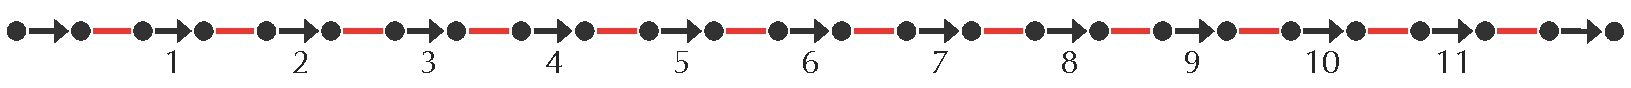
\includegraphics[width = 0.856\textwidth]{images/rearrangements/permutation_breakpoint_graph_1}\\[3ex]
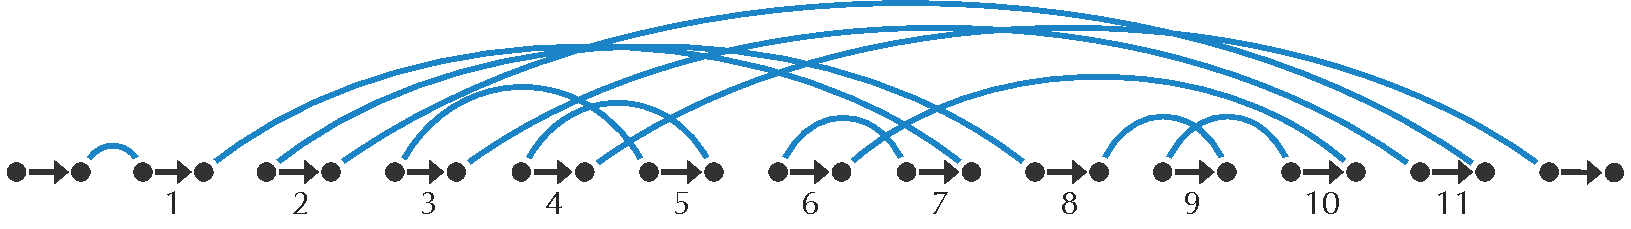
\includegraphics[width = 0.856\textwidth]{images/rearrangements/permutation_breakpoint_graph_2}\\[3ex]
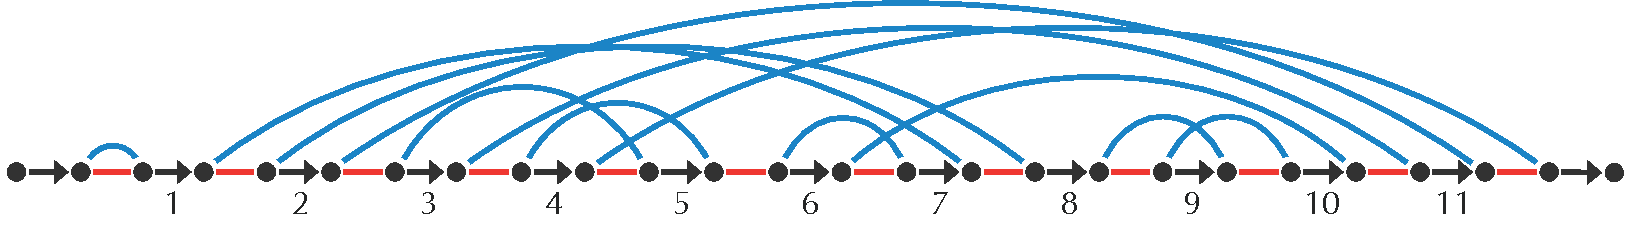
\includegraphics[width = 0.856\textwidth]{images/rearrangements/permutation_breakpoint_graph_3}\\[3ex]
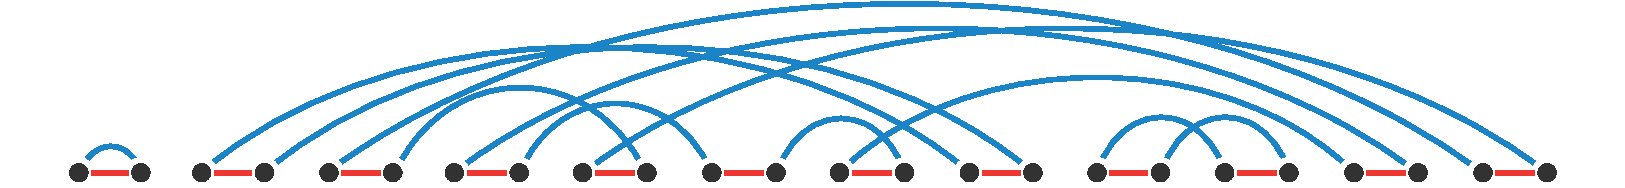
\includegraphics[width = 0.856\textwidth]{images/rearrangements/permutation_breakpoint_graph_4}
\end{tabular}
\caption{(1st panel) An alternating path of red and black edges representing the human X chromosome $(+1$ $+2$ $+3$ $+4$ $+5$ $+6$ $+7$ $+8$ $+9$ $+10$ $+11)$.   (2nd panel) An alternating path of blue and black edges representing the mouse X chromosome $(+1$ $-7$ $+6$ $-10$ $+9$ $-8$ $+2$ $-11$ $-3$ $+5$ $+4)$. (3rd panel) The breakpoint graph of the mouse and human X chromosomes is obtained by superimposing red-black and blue-black paths from the first two panels. (4th panel) To highlight the five alternating red-blue cycles in the breakpoint graph, black edges are removed.}
\label{fig:permutation_breakpoint_graph}
\end{figure}

\begin{qbox}[
Prove the following analogue of the Cycle Theorem for permutations: Given permutations $P$ and $Q$, any reversal applied to $P$ can increase $\textfunc{Cycles}(P, Q)$ by at most 1.
]\end{qbox}

\noindent While the number of trivial cycles is equal to $\textfunc{Blocks}(Q, Q)$  in the identity breakpoint graph of a circular permutation,  the trivial breakpoint graph of a linear permutation has $\textfunc{Blocks}(Q, Q) + 1$ trivial cycles.  Since the Cycle Theorem holds for linear permutations, perhaps the reversal distance $d_{\text{rev}}(P, Q)$ is equal to $\textfunc{Blocks}(P, Q) + 1 - \textfunc{Cycles}(P, Q)$ for linear chromosomes?  After all, for the human and mouse X chromosomes, $\textfunc{Blocks}(P, Q) + 1 - \textfunc{Cycles}(P, Q)$ is equal to $11 + 1 - 5 = 7$, which we already know to be the reversal distance between the human and mouse X chromosomes.\par

\vspace{\baselineskip}

\begin{qbox}[
Can you modify the proof of the 2-Break Distance Theorem to prove that  $d_{\text{rev}}(P, Q) = \textfunc{Blocks}(P, Q) + 1 - \textfunc{Cycles}(P, Q)$ for linear permutations $P$ and $Q$? 
]\end{qbox}

\noindent You can verify that the pesky permutation $P = (+2$ $+1)$ does not satisfy the condition $d_{\text{rev}}(P, I) = \textfunc{Blocks}(P, I) + 1 - \textfunc{Cycles}(P, I)$, where $I$ is the identity permutation, thus making it unlikely that we will be able to develop a simple algorithm for the computation of reversal distance. 

However, the lower bound $d_{\text{rev}}(P,Q) \geq \textfunc{Blocks}(P, Q) + 1 - \textfunc{Cycles}(P, Q)$  approximates the reversal distance between linear permutations extremely well. This intriguing performance raised the question of whether this bound is close to an exact formula. In 1999, Hannenhalli and Pevzner found this formula by defining two special types of breakpoint graph structures called ``hurdles'' and ``fortresses''. Denoting the number of hurdles and fortresses in $\textfunc{BreakpointGraph}(P, Q)$ by $\textfunc{Hurdles}(P, Q)$ and $\textfunc{Fortresses}(P, Q)$, respectively, they proved that the reversal distance $d_{\text{rev}}(P, Q)$  is given by

\begin{center}
$\textfunc{Blocks}(P, Q) + 1 - \textfunc{Cycles}(P, Q) + \textfunc{Hurdles}(P, Q) + \textfunc{Fortresses}(P, Q)$.
\end{center}

\noindent Using this formula, they developed a polynomial algorithm for computing $d_{\text{rev}}(P,Q)$.\\

\end{detour}

\phantomsection
\FloatBarrier
\section{Bibliography Notes}
\label{sec:rearrangements_bibliography_notes}

Alfred Sturtevant was the first to discover rearrangements while comparing gene orders in fruit flies (\cite{sturtevant_1921}). Together with Theodosius Dobzhansky, Sturtevant pioneered the analysis of genome rearrangements in molecular biology, publishing a milestone paper that presented a rearrangement scenario for many fruit fly species (\cite{sturtevant_dobzhansky_1936}).  The Random Breakage Model was proposed by \cite{ohno_1973}, further developed by \cite{nadeau_taylor_1984}, and refuted by \cite{pevzner_tesler_2003a}.

The notion of the breakpoint graph described in this chapter was proposed by \cite{bafna_pevzner_1996}. The polynomial algorithm for sorting by reversals was developed by \cite{hannenhalli_pevzner_1999}. The synteny block construction algorithm presented in this chapter was described by \cite{pevzner_tesler_2003b}. The 2-break operation was introduced in \cite{yancopoulos_2005} under the name of ``double cut and join''.

The first algorithmic analysis of the Pancake Flipping problem was described by \cite{gates_papadimitriou_1979}.  The first algorithmic analysis of the Burnt Pancake Flipping problem was described by \cite{cohen_blum_1995}.

The Multiple Genome Rearrangement problem was addressed by \cite{ma_2008} and \cite{alekseyev_pevzner_2009}. \cite{zhao_bourque_2009} observed that matching  duplications may trigger genome rearrangements.